\documentclass[twoside]{uocthesis}

\usepackage{graphicx}
\usepackage{rotating}
\usepackage{url}
\frenchspacing

\Title{Repeatability of Pre-Flashover Fire Patterns on Gypsum Wallboard}
\Author{Daniel Madrzykowski}
\Year{2016}

\Supervisor{Dr Charles Fleischmann}
\Department{College of Engineering, Civil and Natural Resources Engineering}

\begin{document}

\bibliographystyle{unsrt}

\prelimpages

\titlepage

\dedication{To my wife and family}  

\abstract{
Unwanted fires result in loss of life and property.  These fires can also create an adverse economic impact on a community.  The investigation of fires provides a means to identify the cause of the fire in order to develop a knowledge base that could enable the elimination of that cause and thus reduce the losses from unwanted fires. Questions about the lack of science in the practice of fire investigation have been raised during the review of several arson homicide cases and a forensics science review by the U.S. National Academy of Sciences.  Specifically the National Academy of Sciences indicated that ``... research is needed on the natural variability of burn patterns...''
This study addresses that need in two ways:
\begin{enumerate}
\item Examining the repeatability of several small fire sources and the fire patterns that were generated by those fires
\item Examining the capability of numerical models to simulate the fires and the resulting fire patterns based on input data collected from engineering reference sources, and bench-scale and full-scale fire experiments conducted in this study.
\end{enumerate}
This paper highlights the many uncertainties involved in what appear to be simple fire experiments.  Uncertainties related to the composition of the fuels, measurement methods, and analysis techniques are a few of the areas considered.  The objective of the research was to examine the repeatability of pre-flashover fire patterns generated from exposure to short duration (300 s maximum) well characterized fires.  Three different fuels were used: natural gas, gasoline, and polyurethane foam.  Each fuel had a similar top surface area.  The heat release rate data showed that the variability was greater for more complex fuels.  The variation in peak heat release rate with the natural gas was similar to the expanded uncertainty of the measurement system, 11~\%.  However, the variation in the peak heat release rates of the gasoline and the polyurethane foam increased due to increased uncertainties in the burning behavior of the fuels.  The patterns generated by the polyurethane foam fire, had more variability than the natural gas and the gasoline fire patterns.  This is likely due to the greater variability of the burning of the solid fuel and the lower heat release rate.  The maximum fire pattern heights generated from the natural gas and gasoline fires were shown to have uncertainties of 18~\% or less based on a Type A statistical analysis with 95~\% confidence limits.  The comparison of the fire pattern heights and the mean flame height demonstrated that the ``steady state'' natural gas fires exhibited the highest level of agreement and polyurethane foam fueled fire exhibited the least agreement, with the gasoline fueled fires in between.

This trend is the same as exhibited by the repeatability of the heat release rate measurements and the flame height measurements.   *****Computational results here ****

}

\tableofcontents

\listoffigures

\listoftables

\acknowledgments{
I would like to thank Prof.~Fleishmann, my senior advisor with the University of Canterbury, as well as, Dr.~Kevin McGrattan, and Dr.~Craig Weinschenk from the National Institute of Standards and Technology for their guidance, assistance, and support throughout this study.

The full-scale and bench-scale experiments were conducted over a period of several years whenever funding and laboratory availability coincided.  These experiments were conducted with the support of several engineering technicians from the NIST Fire Research Division, especially Roy McLane, Jay McElroy, Laurean DeLauter, and Anthony Chakalis.  Their assistance was essential. Their patience and attention to detail during this study is greatly appreciated  

This work was partially funded by the National Institute of Justice (NIJ) through an inter-agency agreement with the NIST Office of Law Enforcement Standards (OLES). I would like to thank Susan Ballou of OLES for her support of this project. This work was also partially supported by the U.S. Fire Administration.

I would also like to thank Roger Nokes for his development and continued assistance with Streams and to the New Zealand Fire Commission for their financial support to the University of Canterbury

Last but not least, I thank my wife, Liz, for her patience and support of my pursuit of higher education throughout our 37 years of marriage.  I would also like to thank my children; Catherine, Stephanie, Michael, Christina, and Veronica for "buying me time" to work on my studies.}

\textpages

\chapter{Introduction}
\label{chapter:Introduction}
\section{Background}

This section reviews the fire problem to demonstrate the need and value to society that fire investigation can provide. Following the review, a brief presentation on the analysis  of fire patterns, the use of analytical tools, and the current challenges to the field of fire forensics is given as they are the reason for this study.  In closing this section, an example of a fire incident is presented. In the closing section we will return to the example again.   

\subsection{The Need for Fire Investigation}
Unwanted fires result in loss of life, property and can create an adverse economic impact on a community.  Recent findings from an archaeological site in South Africa, indicate that mankind has productively used fire for approximately 1 million years~\cite{Berna:2012}.  This is 300 thousand years earlier than previously thought.  Despite mankind's extensive history with fire, according to the World Health Organization, an estimated 265,000 people die each year as a result of burn injuries~\cite{WHO:2014}.  Based on an estimated global population of 7.3 billion people, the death rate due to burns from all sources would be 3.6 per 100,000 people.  The World Fire Statistics Center collects data from European, North American and a few Asia-Oceania countries.  Within this group of countries the fire deaths per 100,000 population range from 0.02 (Singapore) to 2.03 (Finland)~\cite{Climate:2014}. There are a significant number of factors that determine the variability of fire death rates between nations, socio-economic conditions being a leading factor~\cite{WHO:2014}.

In the United States, the loss of life due to unwanted fire has been decreasing steadily since the 1970’s.  This trend does not include loss of life as a result of the terrorist attack on September 11, 2001.  The estimated number of fire deaths in the U.S. in 1975 was 8,100 or 3.75 deaths per 100,000 population~\cite{America_Burning_Revisited}.  In 2013, there were 3,240 civilian fire fatalities or 1.02 deaths per 100,000 population~\cite{Karter:2014}.  During this same period, the number of fires in the United States has decreased from 2.5 million fires to 1.24 million fires.  There are many reasons that led to this decrease in loss of life due to fire in the United States.  An example would be research and data that enabled the development of product safety standards, improved building codes, improved fire safety systems, and fire prevention programs to name just a few.  None of this happened without the constant effort of agencies at the Federal, state, and, local levels working with professional fire organizations to deliver the five E’s of fire prevention; Engineering, Education, Enforcement, Economic Incentive, and Emergency Response~\cite{FEMA:2013}.

Fire investigation is a key element in the fire prevention system that generates data to enable the reduction of fire losses.  The investigation of fires provides a means to identify the cause of the fire in order to develop a knowledge base that could enable the elimination of that cause and thus further reduce the losses from fires.  Data such as the room of fire origin, the first item ignited and ultimately the cause of the fire is information that is critical to understanding and reducing the number of fires.  For example, the identification of products that are involved in ignitions due to a design flaw, in many cases result in the U.S. Consumer Product Safety Commission or a manufacturer issuing a product recall.

In some cases, the fire investigation determines that the fire was intentional.  An intentional fire as defined in the National Fire Incident Reporting System (NFIRS)  are those fires that are deliberately set and include fires that result from deliberate misuse of a heat source, fires of an incendiary nature (arson), as well as controlled burn fires, such as crop clearing, that required fire service intervention~\cite{Campbell:2014}.  An incendiary fire, as defined by the National Fire Protection Association (NFPA) Guide for Fire \& Explosion Investigations, commonly referred to as NFPA~921, is ``a fire that is deliberately set with the intent to cause a fire to occur in an area where the fire should not be''~\cite{NFPA:921}.

According to the NFPA, there were approximately 282,600 intentionally set fires each year during the period of 2007 through 2011 in the United States. The average annual loss totals for that period were approximately 420 civilian deaths and 1,360 civilian injuries. More than \$1.3 billion dollars (U.S.) was lost per year due to direct property damage. Structure fires represent less than 20~\% of intentionally set fires.  However, fires involving structures account for more than 84~\% of the civilian deaths, injuries and property loss from all intentional fires.  Approximately two-thirds of the intentional structure fires occurred in occupied and operating residential occupancies.  As a result, 95~\% of the civilian deaths and 86~\% of the civilian injuries which are attributed to intentional fires occurred in residential occupancies~\cite{Campbell:2014}.

A subset of the intentional fires are considered arson.  The U.S. Federal Bureau of Investigation (FBI) Uniform Crime Reporting (UCR) Program defines arson as any willful or malicious burning or attempting to burn, with or without intent to defraud, a dwelling house, public building, motor vehicle or aircraft, personal property of another, etc.~\cite{Crime:2010}.  The national rate of arson fire cases cleared by arrest or exceptional means is less than 20~\%.  Of those cases approximately 46~\% of the suspects were prosecuted~\cite{Campbell:2014}.  Hence less than 10~\% of the arson cases resulted in successful prosecution.   

The values cited above are believed to be the best available in the United States and perhaps one of the better fire incident databases in the world.  However an investigative report by Icove and Hargrove, indicates that arson fires are underreported to the U.S. National Fire Incident Reporting System (NFIRS).  The investigation provided examples from several major cities, such as New York City, where in 2011, 11 arson fires in buildings were reported to NFIRS, while the Fire Department of the City of New York's Bureau of Fire Investigation had recorded 1,347 arson fires in buildings that year.  Similar discrepancies were found in eight other large U.S. cities.  On average, three-fourths of the arsons uncovered by city fire investigators went unreported to NFIRS~\cite{Icove_2014}.  In other words, the number of arson related incidents is likely to be under represented in the fire incident data.  

\subsection{The Use of Fire Patterns in Fire Investigation}
Fires are investigated in order to determine the ``origin and cause'' of the fire and in cases of arson there is an effort to determine who was responsible for setting the fire.  This investigation process must follow the scientific method as documented in NFPA 921~\cite{NFPA:921}.  There are numerous textbooks on the subject of conducting a fire investigation~\cite{Almirall:2004,Fire_Investigation,DeHaan:2012,Icove:2013,Lentini:2006,Noon:1995}. The NFPA guide and the texts provide information how to collect data from the scene, analyze the data, and develop a hypothesis about the fire.

Patterns produced by the fire are in many cases a significant portion of the data collected and are analyzed at the scene to determine the area of origin.  One of the basic methods of documenting the fire scene is to photograph fire patterns.  As noted by Icove, DeHaan, and Haynes  ``'the ability to document and interpret fire patterns accurately is essential to investigators reconstructing fire scenes…''~\cite{Icove:2013}.  A fire pattern is defined in NFPA~921 as, ``the visible or measurable physical change, or identifiable shapes, formed by a fire effect or group of fire effects''~\cite{NFPA:921}.

DeHaan~\cite{DeHaan:2012} categorizes the fire effects that form patterns as follows:
\begin{enumerate}
\item Surface deposits -– no irreversible effect on surface
\item Surface thermal effects –- physical change such a discoloration or melting
\item Charring -– evidence of surface burning
\item Penetration -– charring below the surface
\item Consumption –- loss of surface material, charring throughout
\end{enumerate}
Lentini points out that most fire patterns are generated and later observed on two-dimensional surfaces at the place where those surfaces intersect with the three-dimensional fire. Various types of fire patterns, such as; ``V-shaped'', ``hour-glass'', and ``inverted cone'', have come from common observation at actual fire scenes~\cite{Lentini:2006}.  As a result, the observations are typically qualitative in nature.

Previous fire pattern research by the National Institute of Justice (NIJ), the National Institute of Standards and Technology (NIST), and the United States Fire Administration (USFA) has shown that fire patterns provide data useful for the determination of fire origin.  The reports noted the impact of ventilation on the development of the burn patterns~\cite{Shanley:1997,Putorti:1997}. A large number of other factors affect the formation of these patterns: burn time, heat release rate of the fire source, fire exposure, target fuel composition, adjacent fuel(s) and compartmentalization, to name a few. Given the limited number of experiments in the literature and the large number of variables, it has been difficult to develop a cause and effect relationship between the fire scenarios and the resulting patterns, based solely on the research.  


\subsection{The Use of Fire Models in Fire Investigation}
Fire models are another tool that may be used by a fire investigation team to gain insight into the growth and development of a fire and to test the investigator’s hypothesis on origin and cause~\cite{Sutula:2001}.  Many theoretical and empirical correlations and computational fire models have been developed for use in fire protection design, fire hazard analysis, and fire investigation.  A collection of the widely used correlations can be found in the U.S. Nuclear Regulatory Commission’s (NRC) Fire Dynamics Tools (FDTs). These spread sheets incorporate references to the source documents and experimental work upon which the correlations are based. In addition, NRC tasked NIST with conducting a verification and validation study of the correlations. Overholt developed the NIST verification and validation study~\cite{Overholt:2014}. Not all of the correlations in the FDTs were included in the study because an insufficient amount of reliable data is available to conduct validation.  The correlations for flame height and time to ignition were not included in the validation study.

In 2003, a list of zone and computational fluid dynamics (CFD) fire models was compiled by Olenick and Carpenter~\cite{Olenick:2003}. A similar survey was conducted in 1992, and Olenick has updated the list in 2014. There are 53 zone models listed, but only three are actively supported or maintained.  The survey also includes 22 field models of which 10 are listed as being actively supported.  All of the correlations and models have been to some extent been validated or checked against experimental data for a limited set of scenarios~\cite{ASTM_E1355}.

Of the active field models, FDS version 6 has one of the most rigorous and publicly accessible verification and validation programs~\cite{McGrattan:2014}. More than 45 experimental data sets are used to quantify the prediction capabilities of the model.  Results are presented in terms of model bias and variation to inform users of whether particular quantities (temperature, heat flux, pressure, etc.) are over or under predicted compared to experimental data.

However for fire models to be demonstrated as reliable and suitable for use in court, studies such as the one conducted here need to be conducted to provide the scientific basis for the use of fire models for re-construction.  The research results may enable fire investigation teams to have a better understanding of the fire scene and enable improved support of their hypothesis on the area of origin based on fire patterns.  This idea was discussed when the Fire Protection Research Foundation convened a Research Advisory Council on Post-fire Analysis in 2002.  Recommendations for research and development in their white paper included, ``advance the capabilities of computational fluid dynamics fire modeling, particularly as applied to fire ignition scenarios and fire pattern development and interpretation''~\cite{RAC:2002}.

Given that fire pattern interpretation and analysis is a critical step in most fire investigations, it is surprising to find the limited amount or research and analysis tools directly related to this practice.  Gorbett recently conducted a review of fire pattern research that has been conducted over the last 80 years. The review points out many gaps, especially with how fire patterns are used to determine the area of origin.  A key limitation is the assumption by many of the researchers, or text authors, that investigators are able to visibly assess varying degrees of fire damage and then determine the area of origin~\cite{Gorbett_2015}. Studies have shown that investigators have not been able to use only the location of the fire patterns as means of reliably determining the area of origin, some amount of analysis and fire dynamics knowledge is required~\cite{Carmen_2008},~\cite{Tinsley_2013}.      


\subsection{Fire Investigation Under Review}
The fire investigation community recognized a need to improve the science and practice of fire investigation.  One of the manifestations of the efforts to improve the practice was the development of NFPA~921, {\em Guide for Fire and Explosion Investigations}~\cite{NFPA:921}.  The first edition of NFPA~921 was issued in 1992.  As provided by the document scope, it ``is designed to assist individuals who are charged with the responsibility of investigating and analyzing fire and explosion incidents and rendering opinions as to the origin, cause, responsibility, or prevention of such incidents, and the damage and injuries which arise from such incidents.'' The document’s purpose includes the goal to be ``a model for the advancement and practice of fire and explosion investigation, fire science, and methodology.'' However, NFPA~921 can only incorporate the fire science and research results that have been produced.  Although NFPA~921 is a ``guide'' as opposed to a ``standard,'' it is considered the standard of care for the fire investigation community in countries that recognize and use NFPA standards and guides.

As the result of the review of several arson cases, most notably the cases of Ernest Ray Willis and Cameron Todd Willingham, the practice of fire investigation as a forensic science was called into question.  Beyler conducted a review of both cases for the Texas Forensic Science Commission.  Both fires occurred prior to the release of NFPA~921 in 1992.  The Beyler analysis, issued in August of 2009, concluded that the investigations of both cases ``did not comport with either the modern standard of care expressed by NFPA 921, or the standard of care expressed by fire investigation texts and papers in the period 1980 – 1992.'' The fire investigators had a poor understanding of science and their findings of arson could not be sustained~\cite{Beyler:2009}.

Another landmark document regarding the state of forensic science in the United States was published in 2009.  The 328 page report, entitled {\em Strengthening Forensic Science in the United States: A Path Forward}, by the U.S.~National Academy of Sciences, reviewed 13 different forensic science disciplines including biological evidence, friction ridge patterns, tool mark and firearms identification, and analysis of explosives evidence and fire debris.  The review of the analysis of explosives evidence and fire debris is covered in three pages of the report.  The summary assessment of analysis of explosives evidence is positive, ``the scientific foundations exist to support the analysis of explosions, because such analysis is based primarily on well-established chemistry~''~\cite{Forensic:2009}.  The complete summary assessment for fire debris analysis is included here: ``By contrast, much more research is needed on the natural variability of burn patterns and damage characteristics and how they are affected by the presence of various accelerants.  Despite the paucity of research, some arson investigators continue to make determinations about whether or not a particular fire was set.  However, according to testimony presented to the committee, many of the rules of thumb, that were typically assumed to indicate that an accelerant was used (e.g. ``alligatoring'' of wood, specific char patterns) have been shown not to be true.  Experiments should be designed to put arson investigations on a more solid scientific footing .''
This study is in response to the assessment above, specifically regarding the natural variability of fire patterns.


\section{Scope of Study}

Given that the majority of intentional fires in structures occurred in residential occupancies, this study will focus on fire patterns on painted gypsum wallboard which is a common interior finish for residential occupanies.  A common height for a residential occupanices is 2.4~m in height.  With a wall height of 2.4~m, these experiments will use small fires with mean flame heights of approximately 1.2~m.  The resulting patterns on the gypsum board wall would be representative of a pre-flashover fire pattern.

In order to understand the variability or repeatability of fire patterns, the repeatability of the fire generating the fire pattern must be quantified.  The fires were characterized in terms of heat release rate, mass loss rate (when appropriate), plume temperature, heat flux, and visible flame height.

Replicate experiments exposing gypsum wallboard to the fires were conducted in order to examine the repeatability of the fire patterns.  Correlations between the fire characteristics and the fire patterns will be examined.

The last component of this study examines the capability of using numerical models to simulate the fires and the resulting fire patterns based on input data collected from engineering reference sources, as well as bench scale and full scale fire experiments conducted in this study.

\section{Technical Approach}


This study includes several series of real-scale, replicate fire experiments to examine the repeatability of pre-flashover fire patterns, and ultimately examine the ability of simple correlations and the Fire Dynamic Simulator to recreate characteristics of the fire patterns.

\subsection{Selection of Measurement Methods and Analytical Tools}

Well-documented and characterized technologies such as thermocouples and heat flux gauges were used to assess the fire and the thermal exposure of the target material.  Oxygen consumption calorimetry and mass loss measurements were used for the determining the heat release rate of the fires.

The most important measurements for the field investigator are the visual measurements that can be made at the scene or determined from scene photographs. Several methods of imaging were used for these experiments: still photography, digital video, and infrared video.  Computer based imaging techniques, such as those contained in the Image Stream program suite, were examined and adapted to analyze the flame height of the source fires~\cite{Nokes:2011}.

Statistical methods were used to guide the wall fire and corner fire experiments.  The analysis ensured that the appropriate number of replicate experiments were conducted to provide an assessment of burn pattern repeatability within a given level of uncertainty.  Given that the coefficient of variation (COV) may be different for a given type of experiment, the number of replicates required would be larger for experiments with a larger COV in order obtain a valid assessment of repeatability.

The series of experiments listed below are ordered in such a manner to optimize the total number of experiments required.

\subsubsection{Characterization of Source Fires}

The fires were characterized in terms of heat release rate, mass loss rate, fire plume temperatures and emitted heat flux. Videos were recorded for each experiment.  This ``field'' data from the videos was  used to determine the flame heights. Experiments were conducted with three different fuel types: a gas fueled mass flow controlled burner, a liquid fueled burner, and a solid fuel.

\subsubsection{Instrumented Calibration Target Wall}

A free standing, steel frame with non-combustible, calcium silicate faced wall was instrumented to measure the thermal exposure of the wall from the fire in terms of temperature and heat flux.  The fires were initially placed at predetermined, fixed positions away from the wall. The burner was moved toward the wall until the burner was against the wall.

\subsubsection{Instrumented Gypsum Wallboard Target Wall}

A free standing, steel frame with a panel of gypsum wallboard attached to the surface was instrumented to measure the thermal exposure of the wall from the fire in terms of temperature and heat flux.  The fires were initially placed at predetermined, fixed positions away from the wall. The burner was moved toward the wall until the burner was against the wall.  If the results indicated that no burn pattern would result from a given combination of fuel and position, then that fuel and position combination were eliminated from the remainder of the test matrix.

\subsection{Fire Pattern Experiments}

The first set of fire pattern experiments on painted gypsum wallboard, without potentially intrusive instrumentation, was conducted to examine the impact of the construction on the wall. Three different types of wall construction were examined to determine if the amount of insulation behind the exposed gypsum wallboard changed the fire pattern by a significant amount.  The results would then be used to plan the wall construction of the remaining full- scale experiments. 

\subsubsection{Impact of Construction}

Comparative experiments were conducted to examine the impact of the method of construction and support of the walls and corner sections on the development of the burn patterns.  Three cases were examined: (1) 12.7~mm thick, regular core, painted gypsum wallboard on the front of a wall frame (open back); (2) 12.7~mm thick, regular core, painted gypsum wallboard on the front and back of a wall frame (interior wall); and {3) 12.7~mm thick, regular core, painted gypsum wallboard on the front and back of a wall frame, with fiberglass batting insulation in the voids of the wood frame (exterior wall).  The main consideration was to identify any differences in the height, width, shape, and area of the fire patterns. The results of these experiments determined the construction of the walls and corners used in subsequent phases of this study.

\subsubsection{Wall Fires}

Each of the test compartments consisted of three 3.6~m long by 2.4~m high wood framed walls. A partial ceiling was installed over the wall. The interior of the wall sections and ceilings were covered with painted gypsum wallboard.  These experiments were conducted without instrumentation in the walls.  Based on the outcome of the instrumented calibration target wall results, burner positions were chosen. After each burn, the fire patterns were measured, photographed and analyzed for repeatability. The fire damaged wallboard was subsequently removed and replaced with new sections of painted gypsum wallboard. The number of experiments for each case was dependent on the repeatability and similarity of the pattern development.

\subsubsection{Corner Fires}

These experiments used the same test compartment as the wall fire pattern experiments.  In these cases the fire was located against both walls in a corner of the compartment.  The experimental process was the same as the wall fire pattern experiments.

\subsection{Bench Scale Experiments}

Several types of bench scale experiments were conducted to generate data. This data could be used to assist in the analysis of the fire patterns and potentially be used as input for the FDS models.

\subsubsection{Critical Heat Flux}

A series of experiments were conducted with samples of painted gypsum wallboard to determine the repeatability of a ``critical heat flux'' that results in a clear line of demarcation, a ``burn/no burn'' line.  The flooring radiant panel, ASTM~E648, and a modified radiant panel apparatus based on ASTM~E162 were used to examine this value~\cite{ASTM_E648},~\cite{ASTM_E162}.

\subsubsection{Cone Calorimeter}

Cone calorimeter, ASTM~E1354, experiments were conducted to estimate the ignition temperature, the time to ignition and the heat release rate from samples of painted gypsum wallboard under thermal flux conditions ranging from 25~kW/m$^2$ to 75~kW/m$^2$ ~\cite{ASTM_E1354}.

\subsection{Numerical Fire Pattern Analysis}

The ability to recreate or simulate a fire pattern or certain characteristics of a fire pattern was examined with a variety of tools.  The first characteristic examined was the ability to determine, based on the calculated heat flux to the wall, if a ``visible or measurable physical change'' would occur to the painted paper surface of the gypsum wallboard.  The next characteristic of the fire pattern that was examined was the height.  The height of the fire pattern was then compared to the predictive results from flame height correlations. Heskestad developed an empirical method for calculating the mean visible flame height for fuels which do not have substantial in-depth combustion~\cite{Beyler:1986,Heskestad:SFPE}. This correlation was compared with the flame height results of the source fires and the instrumented wall experiments.

FDS~\cite{McGrattan:2014} and Smokeview~\cite{Forney:2014} were used to examine the ability to numerically reproduce the source fires and the instrumented wall experiments. These simulation tools provide results in the form of visual field data, in other words they provide results in the same format that the investigator would see or document the fire pattern.  Comparison between the experiments and the model may provide valuable validation data for the model.

\subsubsection{Data Analysis}

Point measurements were reduced and compared with values from the literature on fire plumes and their interaction with vertical surfaces.  The heat release rates, heat flux measurements, flame and surface temperatures were used as input for heat transfer analysis to develop empirical coefficients for the specific experimental arrangements which would be useful in the model recreations.
The key measurements for repeatability of the fire patterns on the gypsum wallboard are height, maximum width, shape, and area.  The two significant outcomes will be the repeatability of the fire patterns themselves and the ability to numerically recreate key measures of the pattern.

\Subsection{The Fire Investigators' Challenge}

For the moment lets step into the shoes of a fire investigator and examine a potential investigation scenario.  It is 8:30 in the morning on a cool fall morning and you are being called to a fire scene.  As you prepare to leave for the fire scene, you begin to collect information on the fire as you listen to your department radio.  You have the address.  You start to develop an image in your mind about the location of the home involved in the fire. The fire occured in area of older townhomes.  The socio-economics of the neighboorhood are such the the people that live there have many life struggles. Enroute you learn that the fire department rescued a mother and child from the home and they are being transported to the hospital.  The husband and father also lives at that address but is unaccounted at this time.  Upon arrival you have a conversation with the police and fire officers on the scene.  You are provided with information regarding what the first firefighters saw on the scene, "all of the doors and windows were closed, and smoke was leaking from around the front door and living room window.  The fornt door was forced and a hose stream was applied to the fire in the living room.  Fire knockdown was rapid.  The mother and chaild were rescued from a bedroom upstairs".  You thank the fire officier and get contact information for a follow-up if necessary.  As you wait for the fire department to complete their operations inside, the police on scene let you know that the address is familiar to them for domestic disturbance calls for the husband and wife fighting but no charges have been filed.  They are looking for the husband and have sent a patrol car to his work place.  

As you begin to examine the scene, you walk around the exterior and note that on the front of the end unit, townhouse, there is fire damage on the exterior above the front door opening that extends across the ceiling of the porch.  The is some thermal damage and smoke deposits on the from of the siding on the porch.  There outer pane of the living room window is for the most part still intact. you notice that three of the four windows on the second floor have been removed.  On the "D side" of the townhome there are no openings and no smoke or fire damage is present.  On the rear or "Side C"
of the house the door and windows are intact but open.  There is no somke stains or thermal damage around any of the openings on the rear. No sign of smoke alarms in the home 

You take some notes and photograph the exterior of the structure, the fire department is not repacking their equipment and are preparing to leave when you enter through the front doorway.  The living room has extensive fire damage.  Looking to your right, two chairs infront of the living room window have some thermal damage.  There are a clear horizontal line of demarcation the large wood TV stand in the corner.  As your eyes move from the corner back toward the rear of the townhome and the kitchen, you notice that the elevation of the line of demarcation is increasing.  This may be an indicator that the origin of the fire is closer to the front of the living room.  Between the two wood cabinets on the "D wall" of the living room was a wood framed sofa.  The cushions have thermal damage, from pyrolysis.  It is not clear that they were on fire as there is not thermal damage on the wall directly above the top of the sofa cushions that would indicate the presence of a thermal plume.  Still standing in the entry doorway, you turn your attention to the remains of an uphostered sofa and chair.  The wall behind the sofa and chair has extensive thermal danage.  The wall extends from the opening to the dining/kitchen area of the house to the open stairway that goes to the upper level.  You move to the dining area and kitchen area.  There is plenty of smoke damage high in the space, but there are no indications of fire damage due to combustion.  You return to the living room and walk up the stairs.  Their is evidence of paint and paper burned off of the gypsum wallboard in the stairway.  THe fire damage doe not extend beyond the top of the stairs.  there is smoke damage in the upstairs hallway an in the front bedrooms. THE FURTHER YOU MOVE FROM THE stairs the less damage you find.  

You head back down the stairs to further examine the living room which appears to be the room of fire origin. Your are focussing on the area with the most damage, the area with the sofa and chair.  As you are looking toward 'b wall' of the living room you note that the right side of the chair is badly burned and it is burned from the floor level up.  The same is true from the left side of the sofa.  The corner formed by the wall behind and the wall of the stairway has a "V pattern" burned into it, from the floor and extending up toward the ceiling.  As you look at the debris surrounding the chair, you notice the remains of an electric heater.  The wire from the heater extends toward the wall outlet behind the sofa.
You have no developed your first hypothesis about the origin of the fire.  A radiant style, electric heater was turned on and left until it ignited the fabric on the sofa or chair.  You collect the remains of the heater for further examination to have a lab determine of the heater switch was in the "on" position.  No you need to start testing your hypothesis.  Is everything consistant with the other fire damage?  

There are different damage patterns behind the sofa.  On the right side there is fire damage on the wall behind the rightside back cushion of the sofa.
the damaged area is distinct from the other fire damage that exists on the wall behind the sofa. There are pieces of charred newspaper near the right arm of the sofa.  The burn mark on the top of the wood coffee looks like a arrow that is pointing toward the corner.  The char on the legs of the coffee table is very directional and consistent with the heat coming from the corner.  Looking at the inside area of the sofa, you see that there is charred wood on the inside surface of the soaf frame while the outer portions of the wood frame are not charred.  This would indicate that the fire was inside the sofa at some point.  Further is appears that all of the foam cushioning is burnt off of the right side of the sofa, while there is a piece of polyurethane foam cushion on the left side of the sofa.  However that foam could have gotten moved during the fire suppression. 

The chair clearly has more unburned foam cushioning then the sofa does and the seat cushion is still in place with it's distinctive shape, so you know that cushion has not be moved.  The cushion was heated from the top down.  Perhaps the constrion of the chair slowed the flame spread through the chair from the bottom up, if the heatere was the ignition source.  Or the fire started in the sofa and the radiation from the flames and hot gas layer spread the fire to the chair  The heater still looks good as a source however now you have some fire damage that may not be consistent with the heater as the origin.  Besides interviews whatelse can you do to eliminate the inconsistancies?   We will reexamine the in Chapter XX.     



\chapter{Characterizing the Source Fires}
\label{chapter:Characterizing the Source Fires}

A series of experiments were conducted to characterize a limited set of  residential scale, pre-flashover or early growth stage fires.  A fixed fire source footprint, 30.5~cm square, was chosen for this study and a range of common fuels that could be found in and around a residence were selected.  The fires were positioned under an oxygen consumption calorimetry hood to determine the heat release rate.  Heat release rate, flame/plume gas temperatures, and total heat flux from the flames were measured and flame movement and height were recorded with photographs and videos.  Given the focus on residential fires, small source fires were selected so that the burn pattern would be limited to less than 2.4~m in height.  Replicate experiments were conducted with each of the fuels, in order to examine the repeatability of the fires and to quantify the variability in the flames.

\section{Fuels}

Three different fuels were used in this study.  Experiments were conducted with a natural gas fueled burner, a liquid fueled pan fire, and a solid fuel. Natural gas was chosen as a fuel for two reasons; it is a common fuel used for heating homes and it is used for calibrating the oxygen depletion calorimeters in NIST’s Large Fire Laboratory.  Therefore the heat content of the gas was monitored and mass flow controlled to provide a heat release rate based on fuel mass flow for comparison with the heat release rate values measured with the calorimeter.  The gas burner arrangement provides the most idealized fire, in that it can be ignited and brought up to a near steady state heat release rate within a few seconds and then be shut down just as quickly.  This provided an approximate `square wave' exposure to the gypsum wallboard.  This is important for determining the potential amount of energy transferred to the exposed surface.

The natural gas burner was 30.5~cm on a side and the top surface of the burner was 7.5~cm above the floor. The shell of the burner was made from steel and filled with ``pea sized'' gravel with an average diameter of 6~mm.  A steady state heat release rate of approximately 80 kW was used for the experiments.

Gasoline was the fuel of choice for the liquid fueled pan fire.  Gasoline is not an ideal fuel to use in experiments because it is a mixture of components and additives that are specific to manufacturers. In addition the mixtures change from season to season, and vary based on requirements or restrictions of the locality.  However, fire incident data shows that gasoline was the first item ignited in the majority of intentional fires where flammable or combustible liquids were used~\cite{Rohr:2001}. In addition, data from forensic laboratories, collected by Babrauskas and others, indicates that gasoline is the most prevalent accelerant found as part of the analysis of fire debris samples~\cite{Babrauskas:2003,Chasteen:2010}.

The gasoline pan fire used 500~mL of unleaded, 87 octane gasoline.  The pan was constructed from 6~mm thick steel.  The inner dimension of the pan was 30.5~cm on a side and 1.9~cm high.  The pan was elevated in order to bring the pan lip height up to 7.5~cm above the floor to be the same height as the natural gas burner.  The 500~mL of gasoline had a fuel depth of 5.5~mm and provided a burn time of approximately 300~s.

Polyurethane foam was chosen as the solid fuel. According to the Polyurethane Foam Associaand tion, flexible polyurethane foam is the most widely used cushioning material in upholstered furnishing and mattresses. More than 1.2 billion pounds are produced in the U.S. every year~\cite{Foam,Polyurethane_Foam}. In studies by Ahrens and Evarts of the NFPA, upholstered furniture and mattresses and bedding were the first items ignited in 33~\% of the fatal fires in the U.S. based on averaged data from 2005 through 2009~\cite{Ahrens:2011,Evarts:2011}.

The flexible polyurethane foam had a density of approximately 23~kg/m$^3$.  Each block of foam was 30.5~cm on a side and was 7.5~cm thick. The bottom and sides of the foam block were wrapped in aluminum foil to prevent the fuel from flowing or spreading as it burned to ensure that the fuel area remained with the same fixed area as the gasoline and natural gas.

\section{Experimental Arrangement}

The source fire characterization experiments were conducted in the NIST Large Fire Research Laboratory's 3~m by 3~m hood oxygen consumption calorimeter. This apparatus follows the methodology of ASTM~E 2067-08, {\em Standard Practice for Full-Scale Oxygen Consumption Calorimetry Fire Tests} ~\cite{ASTM_E2067}. The fires were centered under the hood of the calorimeter and positioned in an open steel frame which provided support for the thermocouples and heat flux sensors. A load cell was positioned on the floor as a support for the fuels.  All of the data was recorded at intervals of 1~s on a computer based data acquisition system.

\subsection{Instrumentation and Measurement Uncertainty}

\subsubsection{Heat Release Rate}

The NIST Large Fire Research Laboratory's 3~m by 3~m oxygen depletion calorimeter had an estimated peak heat release rate capacity of approximately 700~kW.  Details on the operation and uncertainty in measurements associated with NIST’s 6~m by 6~m oxygen consumption calorimeter were documented by Bryant et al.~\cite{Bryant:2004}. Many of the same instruments were shared between the two calorimeters and calibration burns were conducted during each experimental series.  As a result, the expanded uncertainty of this device has been estimated as 11~\% on the measured heat release rate.

\subsubsection{Flame/Plume Gas Temperatures}

Gas temperatures were measured with exposed-bead, Chromel-Alumel (type K) thermocouples, with a 1.0~mm nominal diameter.  Starting from the exposed bead, the thermocouple wire was sheathed in a 3.2~mm diameter inconel shield, 0.76~m in length. Thermocouple is ungrounded. The standard uncertainty in temperature of the thermocouple wire itself is 2.2~$^\circ$C at 277~$^\circ$C and increases to 9.5~$^\circ$C at 871~$^\circ$C as determined by the wire manufacturer~\cite{Omega}.  The variation of the temperature in the environment surrounding the thermocouple was known to be much greater than that of the wire uncertainty~\cite{Blevins:1999,Pitts:2001}. Small diameter thermocouples were used to limit the impact of radiative heating and cooling.  The estimated combined expanded uncertainty for temperature in these experiments was 15~\%.

\subsubsection{Heat Flux}

The heat flux was measured with water cooled, Schmidt-Boelter total heat flux gauges. The sensing surface of the heat flux gauges were located 0.95~m horizontally from the center of the burner/fuel and 0.50~m above the top of the burner/pan lip/fuel surface.  The manufacturer reports a 3~\% calibration expanded uncertainty for these devices~\cite{Medtherm}. Results from an international study on total heat flux gauge calibration and response demonstrated that the uncertainty of a Schmidt-Boelter gauge was typically 8~\%~\cite{Pitts:2006}.  The gauges were mounted to uprights of the steel instrumentation support frame on opposite sides of the fire.

\subsubsection{Mass Loss}

The fires were centered under the hood of the calorimeter on a non-combustible platform measuring 0.91~m x 1.2~m x 12~mm thick supported by the load cell.  The load cell had a resolution of 1.0~g~\cite{Mettler}. The expanded uncertainty was estimated to be 5~\%.  The load cell was checked between experiments with calibrated weights during the zero and span checks of the calorimeter.

\subsubsection{Video and Photographs}

A 35~mm single lens reflex camera was used to record digital still photographs of the fires.  The camera had an 8 megapixel resolution.  A mini DV camcorder with 0.7 megapixel resolution was used to capture the video.  A firefighting type thermal imager with 0.08 megapixel resolution was used to capture infrared images in the 8 to 14 micron range.  Each camera was positioned on a tripod with a distance of 4.5~m between the centerline of burner to camera lens.  The height of each camera was adjusted so that the center of camera lens was positioned 0.5~m above top of the burner.

A schematic drawing of the instrumentation arrangement is shown in Fig.~\ref{Drawing_Fire_Flamer}.  The thermocouples were mounted on a steel frame.  The frame enabled the thermocouples to be installed at 10~cm intervals from 10~cm to 120~cm above the burner/pan lip/fuel surface. At each 10~cm interval, there were five thermocouples: one centered above the burner/fuel surface and one centered above each edge of the burner/fuel surface, for a total of 70 thermocouples.  A plumb bob and steel tape measure, with a resolution of $\pm$~0.5~mm, were used to position and align the thermocouples.   The expanded uncertainty for the location of each thermocouple tip is estimated to be $\pm$~2.5~\%.  The same applies to the location of the heat flux sensor surfaces.

\begin{figure}
  \centering
  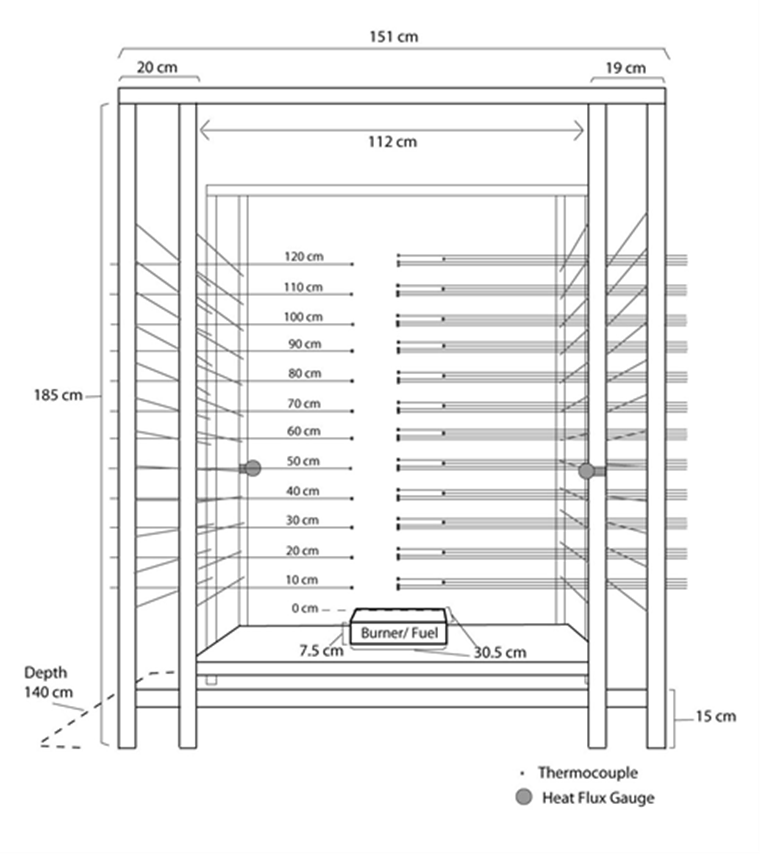
\includegraphics[width=\textwidth]{../Figures/Schematic_Drawing}\\
  \caption[Diagram of the source fire flame and plume instrumentation apparatus]{Diagram of the source fire flame and plume instrumentation apparatus which was centered under the 3~m by 3~m oxygen consumption calorimeter.  The heat flux gauges were facing toward the center of the burner/fuel area.}
  \label{Drawing_Fire_Flamer}
\end{figure}

\begin{figure}
  \centering
  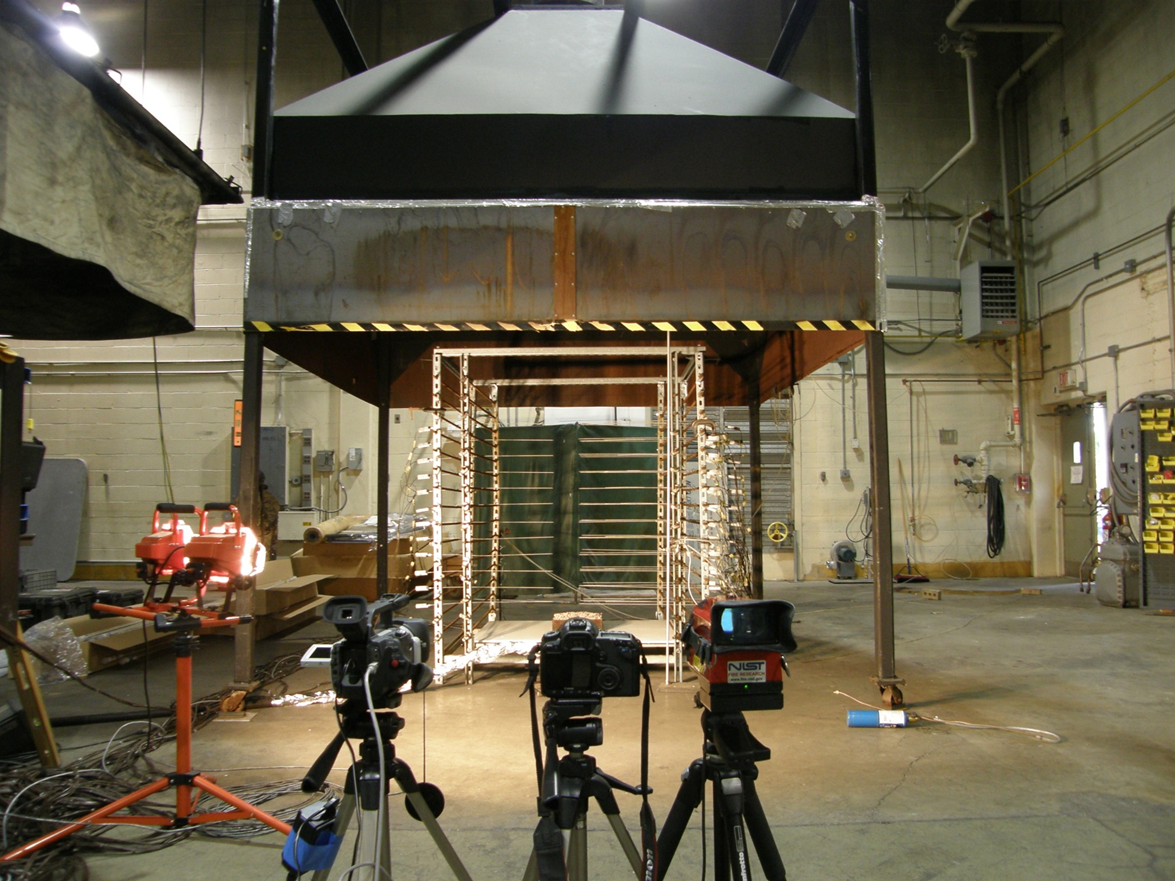
\includegraphics[width=\textwidth]{../Figures/Source_Fire_Flamer}\\
  \caption[A photograph of the source fire flamer and plume instrumentation apparatus]{A photograph of the source fire flamer and plume instrumentation apparatus which was centered under the 3~m by 3~m hood of the oxygen consumption calorimeter.  In the foreground, from left to right, are the video, 35~mm SLR and thermal imaging camera.}
  \label{Fire_Flamer}
\end{figure}



\section{Results}

\subsection{HRR}

Figures~\ref{HRR}-\ref{HRR2} show the measured heat release rates for the natural gas, gasoline and polyurethane foam fueled fires. In each graph, the replicate heat release time histories are overlaid to give a sense of the experimental repeatability for each fuel.

\begin{figure}[!ht]
  \centering
  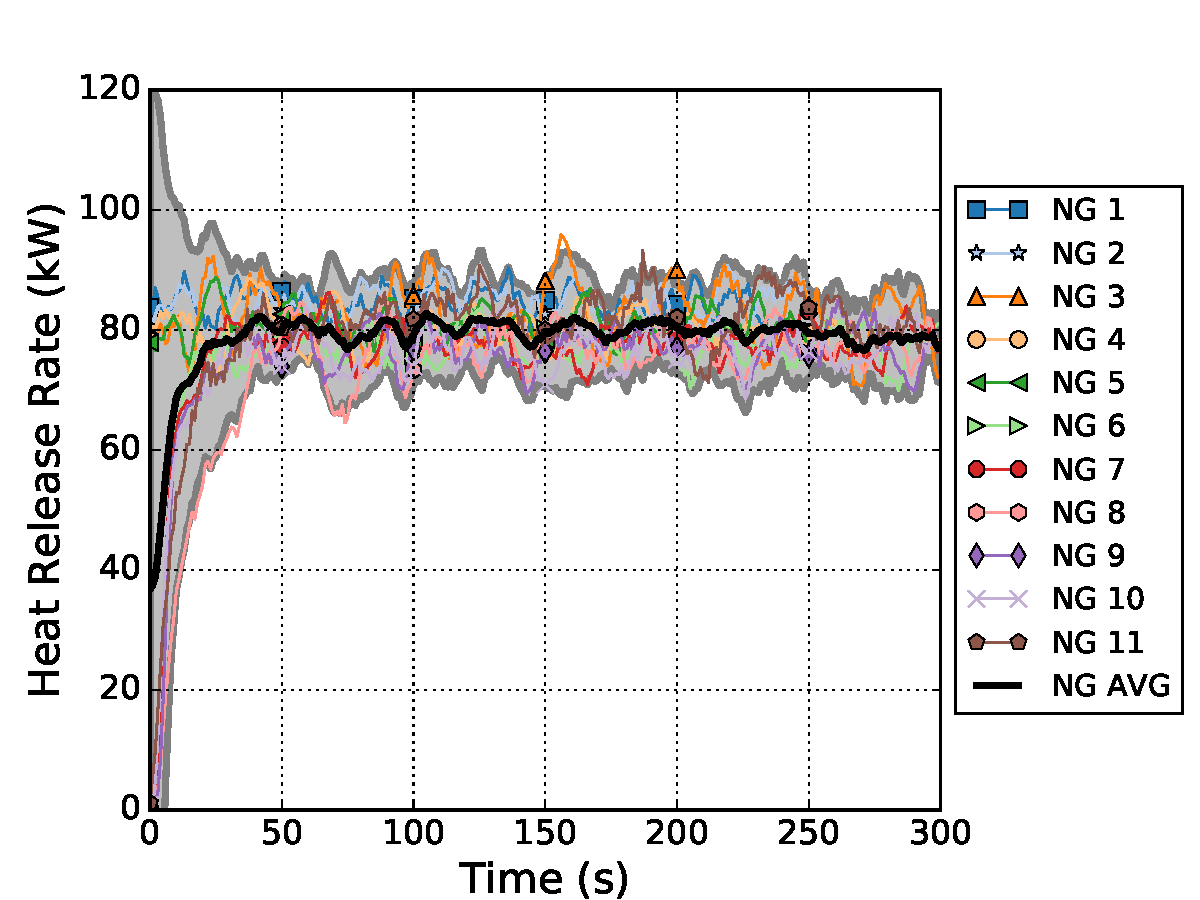
\includegraphics[width=4.5in]{../Figures/ST_NG_HRR}\\
  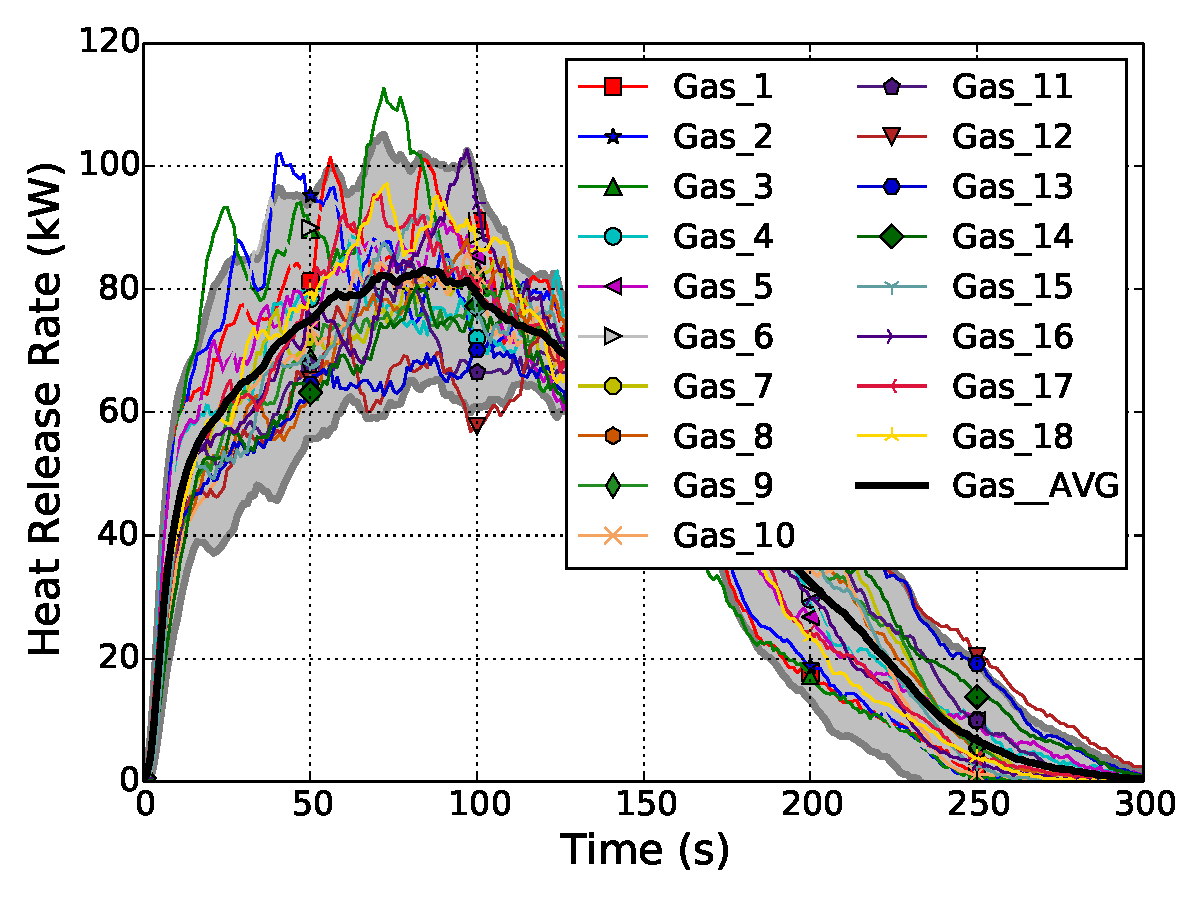
\includegraphics[width=4.5in]{../Figures/ST_Gas_HRR}\\
  \caption[Heat release rates for the natural gas and gasoline foam fires]{Heat release rates for the natural gas and gasoline fires.}
  \label{HRR}
\end{figure}

\begin{figure}[!ht]
  \centering
  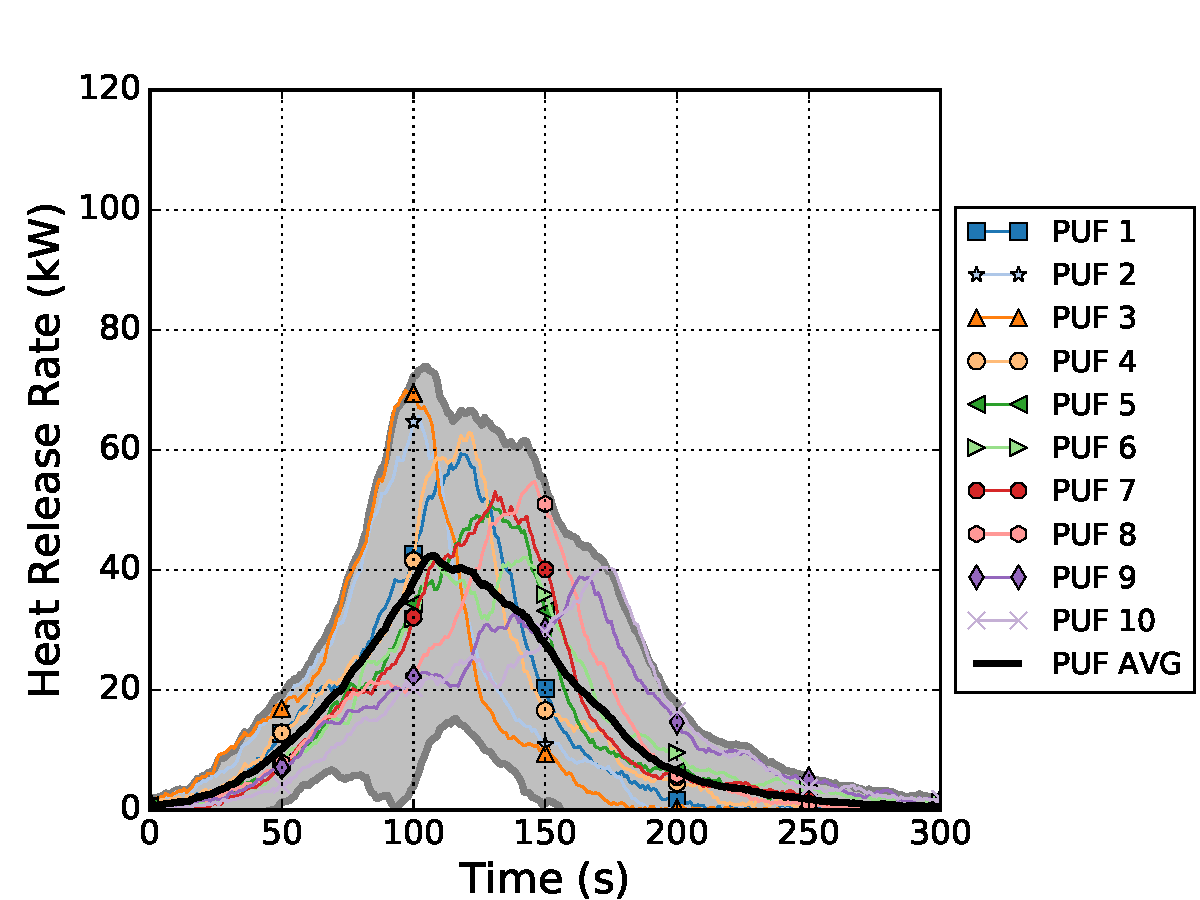
\includegraphics[width=4.5in]{../Figures/ST_PUF_HRR}\\
  \caption[Heat release rates for the polyurethane foam fires]{Heat release rates for the polyurethane foam fires.}
  \label{HRR2}
\end{figure}


On each fuel’s averaged heat release rate curve, the shaded area surrounding the average represents the 95~\% confidence level (2$\sigma$), based on Type A evaluation of the uncertainty is provided~\cite{Taylor:1994}.  A Type A evaluation of the uncertainty is any statistical analysis of the data from a series of observations.  In this case the evaluation assumed a normal distribution of the data such that doubling the calculated standard deviation (2$\sigma$) would yield a confidence level of approximately 95~\%.

The natural gas burner provided the most repeatable results, with an average steady state heat release rate of 80~kW~$\pm$~9~kW with an average total heat release of 23.3~MJ~$\pm$~1.6~MJ over a 100~s period. The uncertainty of the steady state heat release rate measurement is approximately~$\pm$~11~\% It should be noted that 11~\% is also the (2$\sigma$) uncertainty estimate of the calorimeter. The gas burner and on/off control valve allowed the heat release rate to be similar in form to a "square-wave". 

The gasoline pan fire has was ignited and then burned until the fuel was consumed.  Therefore the heat release rate curves had more of a "bell shape"  as opposed to the flat steady- state peak heat release rate region of the natural gas burner.  Therefore the  gasoline average peak heat release rate was based on an average over a 30 s interval bounding the peak heat release rate of each of the 18 experiments.  This method provided an average peak heat release rate of 80~kW~$\pm$~24~kW or 30~\%.  The total heat release of the gasoline over the 300~s period after ignition was 13.6~MJ~$\pm$~0.6~MJ.  

The block of polyurethane foam demonstrated the largest variability of the three fuels in terms of peak heat release rate and time to peak heat release. Similar to the gasoline that began with a fixed quantity of fuel which was ignitied and burned to completion, the polyurthane foam also generated "bell shaped" heat release rate curve.  Since the duration of the heat release rate peaks were less than those of the gasoline, the peak heat release rate averaging was performed over a 15~s interval bounding the peak heat release rate from each of the ten experiments.  This process yielded an average peak heat release rate of 45~kW~$\pm$~21~kW or 47~\%.  The total heat release over the 300~s period after ignition was 4.1~MJ~$\pm$~0.2~MJ. 

The Figures~\ref{HRR}-\ref{HRR2} have a shaded area that shows the 95~\% confidence level.  The more narrow the shaded area, the better the repeatability of the fire.  This provides a quick means to assess the repeatability of a given source fire.  Using this measure the natural gas burner fires were the most repeatable, followed by the gasoline pan fires and then the polyurethane fires.       


\subsection{Plume Temperatures}

Plots of the centerline temperatures averaged over the full set of replicate experiments for each of the fuels are presented in Fig.~\ref{Temp}. The natural gas temperatures are averaged over a ``steady-state'' burning period.  The temperature differences between the vertical thermocouple locations, for locations greater than 20~cm above the fire location, begin to decrease as the distances from the top of the burner increase.  This trend is similar for both the gasoline fires and the polyurethane foam fires as well.  The most notable difference between the natural gas and the other fuels is the growth and decay of the fire during the test period.

\begin{figure}[p]
  \centering
  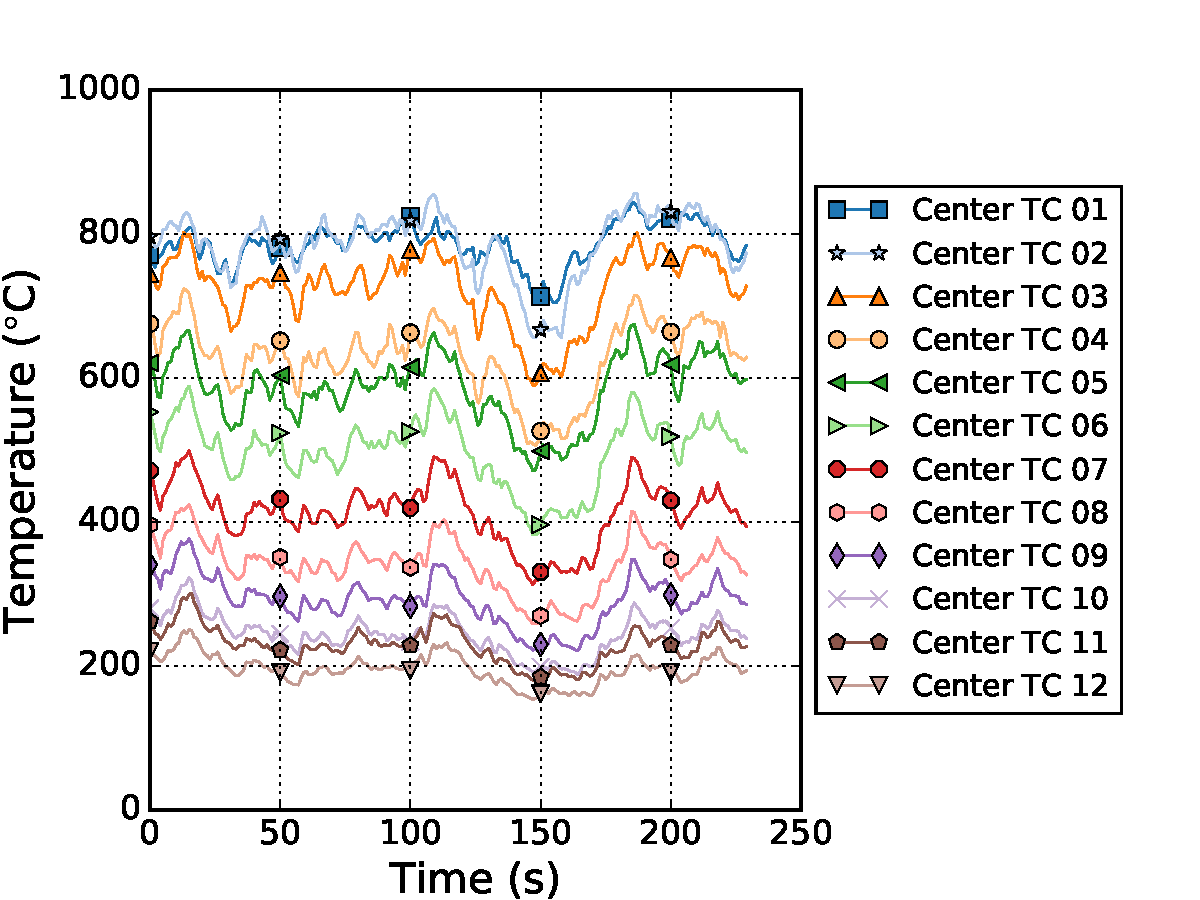
\includegraphics[width=3.5in]{../Figures/FHNG_TC_Plume_Avg}\\
  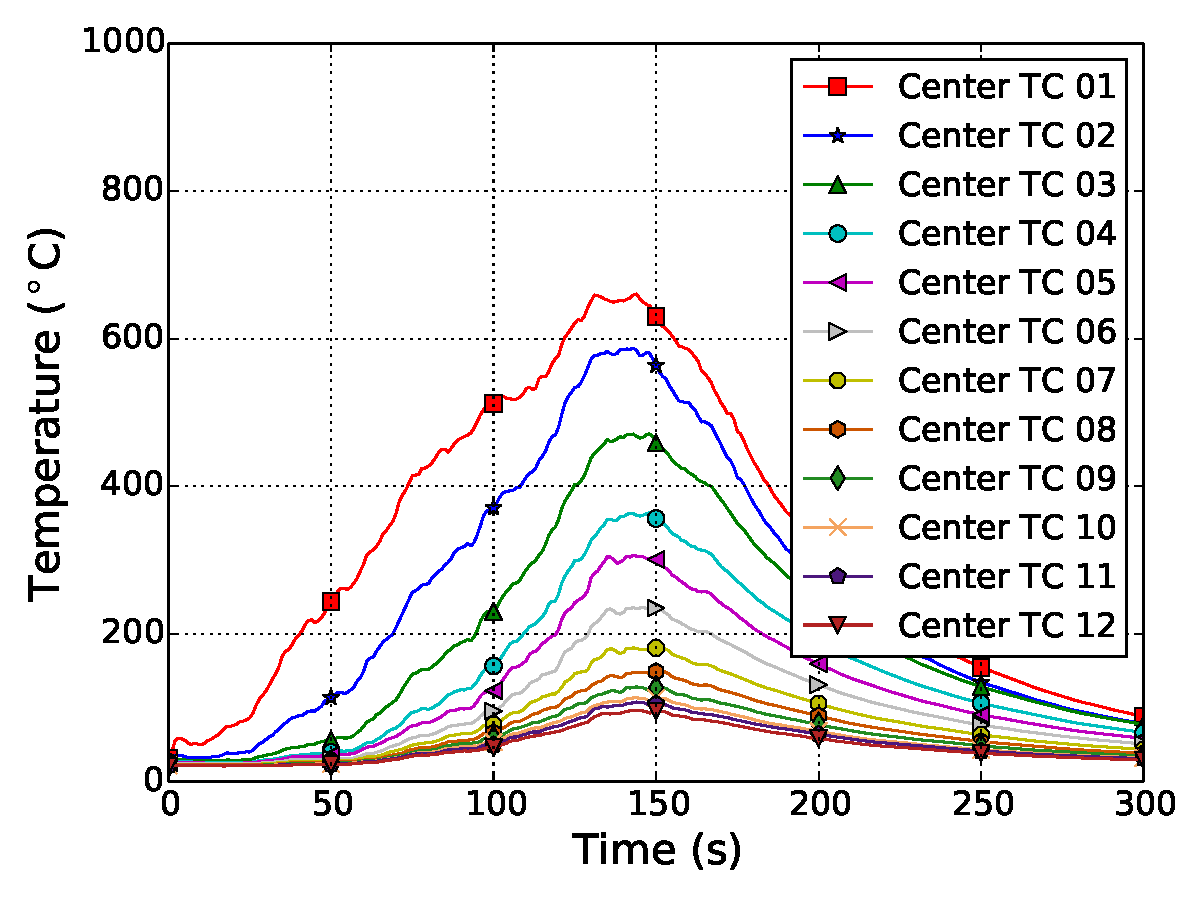
\includegraphics[width=3.5in]{../Figures/FHPUF_TC_Plume_Avg}\\
  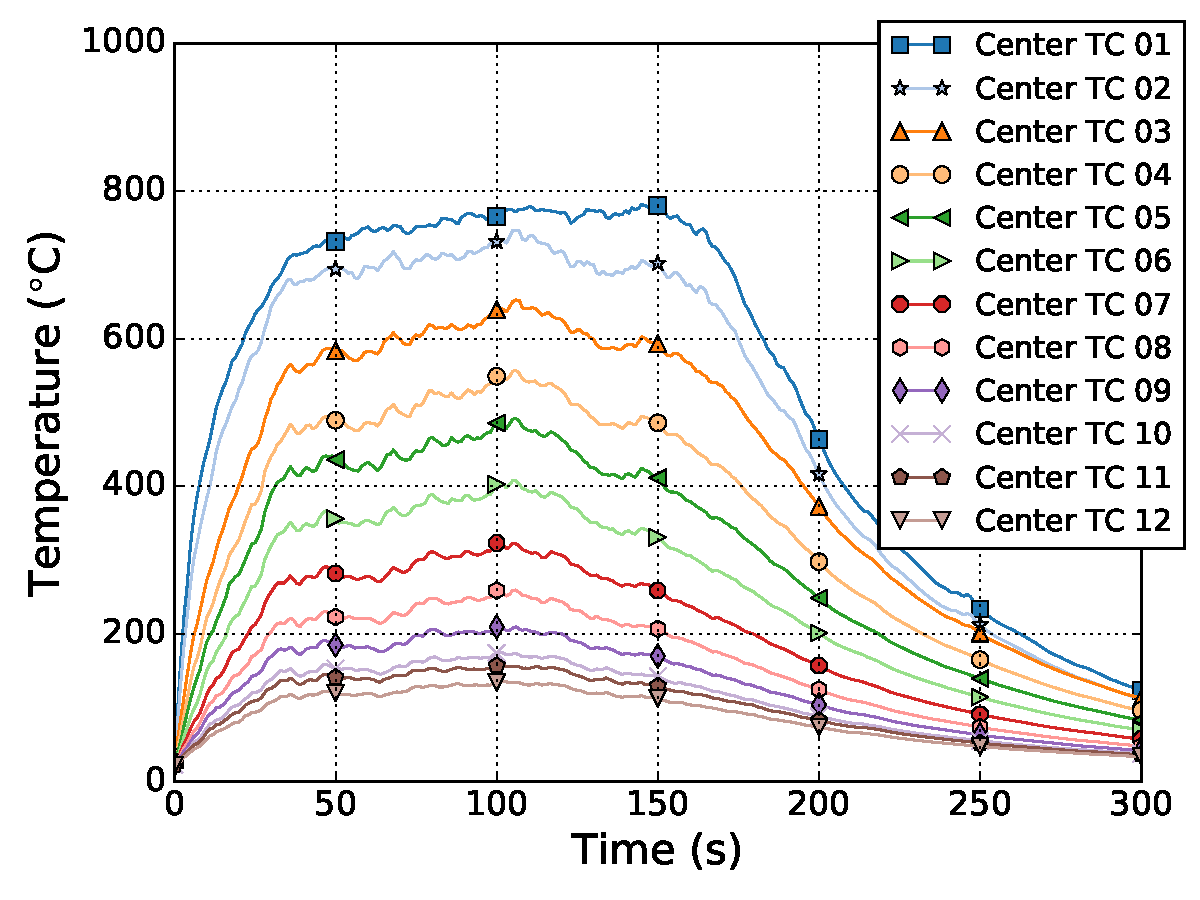
\includegraphics[width=3.5in]{../Figures/FHGAS_TC_Plume_Avg}\\
  \caption[Averaged centerline temperature for the natural gas, gasoline, and foam fires]{Averaged centerline temperature for the natural gas, gasoline, and foam fires. The number following the TC represents the height of thermocouple in decimeters above the surface of the burner.}
  \label{Temp}
\end{figure}


\subsection{Total Heat Flux}

Plots of the total heat flux for each of the fuels are presented in Fig.~\ref{Flux}. The repeatability of the total heat flux values varied in a manner similar to the heat release rates, in that the natural gas fires provided a steady state value while the gasoline and the polyurethane foam fires generated a fire curve that has periods of growth and decay.  The average peak total heat flux for the natural gas fires were approximately 2.0~kW/m$^2$.  The average peak values for the gasoline and polyurethane foam were approximately 3.5~kW/m$^2$ and 2.5~kW/m$^2$ respectively.  The values are only presented for the experiments which had two heat flux gauges installed as described in the instrumentation section above.

\begin{figure}[p]
  \centering
  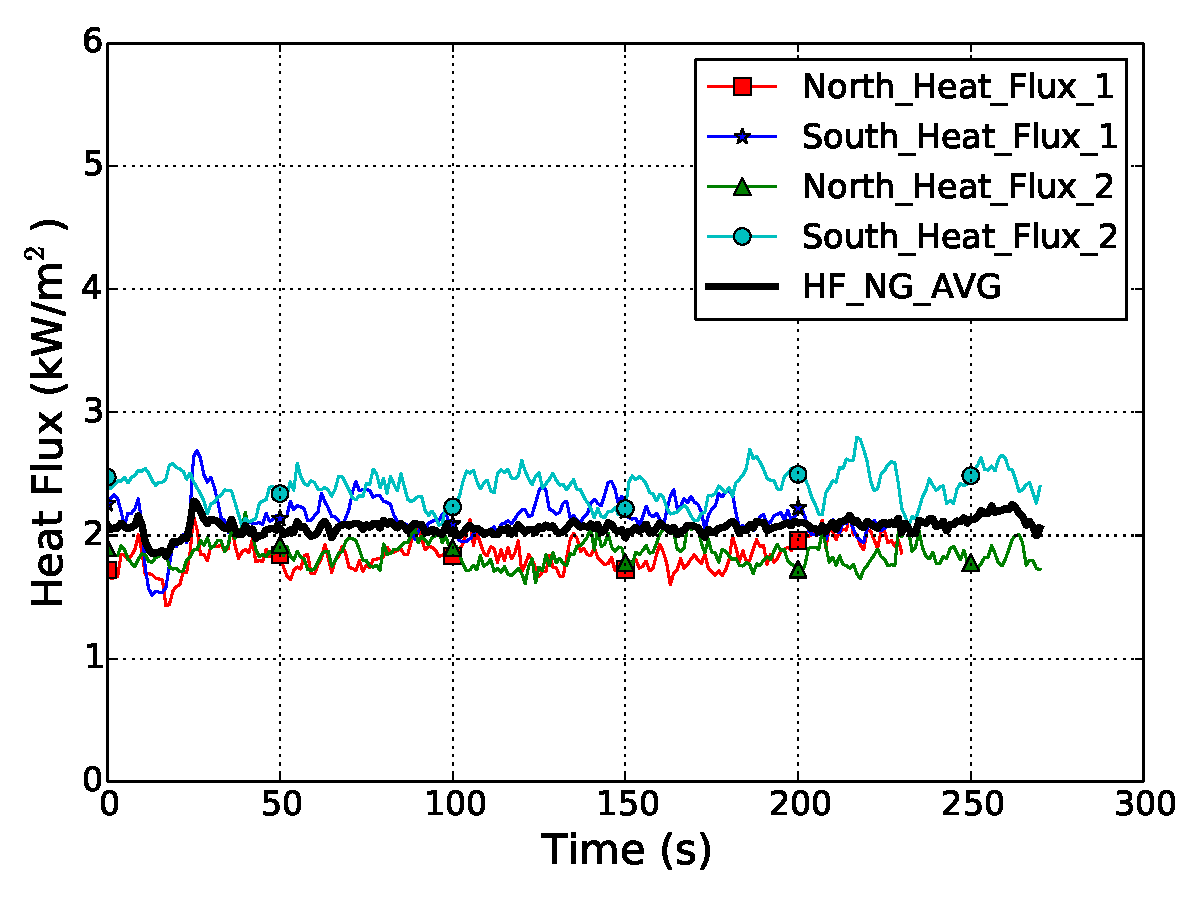
\includegraphics[width=3.5in]{../Figures/HF_NG}\\
  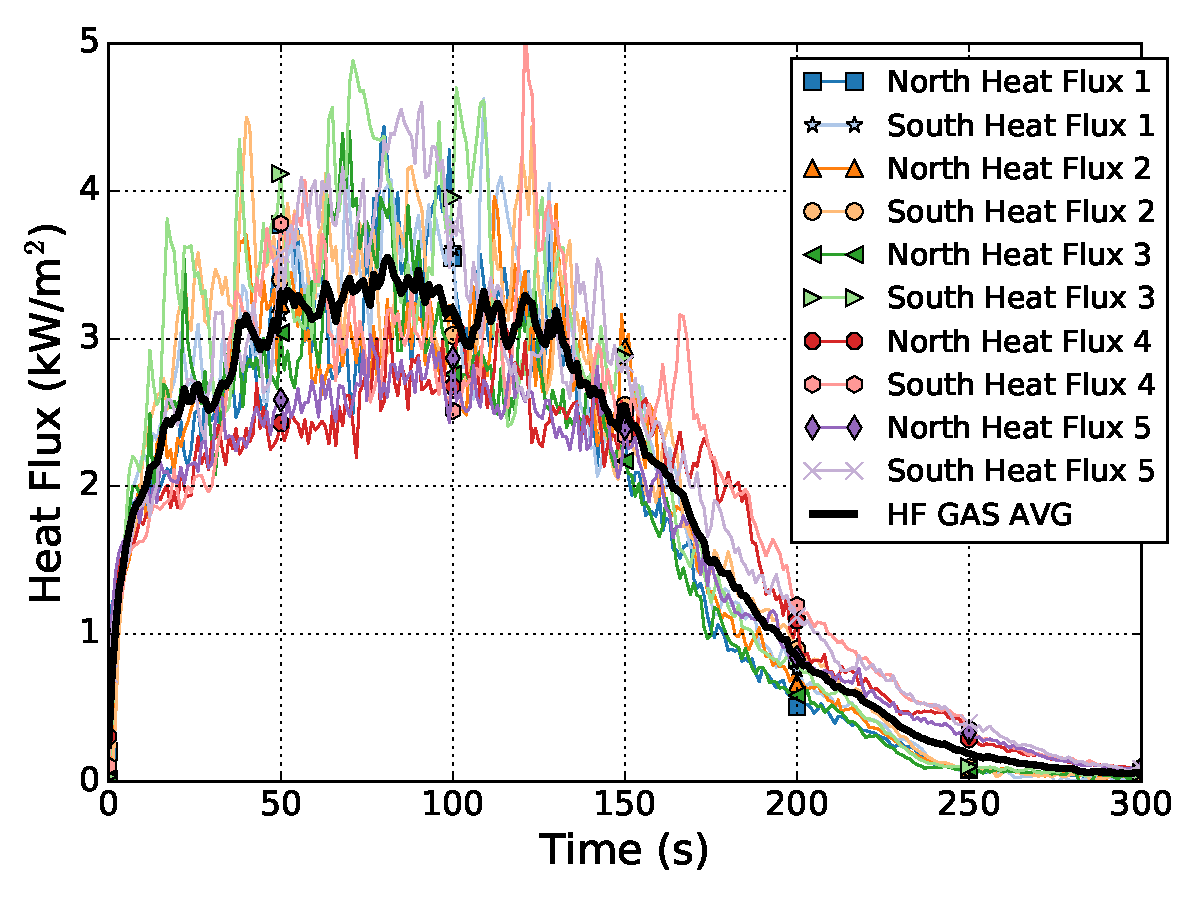
\includegraphics[width=3.5in]{../Figures/HF_GAS}\\
  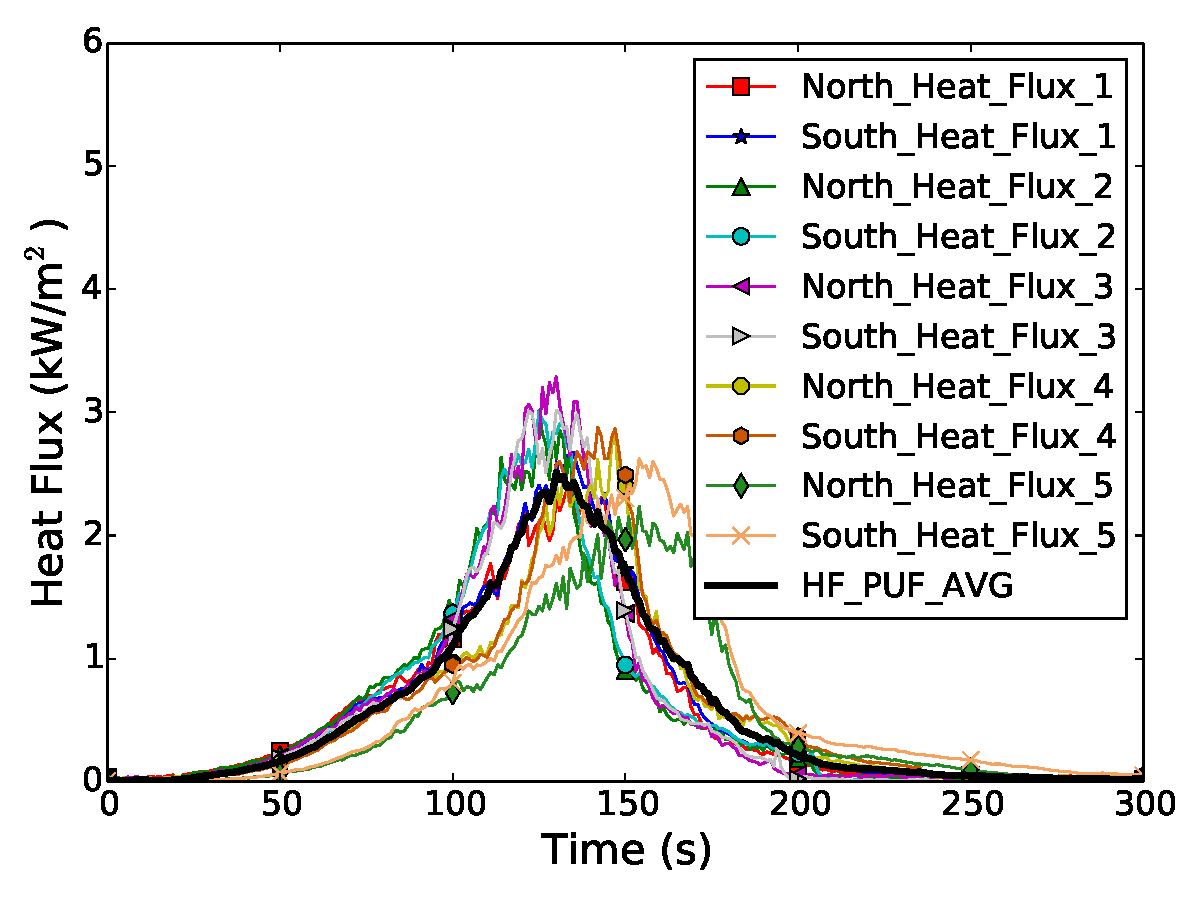
\includegraphics[width=3.5in]{../Figures/HF_PUF}\\
  \caption[Total heat flux versus time for natural gas, gasoline, and foam fires]{Total heat flux versus time for natural gas, gasoline, and foam fires.}
  \label{Flux}
\end{figure}


\subsection{Mass Loss}

Mass loss measurements were not possible for the natural gas burner experiments.  The mass loss versus time curves for the gasoline and the polyurethane experiments are shown in Fig.~\ref{Mass}.  The gasoline exhibits a linear mass loss rate for the initial 150~s of approximately 2~g/s.  The polyurethane foam was ignited with a small flame in the center of the top surface of the foam block.  As the flame spread across the surface it also began to burn down into the foam sample.  As a result the exposed surface of the foam began to take the shape of a bowl as the burning rate became linear at approximately 2~g/s.

\begin{figure}[p]
  \centering
  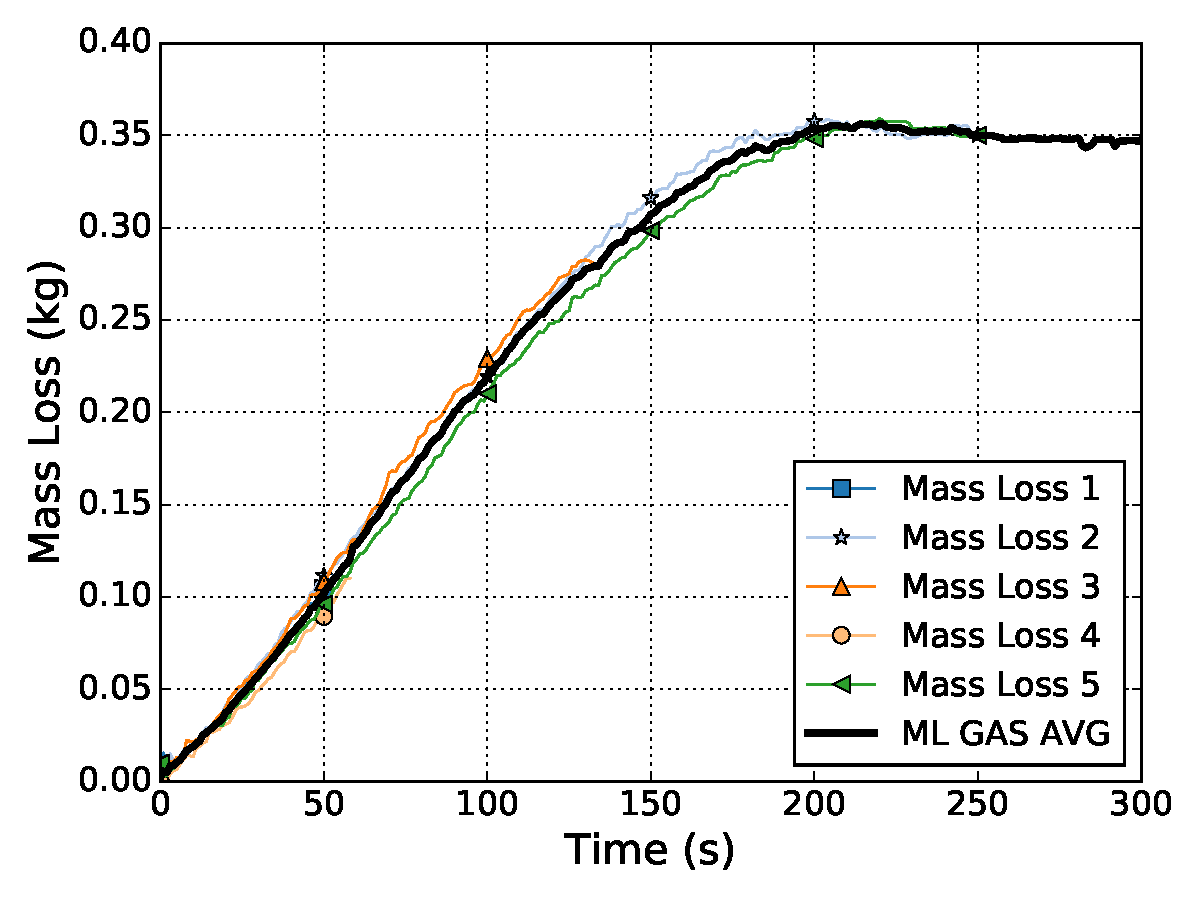
\includegraphics[width=4.5in]{../Figures/ML_GAS}\\
  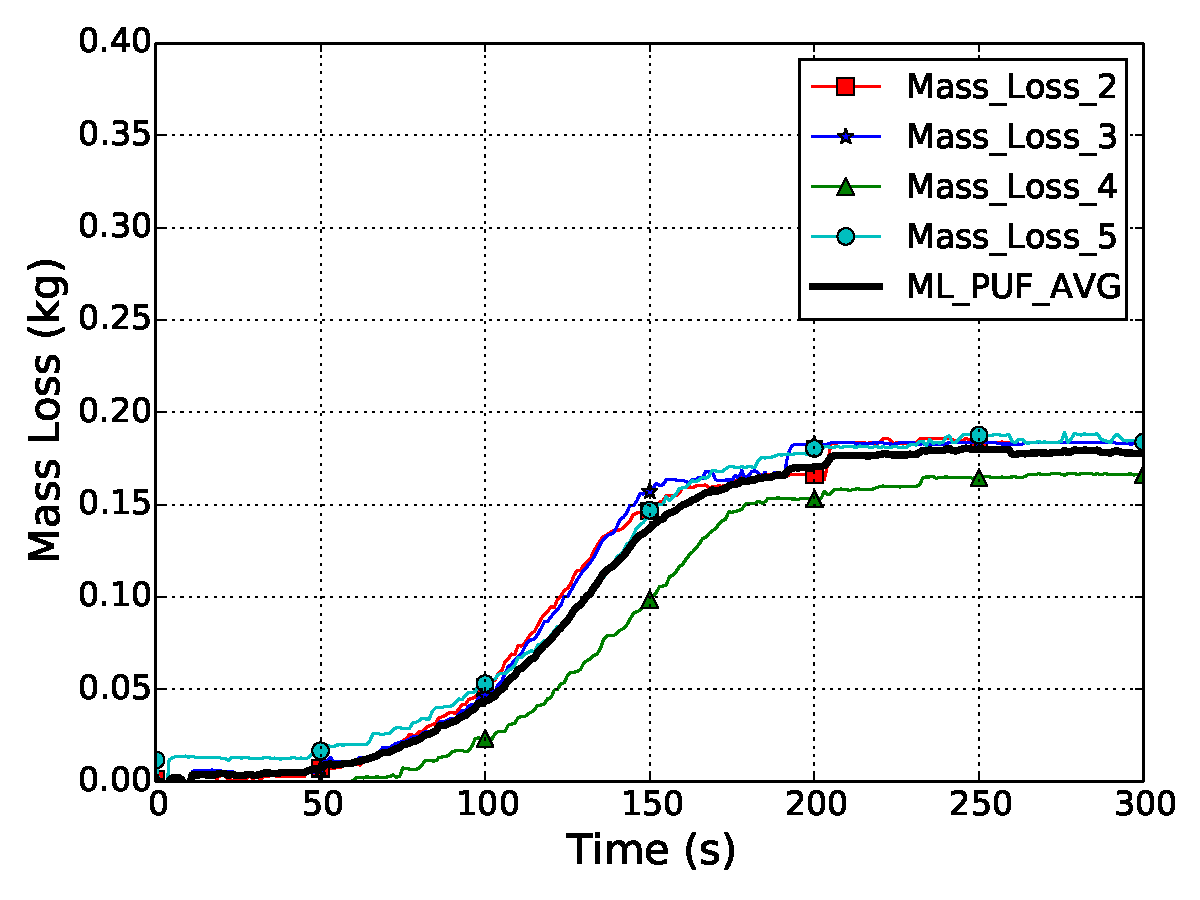
\includegraphics[width=4.5in]{../Figures/ML_PUF}\\
  \caption[Mass loss versus time for the gasoline and foam fueled fires]{Mass loss versus time for the gasoline and foam fueled fires.}
  \label{Mass}
\end{figure}


\subsection{Flame Height}

Each of the experiments was photographed with a digital single lens reflex (SLR) camera, fixed on a tripod, with a capability of capturing at least five images per second.  Located adjacent to the camera was a video camera recording images at approximately thirty 30 frames per second (fps).  The experiments were also recorded with a thermal imager, however the videos were not used for analysis as it was difficult to determine the differences between the visible flame and the thermal plume from the black and white images.

In engineering terms, the ``flame height'' is typically discussed as the median flame height.  A position above the top of the fuel surface where the flame is observed to be present at least 50~\% of the time.  As a starting point, the mean flame height for each fuel was estimated from a measurement of the uppermost continuous flame tip from the still photographic images.

Examples of the photographic images are presented in Figs.~\ref{Gas_Foam_Photos} and \ref{Gasoline_Photos}.  Figure~\ref{Gas_Foam_Photos} is a photograph of the natural gas flame taken during a period of ``steady state'' burning at approximately 80~kW and a photograph of the polyurethane foam fire taken near its peak heat release rate of approximately 60~kW.  Figure~\ref{Gasoline_Photos} presents two photographs of the same gasoline fueled fire when it was burning near its peak heat release rate of 100~kW.  The two photographs, taken 0.2~s apart, represent the range of the observed flame heights from one of the gasoline experiments from 0.65~m and 1.0~m, respectively.

\begin{figure}
  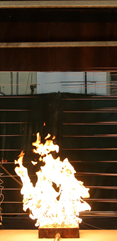
\includegraphics[height=3.5in, width=1.7in]{../Figures/NG_STFire}
  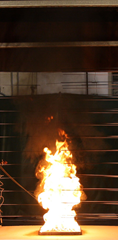
\includegraphics[height=3.5in, width=1.7in]{../Figures/Gaso_STFire} 
  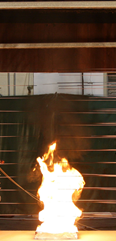
\includegraphics[height=3.5in, width=1.7in]{../Figures/PUF_STFire} \\
  \caption[Photographs of the natural gas, gasoline, and polyurethane foam fires]{Photographs showing a natural gas fire (left), gasoline fire (center), and a polyurethane foam fire (right) under the oxygen consumption calorimeter.}
  \label{Gas_Foam_Photos}
\end{figure}

\begin{figure}
  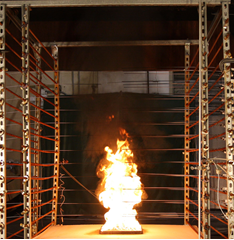
\includegraphics[width=2.6in]{../Figures/Gaso_0_65m}
  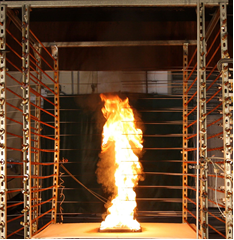
\includegraphics[width=2.6in]{../Figures/Gaso_1_0m} \\
  \caption[Photographs of the gasoline fire]{Photograph showing a gasoline fueled experiment with a flame height of 0.65~m (left) and a photograph taken approximately 0.2~s later with a flame height of 1.0~m (right).}
  \label{Gasoline_Photos}
\end{figure}


Table~\ref{tab:Flame_Heights} provides the mean visible flame height, as well as the range of flame heights for each fuel, based on analysis of the photographs for three replicate experiments.  In each case, the photographs were chosen for analysis while the fire was generating its peak heat release rate.  The range of flame heights for each fuel is approximately twice the minimum flame height or the continuous flame height. Analyzing the photographs in this manner was very time consuming and was based on making measurements on each photograph with a scale.  The limit of 5 frames per second also introduces additional uncertainty in determining the flame height. These values will serve as a basis for comparing with mean flame height values determined with video analysis.

As noted by Beyler in his review of fire plume correlations, video tape analysis seems to provide the best estimates of flame height~\cite{Beyler:1986}. Each experiment was recorded with a digital video camera at a refresh rate frequency of 29.97~fps which is the National Television Standards Committee (NTSC) standard. The resulting image in each frame was 720 pixels wide by 480 pixels high. Segments of the video which corresponded to the peak heat release of each experiment were captured with a video editing program.

For the natural gas experiments, approximately 30~s of ``steady state'' video were captured.  In the cases of the gasoline and polyurethane fueled experiments, the video capture period bounded the peak heat release rate.  In the case of the gasoline fueled fires, the peaks occurred over a long period of time, so a 30~s video capture could be made which was representative of the peak burning rate.  The peak duration for the polyurethane foam fires was shorter so, only a 15~s video capture was used.

\begin{table}
  \centering
  \begin{tabular}{|l|c|c|}
     \hline
     Fuel	            & Mean (m)  & Range (m) \\ \hline
     Natural Gas	    & 0.70	    & 0.50 to 0.98 \\
     Gasoline 	        & 0.84	    & 0.52 to 1.10 \\
     Polyurethane Foam  & 0.46	    & 0.30 to 0.78 \\
     \hline
   \end{tabular}
  \caption[Mean visible flame height and averaged minimums and maximums]{Mean visible flame height and averaged minimums and maximums (Range) of visible flame heights for each of the fuels during peak heat release rate.}
  \label{tab:Flame_Heights}
\end{table}

Each frame from the video clip was saved as a full color Tagged Image File Format (TIFF) file and the pixel aspect ratio was changed from 0.9 to 1, so that each pixel had the same dimension in both the horizontal and vertical directions.  Once these images were rendered by the video editing program, each image was scaled and cropped to provide input for Streams, a suite of image processing programs developed by Nokes for analyzing fluid flow visualization experiments~\cite{Nokes:2011}. The images were scaled so that one pixel equals 5~mm in height and width.

Examples of a set of TIFF images for each fuel are shown in Figures~\ref{flame_height_comp_FHNG80_1} through \ref{flame_height_comp_FHPUF_1}.   Each figure has 56 sequential images from the video segment.  The images total almost 2~s of actual burn time.  Notice how the flame height cycles up and down in each of the sequences.  These images provide additional information and continuity of the motion of the flame so that the analysis is less likely to miss an extreme (minimum or maximum) position when compared to the still photographs.

\begin{figure}
	\centering
	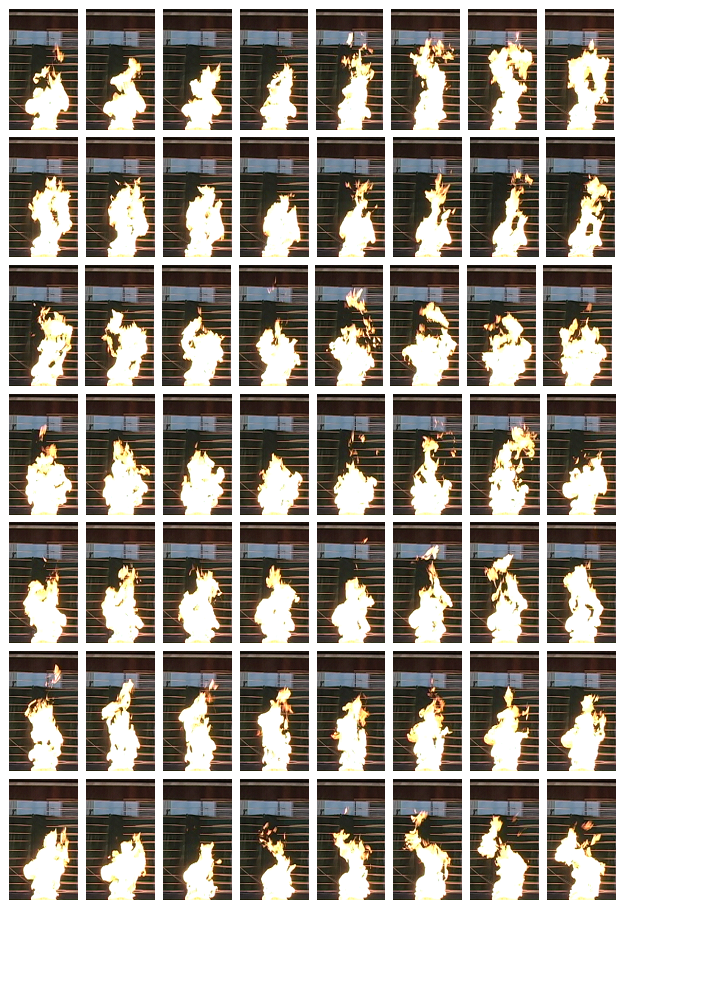
\includegraphics[width=\textwidth]{../Figures/flame_height_comp_FHNG80}\\
	\caption[Example of sequential video frames sampled from a natural gas fueled experiment]{Example of sequential video frames sampled from a natural gas fueled experiment.  In this set of images, which spans almost two seconds, the visual continuous flame height fluctuates from approximately 0.6~m to 1.1~m.}
	\label{flame_height_comp_FHNG80_1}
\end{figure}

\begin{figure}
	\centering
	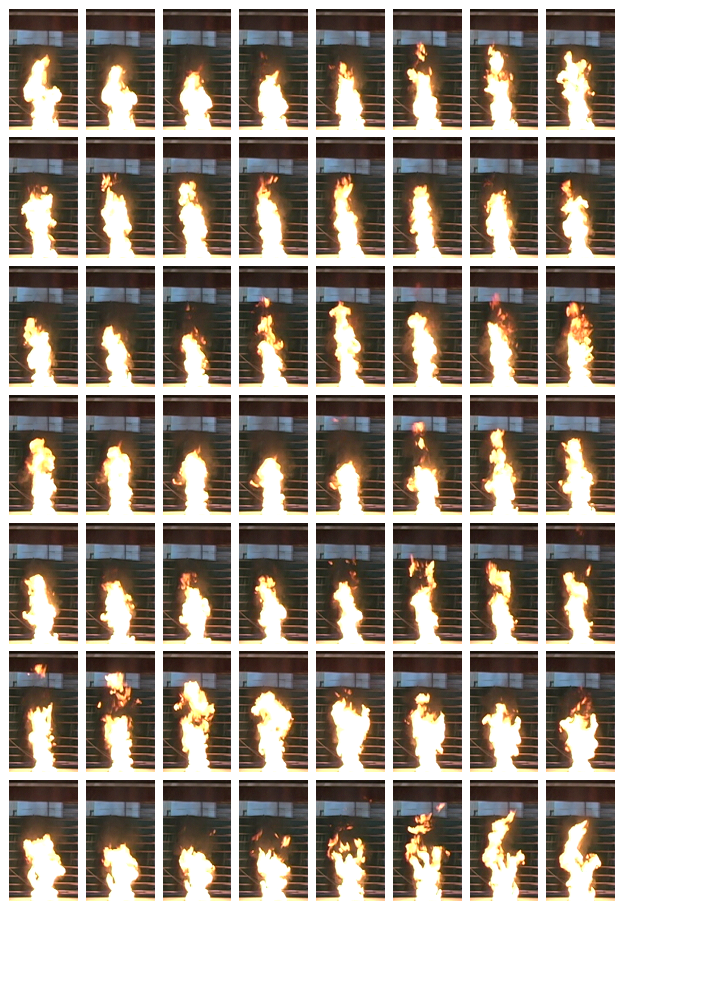
\includegraphics[width=\textwidth]{../Figures/flame_height_comp_FHGAS}\\
	\caption[Example of sequential video frames sampled from a gasoline fueled experiment]{Example of sequential video frames sampled from a gasoline fueled experiment.  In this set of images which spans almost two seconds the visual continuous flame height fluctuates from approximately 0.6~m to 1.1~m.}
	\label{flame_height_comp_FHGAS_1}
\end{figure}

\begin{figure}
	\centering
	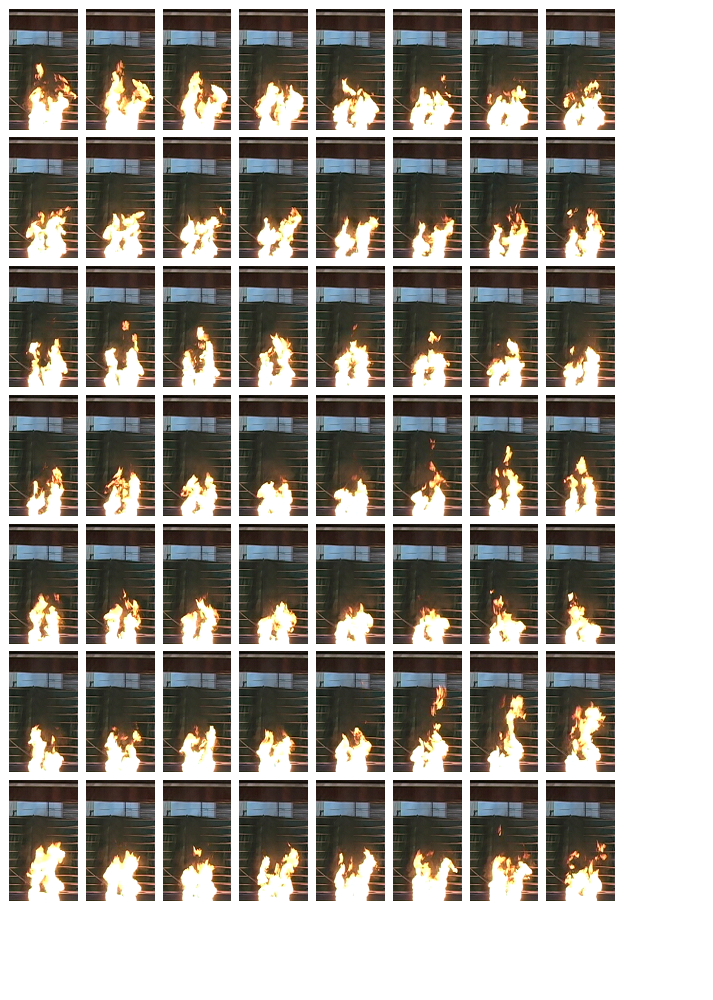
\includegraphics[width=\textwidth]{../Figures/flame_height_comp_FHPUF}\\
	\caption[Example of sequential video frames sampled from a polyurethane foam fueled experiment]{Example of sequential video frames sampled from a polyurethane foam fueled experiment.  In this set of images which spans almost two seconds the continuous visual flame height fluctuates from 0.4~m to 0.9~m.}
	\label{flame_height_comp_FHPUF_1}
\end{figure}


From each of the peak heat release rate video clips, the edited TIFF files were loaded into Streams~\cite{Nokes:2011}.  For the natural gas and gasoline fueled fires, approximately 900 images were used in each image sequence.  The polyurethane foam experiments had approximately 450 images in each sequence for each experiment.  Once the image sequence was created, a series of filters and amplifiers are applied to the images to eliminate all colors but red, based on a method developed by Goble~\cite{Goble:2007}.  Once all of the images were converted to a pure red ``flame'' which represented the area of visible fire, on a black background, the images were processed within Streams to develop an intensity field based on all of the images being ``overlaid'' on each other.  The end result is a contour plot of the intermittency of the flame ranging from zero to one.

The calculations for the intensity field are based on a user defined computation grid.  A grid sensitivity analysis was conducted with 5~mm, 10~mm, 20~mm, 40~mm and 80~mm square grids.  Examples of grid cell resolution outputs from Streams for the natural gas fueled burner are shown in Fig.~\ref{Intensity}.  The outputs shown are time averaged intensity fields generated with 5 resolutions listed above. In each output the x and y axis dimensions are in mm.

\begin{figure}[p]
	\centering
	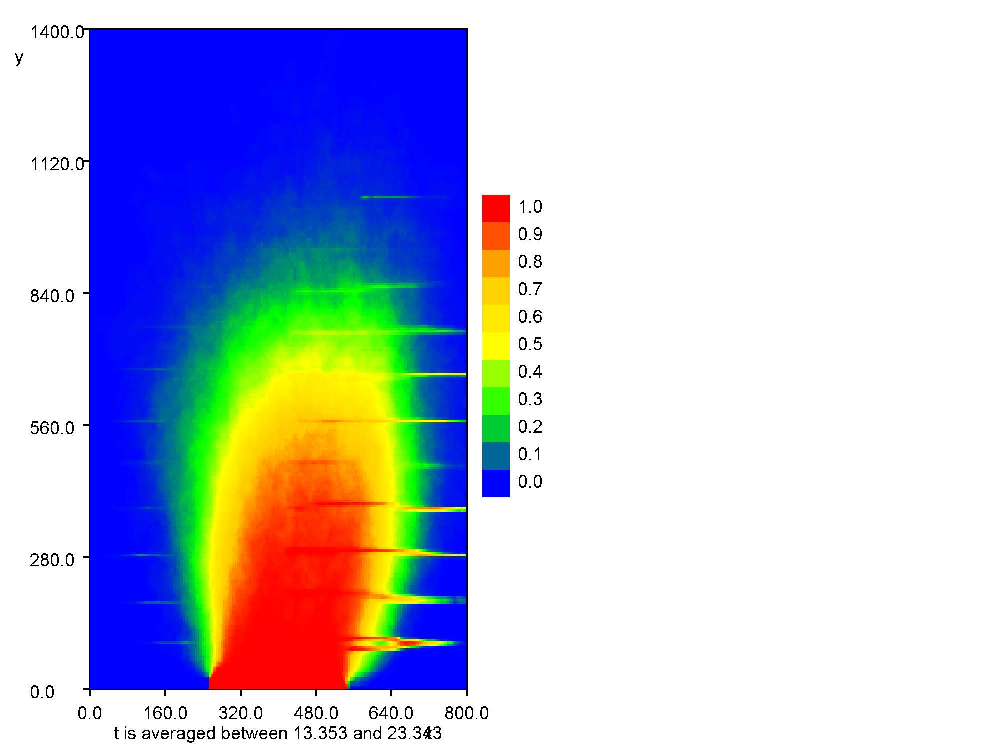
\includegraphics[trim=0in 0in 3.5in 0in,clip=true,width=1.7in]{../Figures/FHNG80_1_GS_5mm_10s_color}
	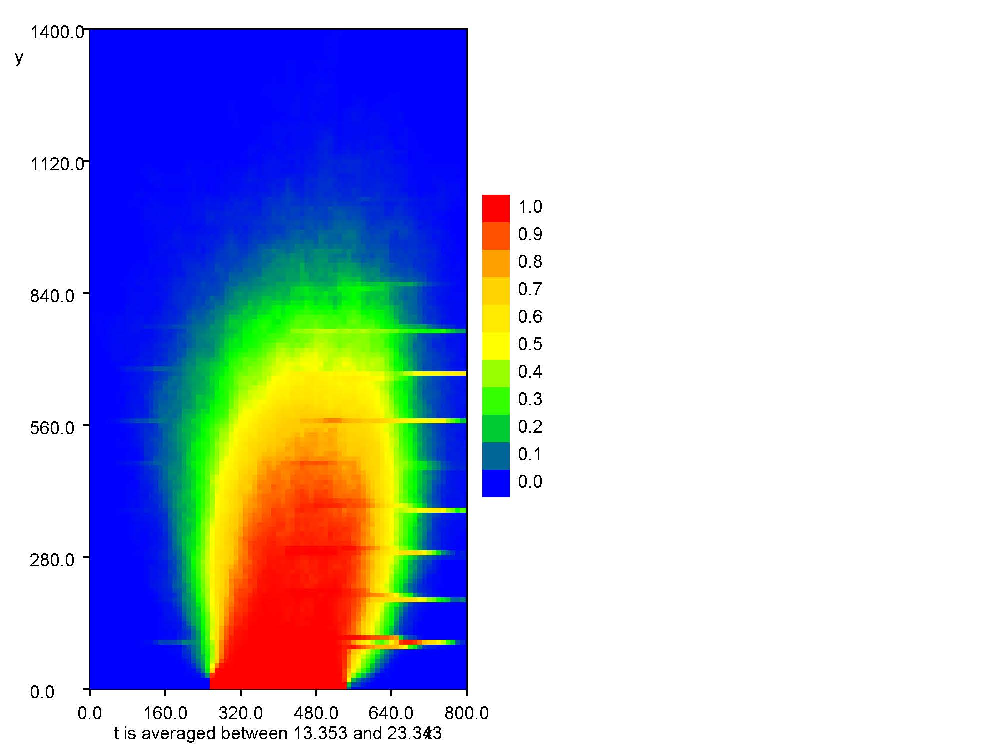
\includegraphics[trim=0in 0in 3.5in 0in,clip=true,width=1.7in]{../Figures/FHNG80_1_GS_10mm_10s_color}\\
	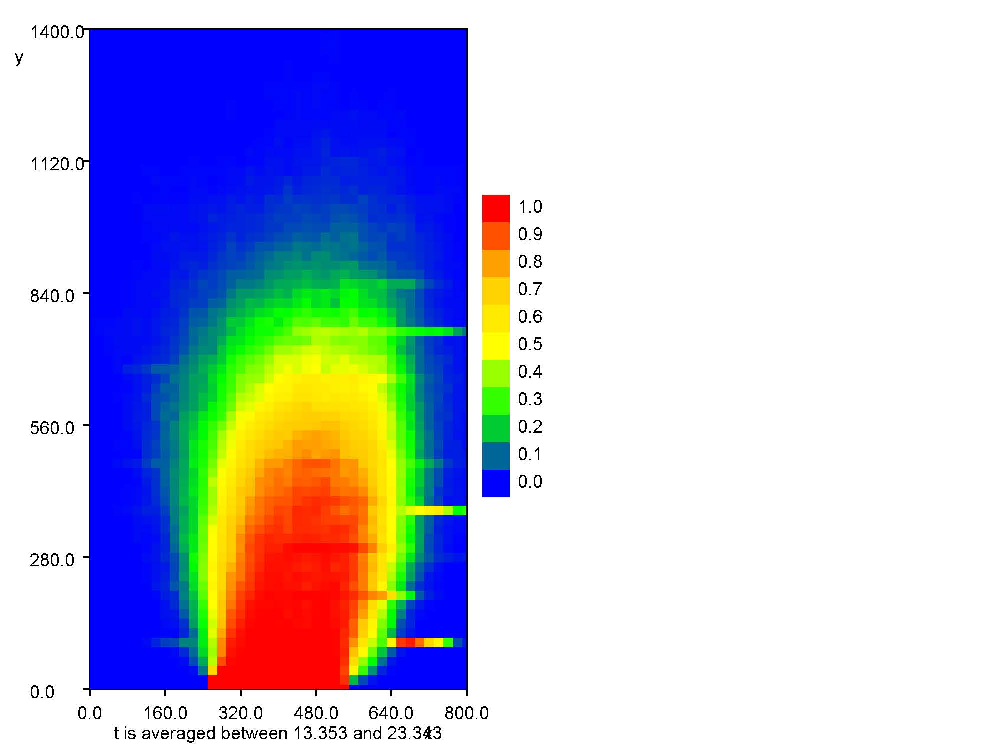
\includegraphics[trim=0in 0in 3.5in 0in,clip=true,width=1.7in]{../Figures/FHNG80_1_GS_20mm_10s_color}
	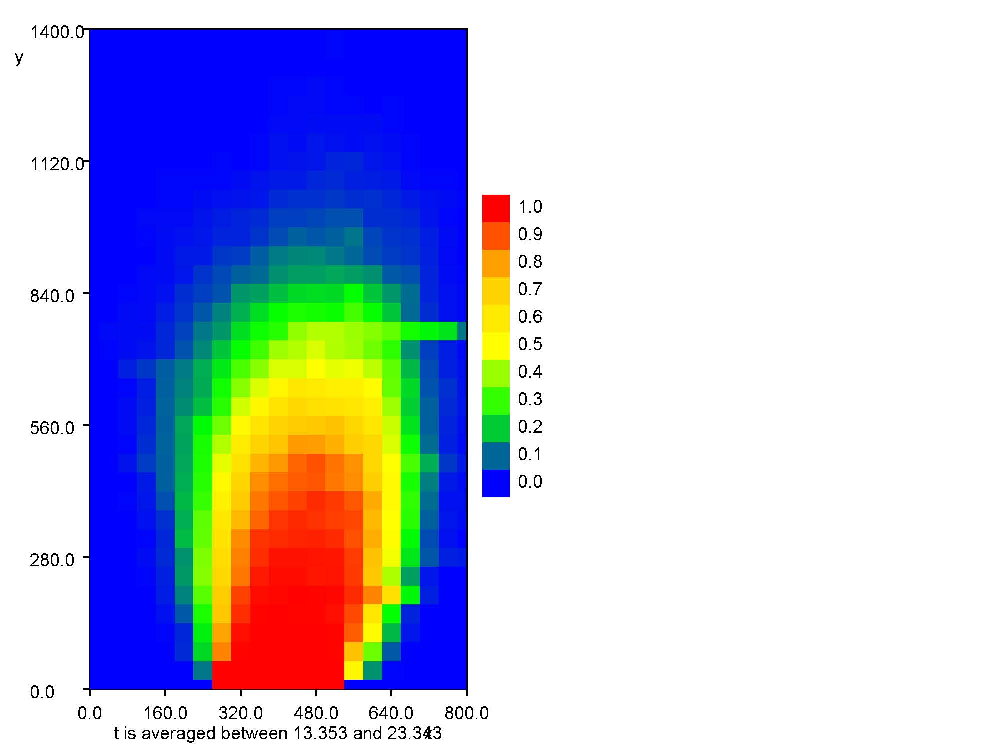
\includegraphics[trim=0in 0in 3.5in 0in,clip=true,width=1.7in]{../Figures/FHNG80_1_GS_40mm_10s_color}
	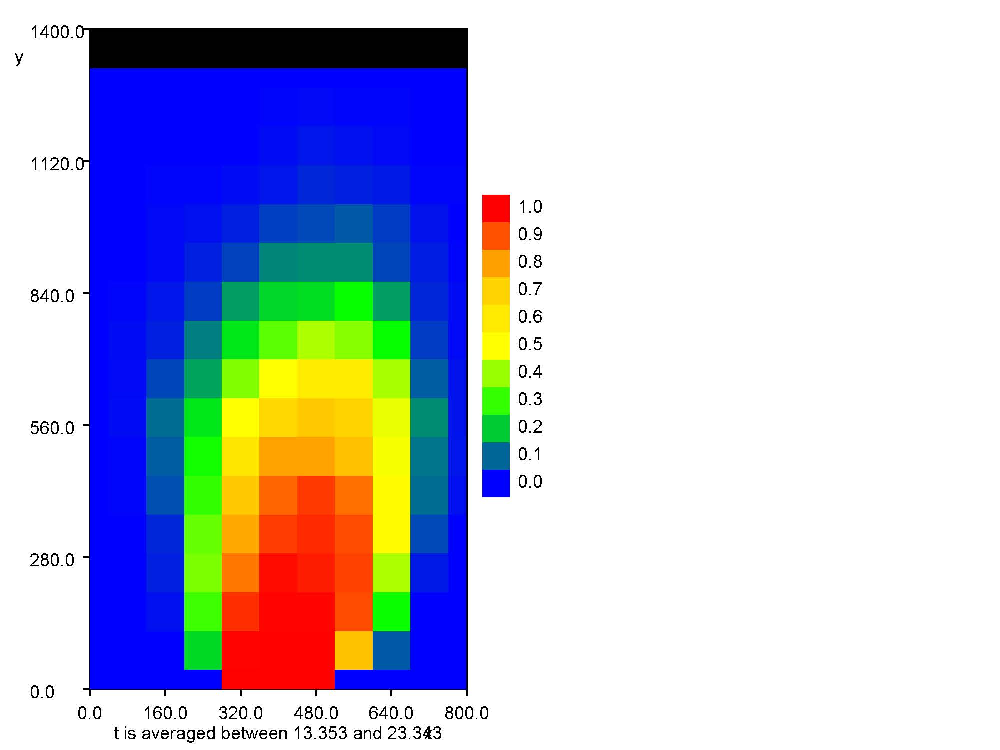
\includegraphics[trim=0in 0in 3.5in 0in,clip=true,width=1.7in]{../Figures/FHNG80_1_GS_80mm_10s_color}\\
	 \caption[Comparison images of intensity fields derived from the video images of the natural gas fueled fire]{Comparison images of intensity fields derived from the video images of the natural gas fueled fire using Streams. The images, starting with the upper left, were generated with 5~mm, 10~mm, 20~mm, 40~mm and 80~mm resolutions.}
	 \label{Intensity}
\end{figure}


Since each pixel in the original images was equal to 5~mm, in the highest resolution case, the 5~mm analysis grid would match the best resolution of the original image.  Four of the five cases resulted in similar results, only the 80~mm case generated significantly different results in flame height.  As a result of the sensitivity analysis, a 10~mm grid was chosen as an optimum size for providing a sufficient level of resolution, enabling efficient processing of 30~s worth of video frames.  At the 5~mm grid resolution, limitations within the processing system would not allow a full 30~s of video analysis.  Therefore the intensity fields and the resulting plots and data generated for this study were developed with a 10~mm grid.

Another means of quantifying field data with Streams is the use of contour plots.  Examples of the time averaged contour plots are shown in Figs.~\ref{Gas_and_Gasoline_Contours} and \ref{Foam_Contours} for the natural gas, gasoline, and polyurethane fueled fires.  Each contour line represents the percentage of time that the flame was at a given position. The region under examination, as shown as a black bounding rectangle, is 1400~mm high and 800~mm in width.  The natural gas fire was sampled for 29~s, resulting in 870~images. The area bounded by the contour with the value 1 represents the area that the flame was visible 100~\% of the time sampled. This can be considered the persistent flame region as defined by McCaffrey~\cite{McCaffrey:1979}. The remaining contours are in the intermittent flame region, with the 0.5 contour representing the mean flame height. Outside of the final contour, value 0.0, no visible flame was recorded; hence this contour marks the definitive start of the buoyant plume region.

\begin{figure}
  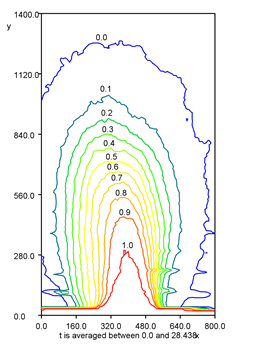
\includegraphics[width=2.7in]{../Figures/Fig20}
  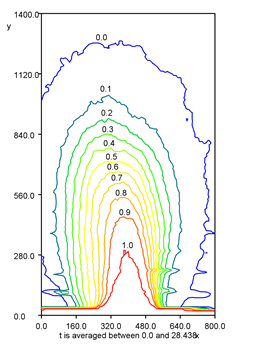
\includegraphics[width=2.7in]{../Figures/Fig21} \\
  \caption[Visibility fractions for the natural gas and gasoline fires]{Plots showing the fraction of time that the flame was visible for the natural gas (left) and gasoline (right) fires.}
  \label{Gas_and_Gasoline_Contours}
\end{figure}

\begin{figure}
  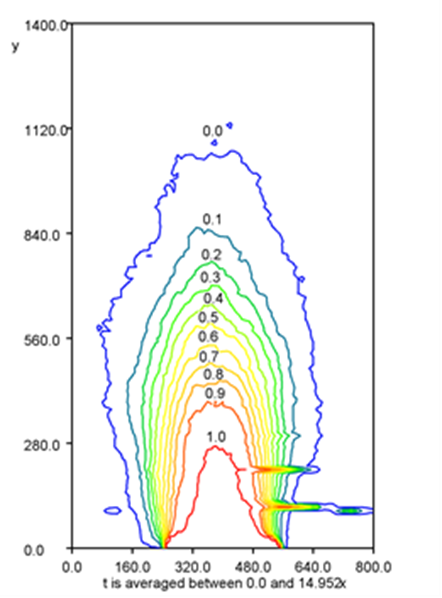
\includegraphics[width=2.7in]{../Figures/Fig22}
  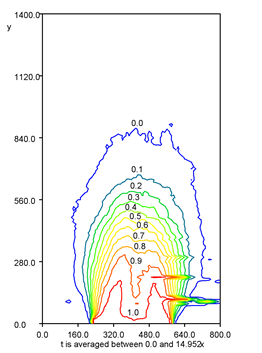
\includegraphics[width=2.7in]{../Figures/Fig23} \\
  \caption[Visibility fractions for the polyurethane foam fire]{(Left) Plot showing the fraction of time that the flame was visible for the polyurethane foam fire. (Right) Polyurethane foam contour plot with bifurcated flames at time of peak heat release rate.}
  \label{Foam_Contours}
\end{figure}

Figure~\ref{Foam_Contours} shows two different contours for the polyurethane foam fueled experiment.  The results from polyurethane fueled fire characterization experiments have an increased amount of variability due to the nature of the ignition source and the fuel itself.  The polyurethane foam was readily ignited with a small pilot flame similar to that used to ignite the natural gas and the gasoline.  By comparison, a small flame ignited the gases flowing out the top of the natural gas burner and the flames from the natural gas cover entire burner surface within approximately one second.  A similar ignition sequence occurs with the gasoline pan fires. The polyurethane foam has a more complicated flame spread sequence that resulted in significant changes to the peak heat release rate and the time to peak heat release.  Once the polyurethane foam was ignited, it took approximately 60~s for the flame to spread across the top surface of the fuel.  As the flames spread horizontally across the fuel surface, the fire also burns down into the fuel.  In some cases the fire burned completely through the fuel in the center of the foam sample, resulting in a hollow flame at the time of the peak heat release rate.  An example of a contour plot, exhibiting the hollow or bifurcated flames is shown at right in Figure~\ref{Foam_Contours}. Refer back to Figure~\ref{flame_height_comp_FHPUF_1} to see photographic views of the bifurcated flames.  It seems that the movement of the flames as they flowed away from the fuel surface blurred out the bifurcation over time with the exception of the lower elevation areas that presented at the 90 and 100~\% contours.  Other methods of ignition for the polyurethane foam were considered in order to have a more uniform ignition of the top surface of the foam.  Each method would have resulted in a larger release of energy from the ignition source or a starter fuel.   Based on a few scoping experiments these methods did not improve the repeatability.

Based on the field data developed using Streams average flame heights for each fuel were determined.  In Table~\ref{tab:Average_Flame_Heights}, each of the values represents the average flame heights, given in mm with 95~\% confidence limits based on a Type A statistical analysis of the data, for each of the source fuels shown as the percentage of time the flame was visible at that given height.  For the natural gas fires, the averages are from ten 30~s segments, while the fire was monitored at approximately 80~kW.  In some cases more than one 30~s segment was sampled per heat release rate experiment.  Sixteen 30~s video segments, which included the peak heat release rate, were successfully analyzed from the seventeen gasoline heat release rate experiments.  One of the videos was unusable for analysis due to reflected light which could not be edited out of the images.  For same reason, the polyurethane foam flame height averages are the result from eight of the ten heat release rate experiments.

\begin{table}
\centering
\begin{tabular}{|c|c|c|c|}
\hline
Visible         &   \multicolumn{3}{|c|}{Visible Flame Heights (mm)} \\ \cline{2-4}
Fraction (\%)   &       Natural Gas	            &   Gasoline	            & Polyurethane Foam \\ \hline
10              &       980 $\pm$ 155 (16~\%)   &	930 $\pm$ 130 (14~\%) 	& 650 $\pm$ 220 (34~\%)   \\
20              &   	890 $\pm$ 125 (14~\%)   &	850 $\pm$ 120 (14~\%) 	& 590 $\pm$ 190 (32~\%)   \\
30              &   	820 $\pm$ 125 (15~\%)   &	790 $\pm$ 110 (14~\%) 	& 540 $\pm$ 180 (33~\%)   \\
40              &   	760 $\pm$ 105 (14~\%)   &	740 $\pm$ 95 (13~\%) 	& 500 $\pm$ 165 (33~\%)   \\
50              &   	705 $\pm$ 106 (15~\%)   &	695 $\pm$ 95 (14~\%) 	& 470 $\pm$ 160 (34~\%)   \\
60              &   	650 $\pm$ 100 (15~\%)   &	655 $\pm$ 85 (13~\%) 	& 435 $\pm$ 135 (31~\%)   \\
70              &   	590 $\pm$ 90 (15~\%)    &	610 $\pm$ 90 (15~\%) 	& 400 $\pm$ 125 (31~\%)   \\
80              &   	530 $\pm$ 85 (16~\%)    &	555 $\pm$ 90 (16~\%) 	& 360 $\pm$ 110 (31~\%)   \\
90              &   	440 $\pm$ 75 (17~\%)    &	490 $\pm$ 95 (19~\%) 	& 315 $\pm$ 110 (35~\%)   \\
100	            &       220 $\pm$ 84 (38~\%)    &	350 $\pm$ 110 (32~\%) 	& 210 $\pm$ 125 (60~\%)   \\
\hline
\end{tabular}
 \caption[Average flame heights for three fuels]{Average flame heights with 95~\% confidence limits, for each of the source fuels shown as the percentage of time the flame was visible at that given height.}
 \label{tab:Average_Flame_Heights}
\end{table}


For both the natural gas and the gasoline experiments the 95~\% confidence limits show less than 20 percent variation in visible flame height within the intermittent flame region.  The percentage variation increases at the continuous flame region, although the magnitudes of the height variations are similar to other sections of the intermittent flame region.  The percentage variation is higher in the continuous flame region because the height of the continuous flame region is the smallest.  The 95~\% confidence limits for the polyurethane foam are about twice those of the natural gas and the gasoline.

\subsection{Summary}

The source fires have been characterized in terms of heat release rate, plume temperature, total heat flux, mass loss and flame height.  This data has been collected for use in direct analysis of the burn patterns and as input into the engineering correlations and FDS models that are used later in this study.



\chapter{Instrumented Non-combustible Wall Experiments}

Once the characteristics of the fires had been measured, the next step was to measure the thermal impact that the fires had on a vertical target surface.  In these experiments the target is a non-combustible wall. The non-combustible material was chosen to prevent any contribution due to combustion from the wall to the fire.  The fires were placed at predetermined, fixed positions away from the wall. The fires were prepared and conducted in the same manner as the they were in the fire characterization experiments. As a result the exposure time of the target wall to the fire was 300 seconds. In the remainder of the report the term burner will be considered synonymous with the pan for the liquid fuel or the block of solid fuel. Experiments were conducted with the closest edge of the burner located in the following positions from the wall: two burner widths (0.610~m), one burner width (0.305~m), one half burner width (0.150~m), and then touching the wall (0.0~m).


\section{Experimental Arrangement}

A free standing steel frame wall with a 12.7~mm thick, 2.44~m high by 1.22~m wide, calcium silicate board face was instrumented to measure the thermal exposure of the wall from the fire in terms of temperature and heat flux. Marinite Type I is the commercial name of the non-combustible board used in these experiments.  It is normally used as a fire-resistant thermal insulation that also has structural strength. 90~\% of the board is composed of calcium silicate and calcium meta-silicate.  The remaining 10~\% of the board is composed of a combination of organic fibers, fiber glass filament and crystalline silica (quartz)~\cite{BNZ:MSDS}.  Material properties that impact heat transfer were selected from the manufacturer's literature and are presented In Table~\ref{tab:Marinite_Thermal_Properties}~\cite{Marinite:1997}.

\begin{table}
	\centering
\begin{tabular}{|c|c|c|c|c|}
	\hline Density & \multicolumn{2}{c|}{Thermal Conductivity} & \multicolumn{2}{c|}{Specific Heat}   \\
    \hline (kg/m$^3$) & Temperature ($^\circ$C) & (W/mK)  & Temperature ($^\circ$C)  & (kJ/kg $^\circ$C) \\
	\hline 737  & 24 & 0.13 & 93 & 0.28 \\
	\hline  & 205 & 0.12  & 205 & 0.30 \\
	\hline  & 316 & 0.11 & 316 & 0.32 \\
	\hline  & 425 & 0.12 & 425 & 0.34 \\
	\hline  & 538 & 0.12 &  &  \\
	\hline
\end{tabular}
\caption[Thermal properties for Marinite I]{Thermal properties for Marinite I, as reported by the manufacturer BNZ~\cite{Marinite:1997}}
\label{tab:Marinite_Thermal_Properties}
\end{table}

Two vertical arrays of water cooled, Schmidt-Boelter total heat flux gauges, as previously described in the instrumentation section above, were installed at 20 cm intervals from 0.2~m to 1.2~m above the burner.  One vertical array was centered on the burner and the other vertical array was centered on the right edge of the burner. The arrangement is shown in Fig.~\ref{Instrumented_NC_Wall}. Bare-bead, Chromel-Alumel (type K) thermocouples, with a 0.5~mm nominal diameter were installed next to the center of each heat flux sensors and continued, at 20~cm intervals, up to a height of 2.2~m above the surface of the burner. Photographs of the front and rear of the instrumented wall are shown in Figures~\ref{Instrumented_Wall_Front_photo} and \ref{Instrumented_Wall_Rear_photo} The thermocouples where installed in small holes from the back of the wall.  The bead of the thermocouple was flush with the surface on the calcium silcate board and was in contact with the board, as shown in Figure~\ref{Instrumented_Wall_Close_up_TC_HF_photo} For the center array,a second thermocouple was installed on the backside of the calcium silicate board, approximately 10~mm below the TC positioned on the front surface of the wall. The photograph in Figure~\ref{Instrumented_Wall_Detail_Rear_TC_photo} shows a rear thermocouple with the bead in contact with the rear surface of the wall and the relative position to the thermocouple on the front surface of the wall. In a manner similar to the source fire characterization experiments, the instrumented wall experiments were conducted under the NIST Large Fire Research Laboratory's 3~m by 3~m oxygen depletion calorimeter.

\begin{figure}
	\centering
	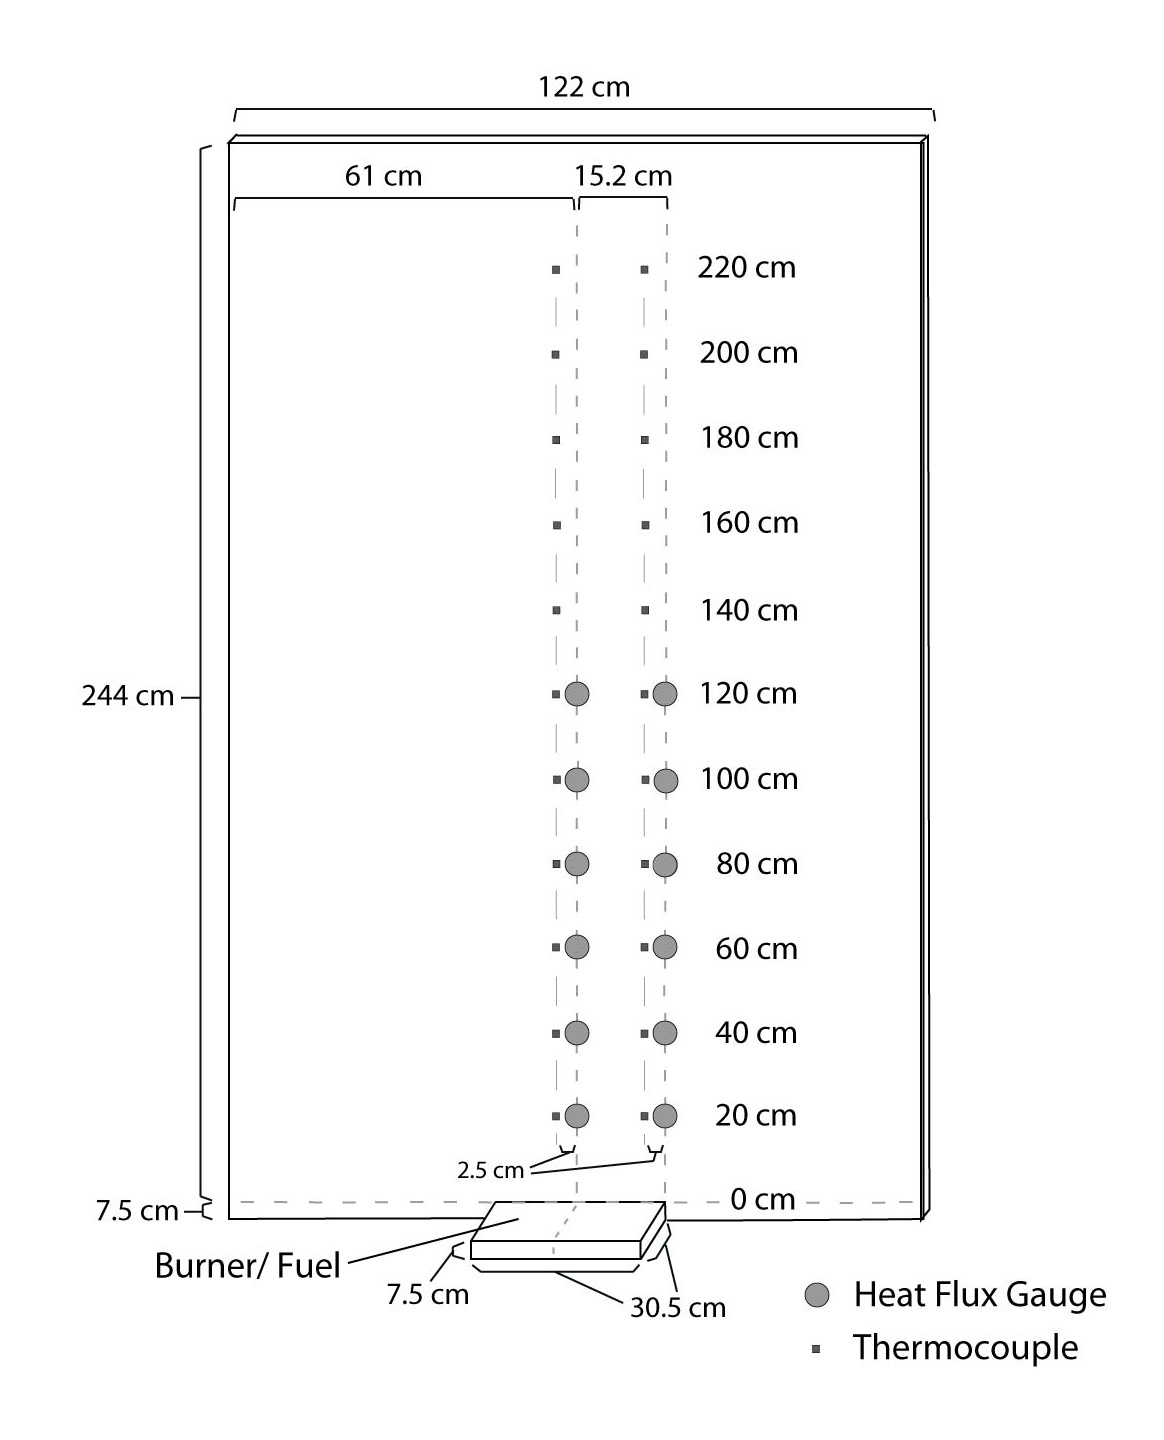
\includegraphics[width=\textwidth]{../Figures/Instrumented_NC_Wall}\\
	\caption[Diagram of the instrumented non-combustible wall]{Diagram of the instrumented non-combustible wall. Two vertical arrays of total heat flux gauges and thermocouples were installed along the centerline of the burner and along the right edge of the burner.}
	\label{Instrumented_NC_Wall}
\end{figure}

\begin{figure}
	\centering
	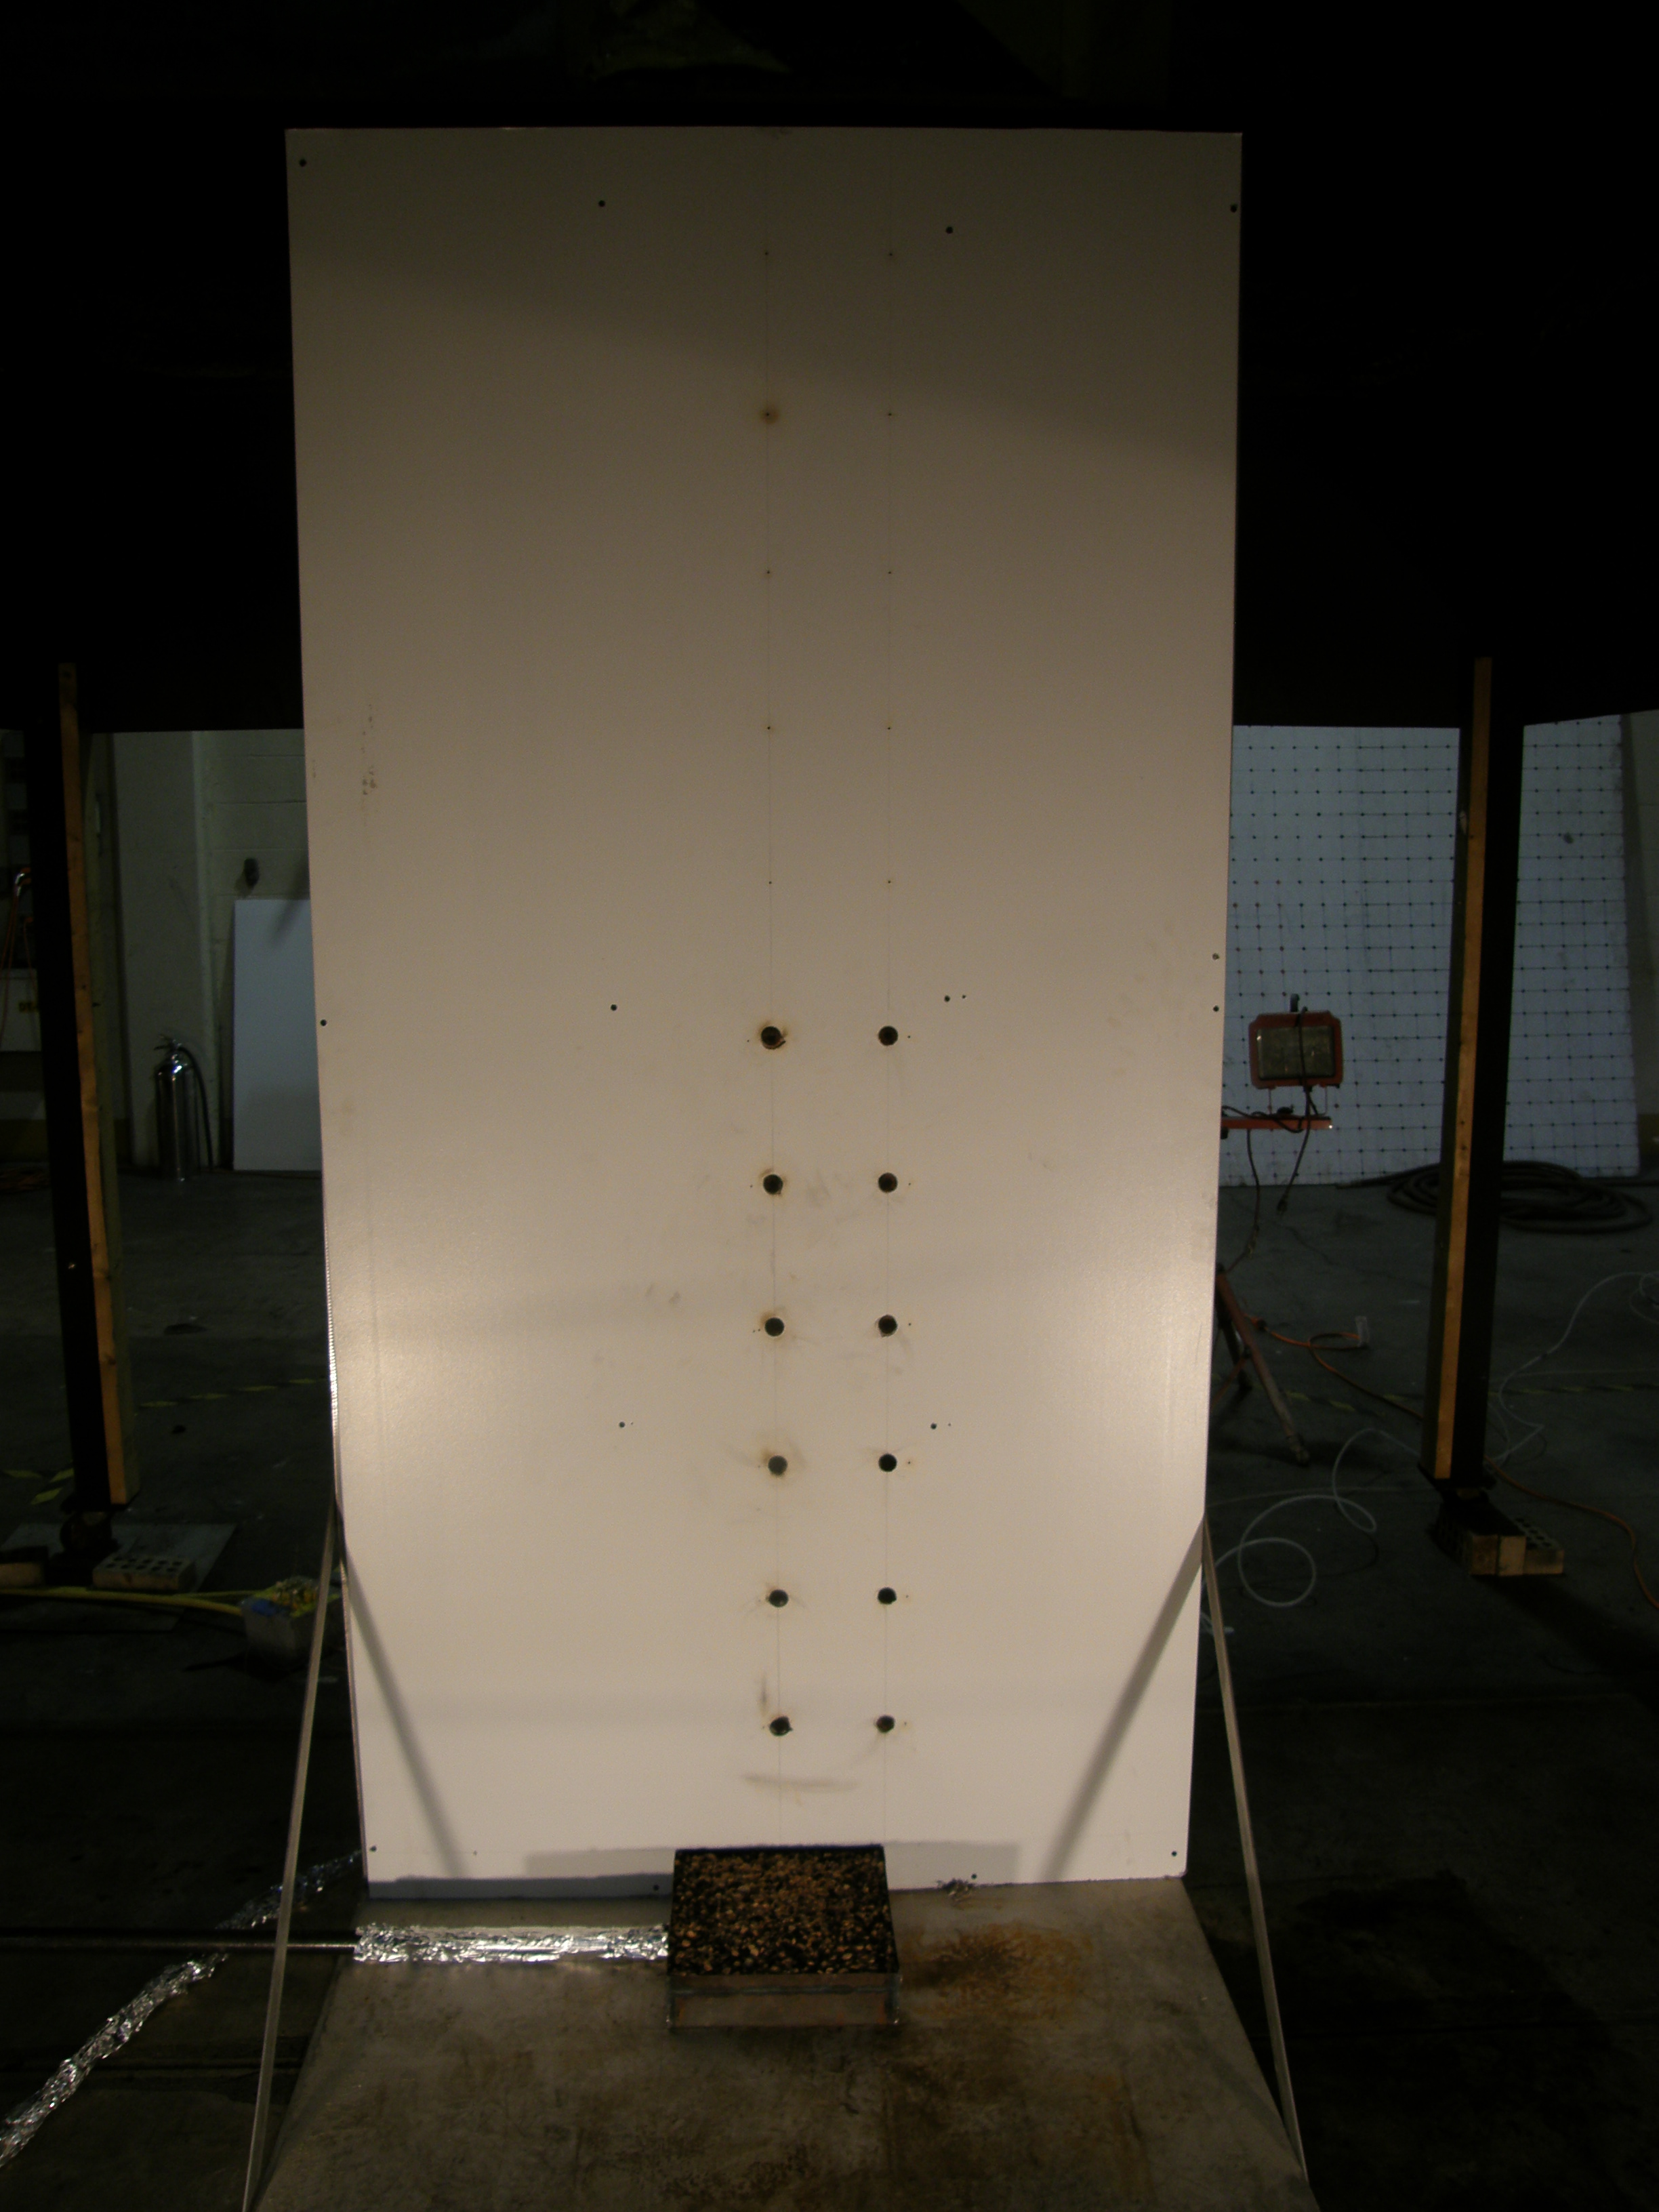
\includegraphics[width=\textwidth]{../Figures/Instrumented_Wall_Front_photo}\\
	\caption[Photograph of the front side of the instrumented non-combustible wall]{Photograph of the front side of the instrumented non-combustible wall.}
	\label{Instrumented_Wall_Front_photo}
\end{figure}

\begin{figure}
	\centering
	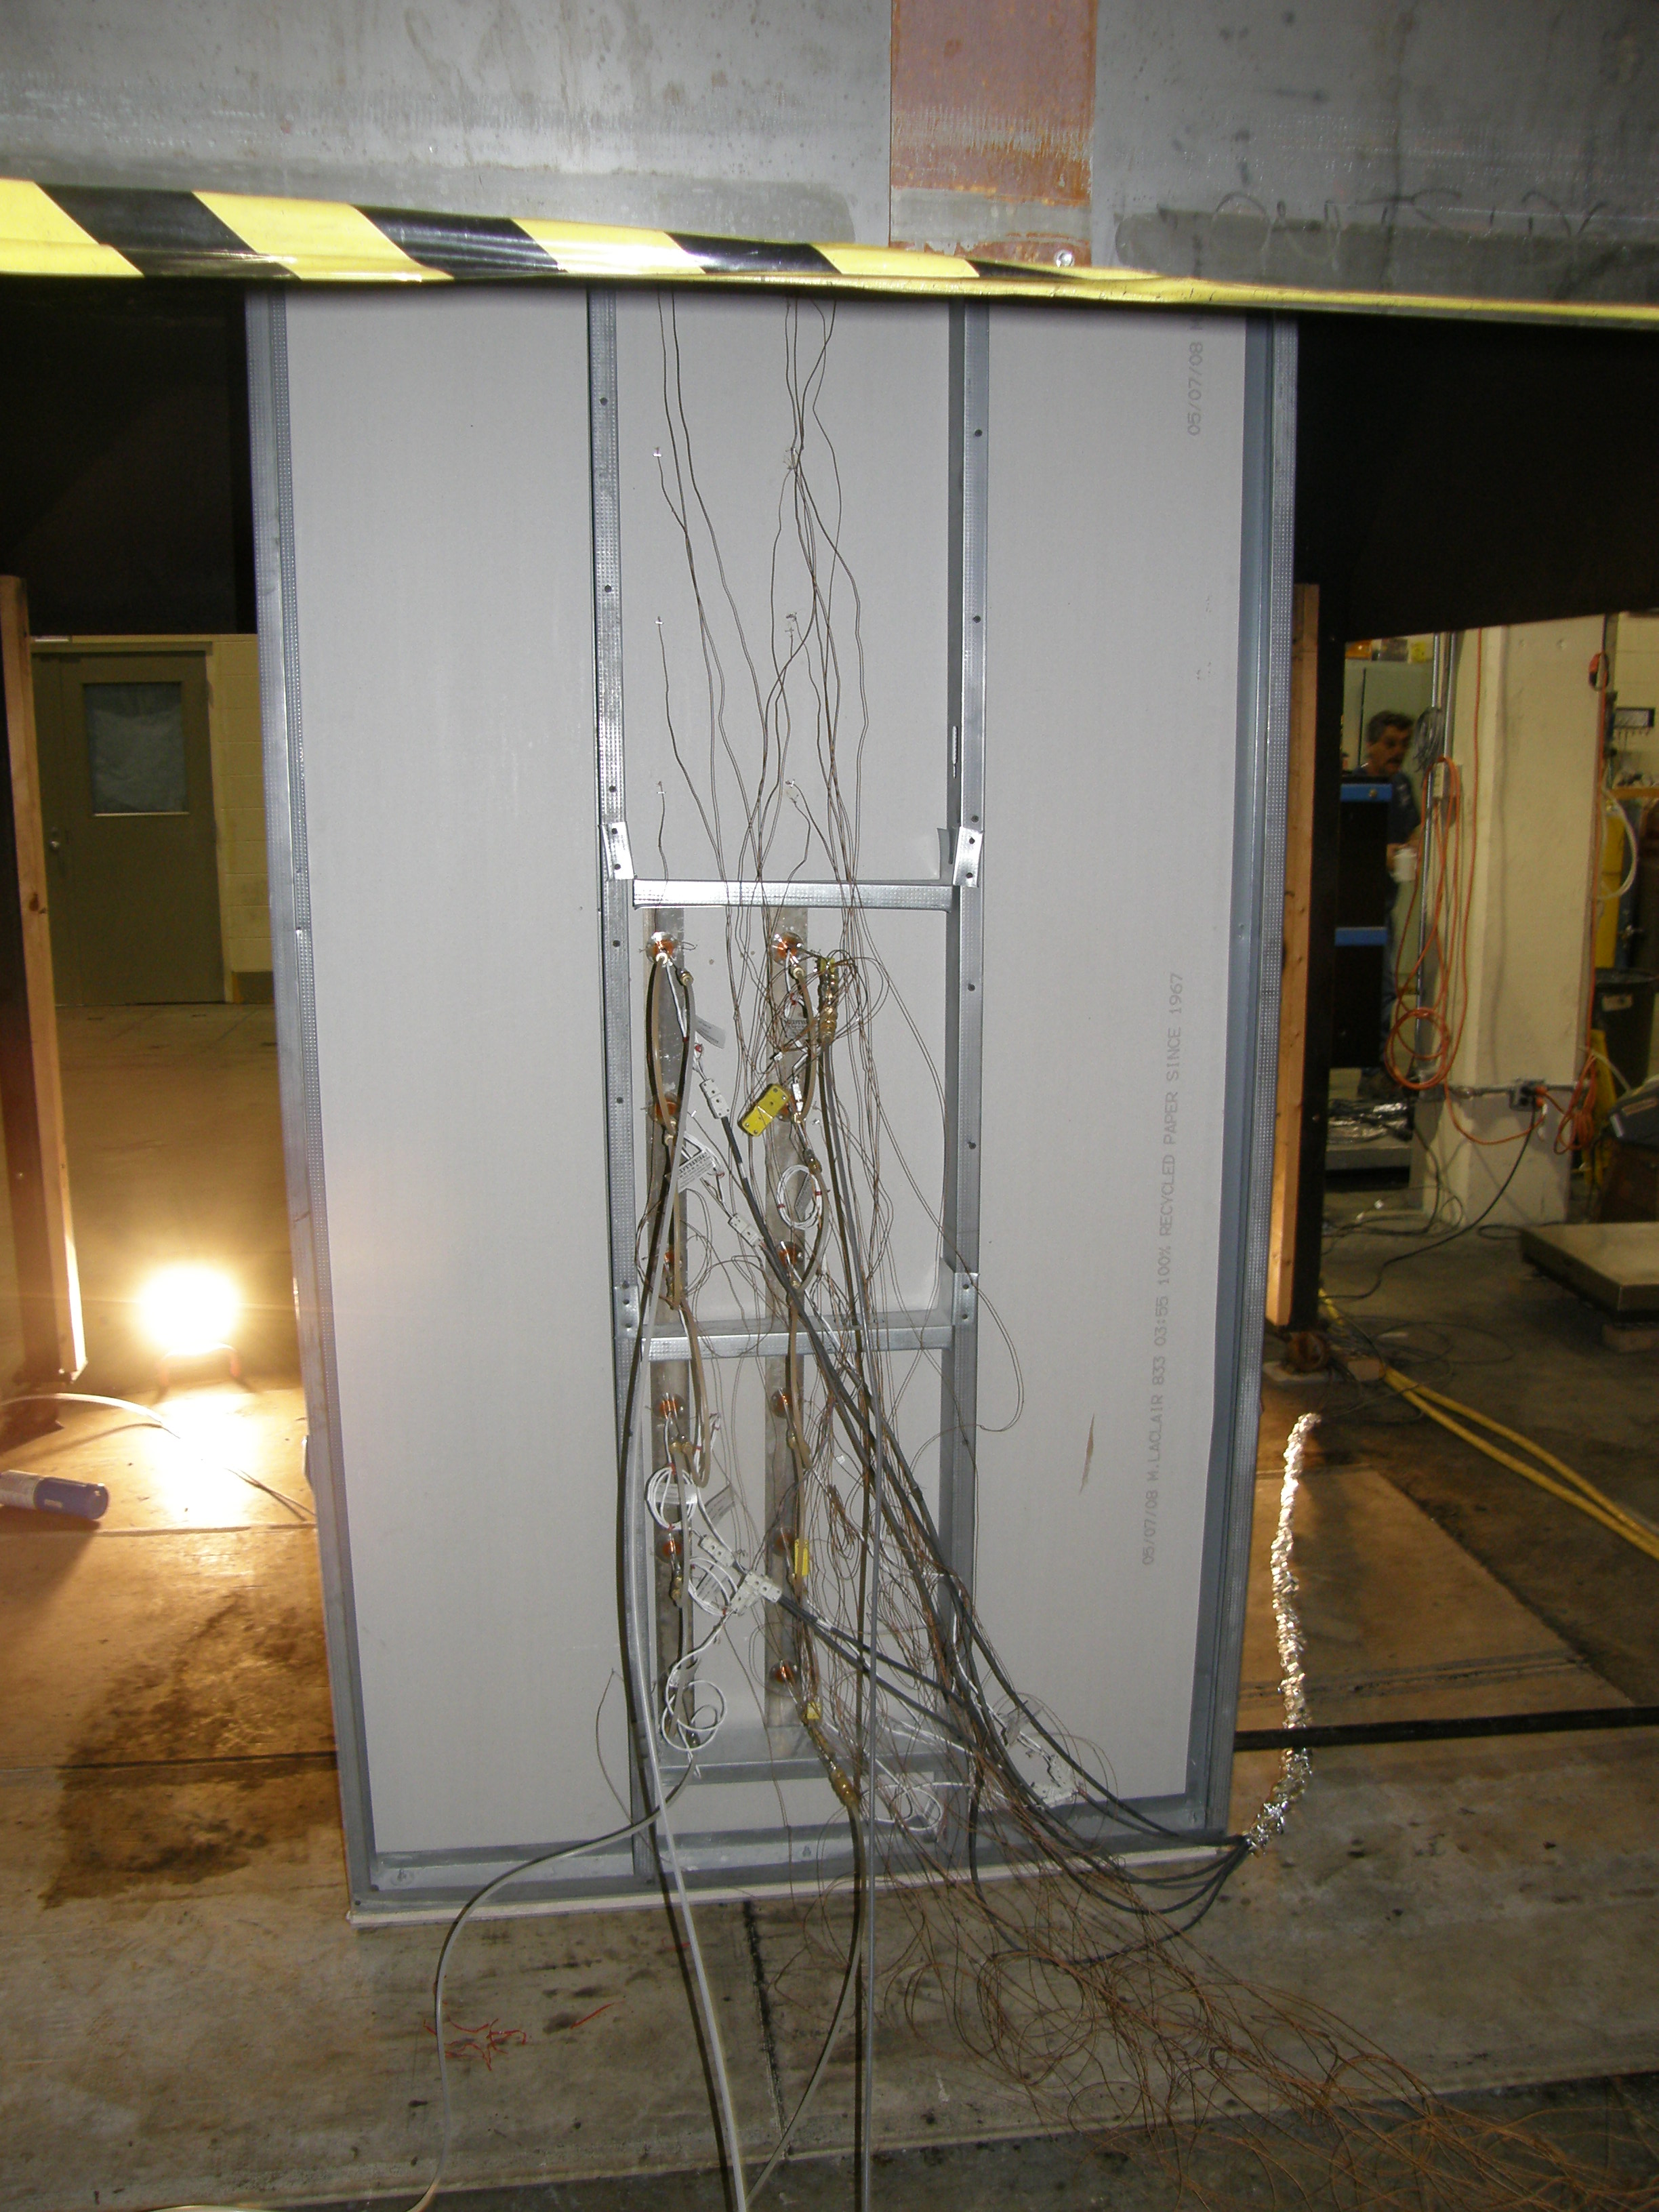
\includegraphics[width=\textwidth]{../Figures/Instrumented_Wall_Rear_photo}\\
	\caption[Photograph of the rear side of the instrumented non-combustible wall]{Photograph of the rear side of the instrumented non-combustible wall.}
	\label{Instrumented_Wall_Rear_photo}
\end{figure}

\begin{figure}
	\centering
	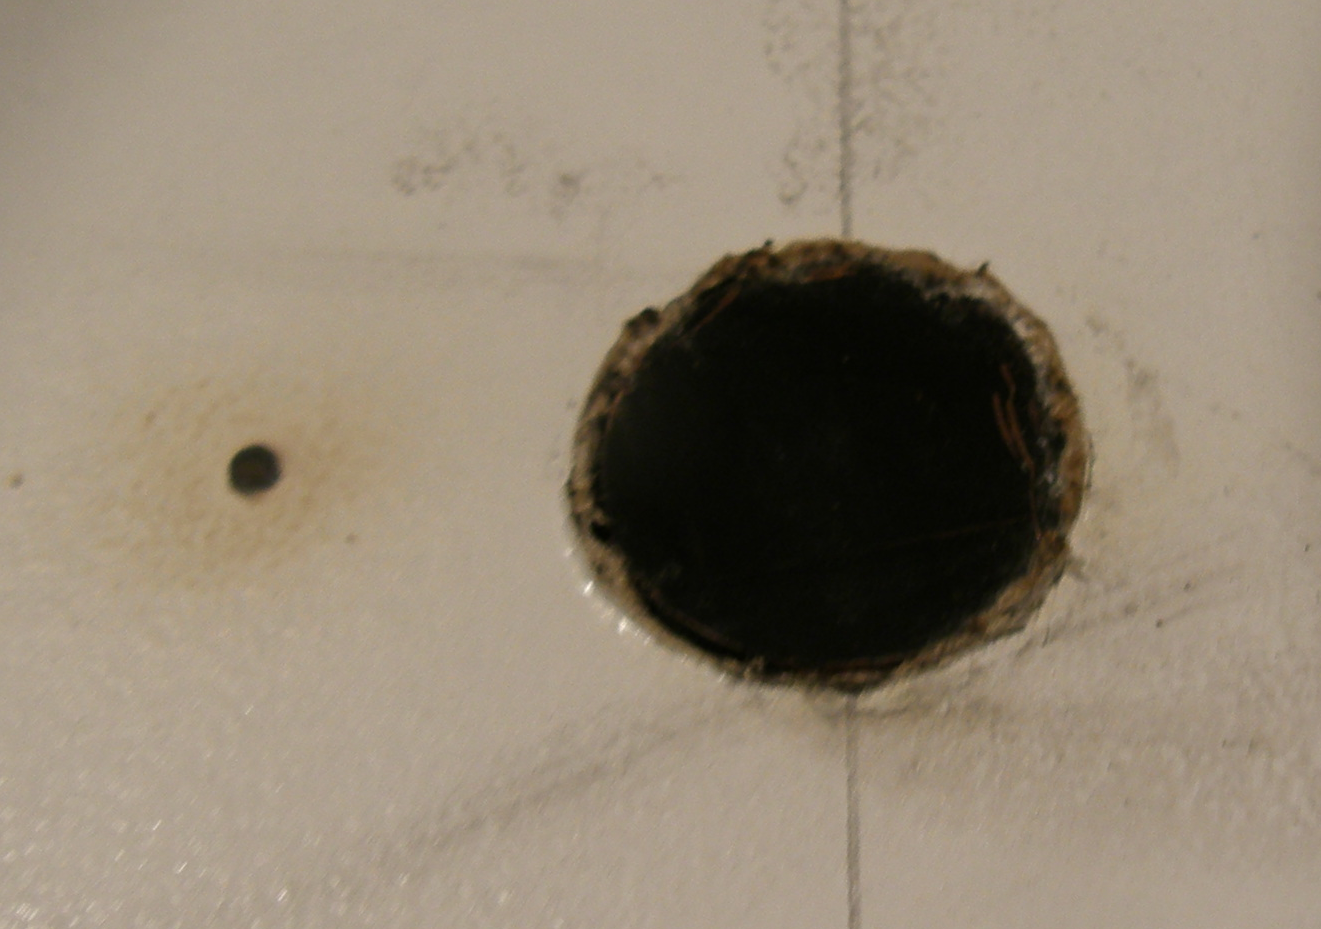
\includegraphics[width=4.0in]{../Figures/Instrumented_Wall_Close_up_TC_HF_photo}\\
	\caption[Photograph showing an example of the co-location of the heat flux gauges and the thermocouples on the front surface of the wall.]{Photograph showing an example of the co-location of the heat flux gauges and the thermocouples on the front surface of the wall.}
	\label{Instrumented_Wall_Close_up_TC_HF_photo}
\end{figure}

\begin{figure}
	\centering
	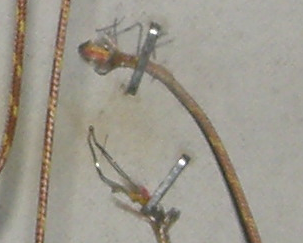
\includegraphics[width=4.0in]{../Figures/Instrumented_Wall_Detail_Rear_TC_photo}\\
	\caption[Photograph of an example of the co-location of the thermocouple on the rear surface of the wall relative to the thermocouple installed on the front surface of the wall]{Photograph of an example of the co-location of the thermocouple on the rear surface of the wall relative to the thermocouple installed on the front surface of the wall.}
	\label{Instrumented_Wall_Detail_Rear_TC_photo}
\end{figure}


\section{Results}

The results are presented for each of the four burner positions, (0.61~m, 0.31~m, 0.15~m and 0.0~m), and each of the three fuels in Appendix B.  For the natural gas fueled experiments only two replicates were conducted at each position given the higher level of control and repeatability.  For the gasoline and polyurethane fueled experiments, three replicates were conducted at each position. The position is measured as the distance between the edge of the burner closest to the wall and the wall.  The results of the wall temperatures and heat fluxes are presented as averages of the replicate experiments.  In the sections below, a full set of the averaged data from the natural gas fueled experiments will be presented to demonstrate the impact on distance from the wall on the temperatures in the plume as well as the conditions measured on the wall. Then composite graphs of the wall temperatures and heat flux measure on the wall versus distance will be shown for each fuel type.

Figures~\ref{TC_Plume_TWNG_comp} through \ref{TC_Back_Center_TWNG_comp} show a complete set of data, averaged over two replicates, for the instrumented, non combustible wall natural gas burner experiments.  Comparing the temperatures of the plume at the most distant point from the wall, 0.61~m and with the plume temperatures with the burner contacting the wall in Figure~\ref{TC_Plume_TWNG_comp} shows an increase.  However for the burner position, 0.15~m from the wall, a decrease in plume temperatures occurs after approximately 3~min after ignition.  A review of the heat release rates and the test videos do not yield any clues as to the reason for this decrease which occurred in both experiments.  In both experiments the heat release rate was steady and the video did not show any change in flame movement.
Figures~\ref{TC_Surf_Cent_TWNG_comp} and \ref{TC_Surf_Edge_TWNG_comp} show consistent trends of the thermocouple temperatures in the vertical arrays on the wall increasing as the burner was moved toward the wall.  Figure~\ref{TC_Back_Center_TWNG_comp} shows that the peak temperatures aligned with the vertical center of the burner on the backside of the gypsum wallboard peaked at approximately 100~$^\circ$C.


\begin{figure}[ht!]
	\centering
	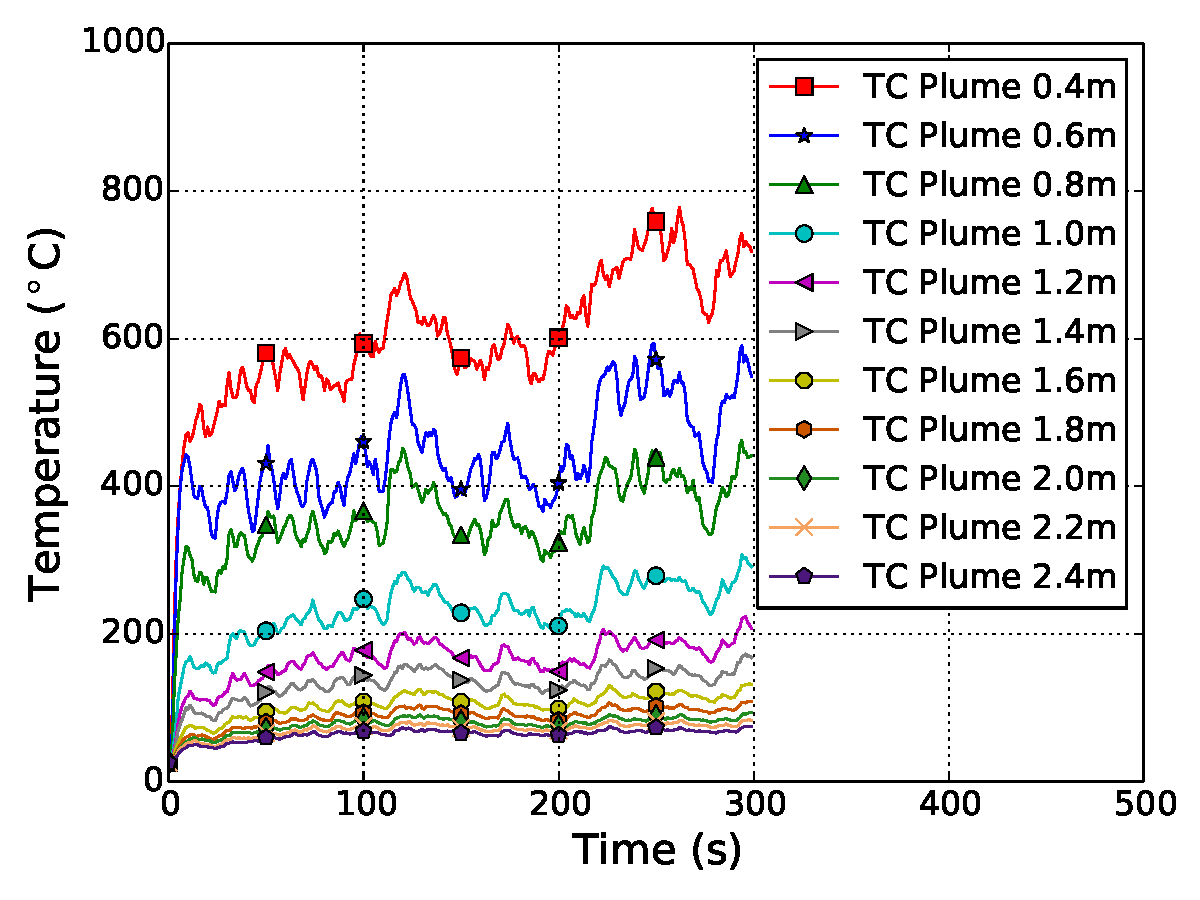
\includegraphics[width=2.5in]{../Figures/TWNG01_TC_Plume_Avg}
	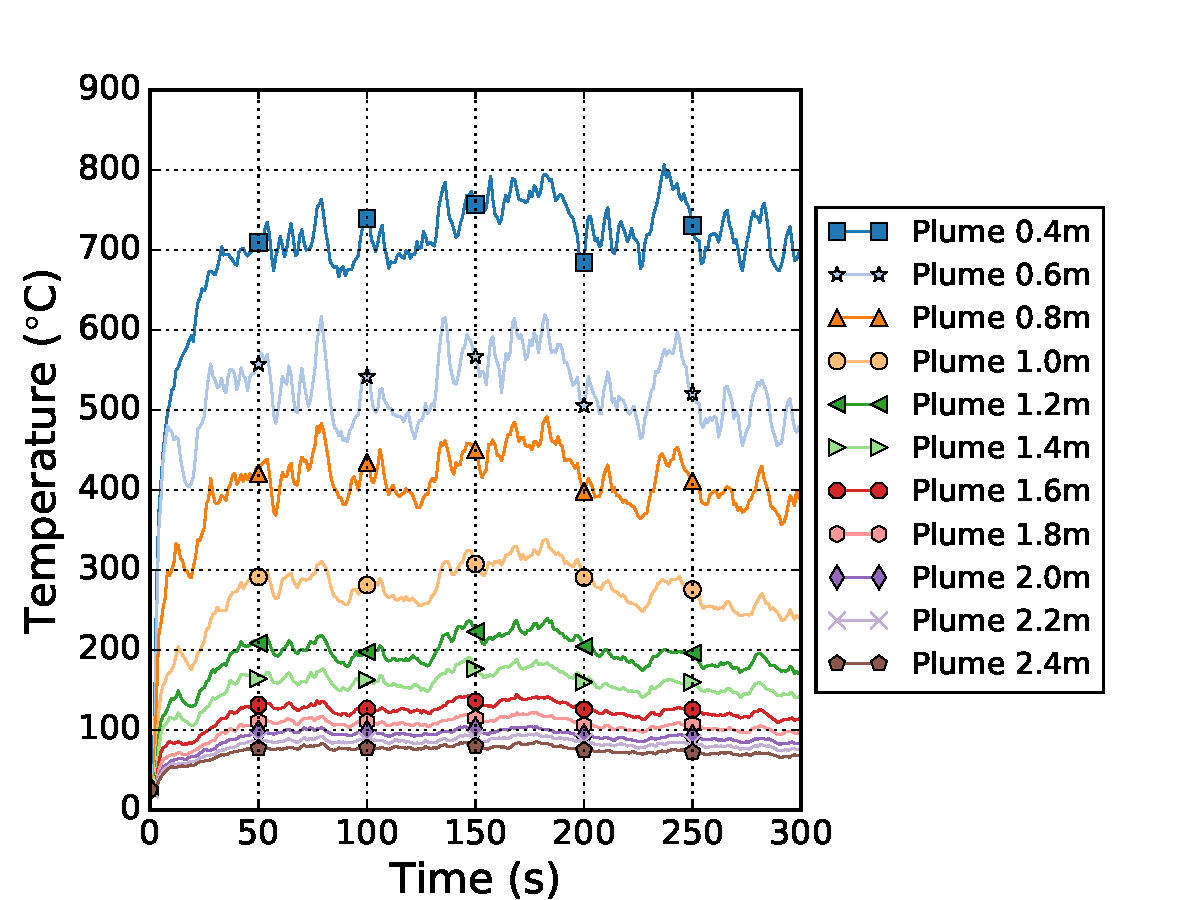
\includegraphics[width=2.5in]{../Figures/TWNG03_TC_Plume_Avg}\\
	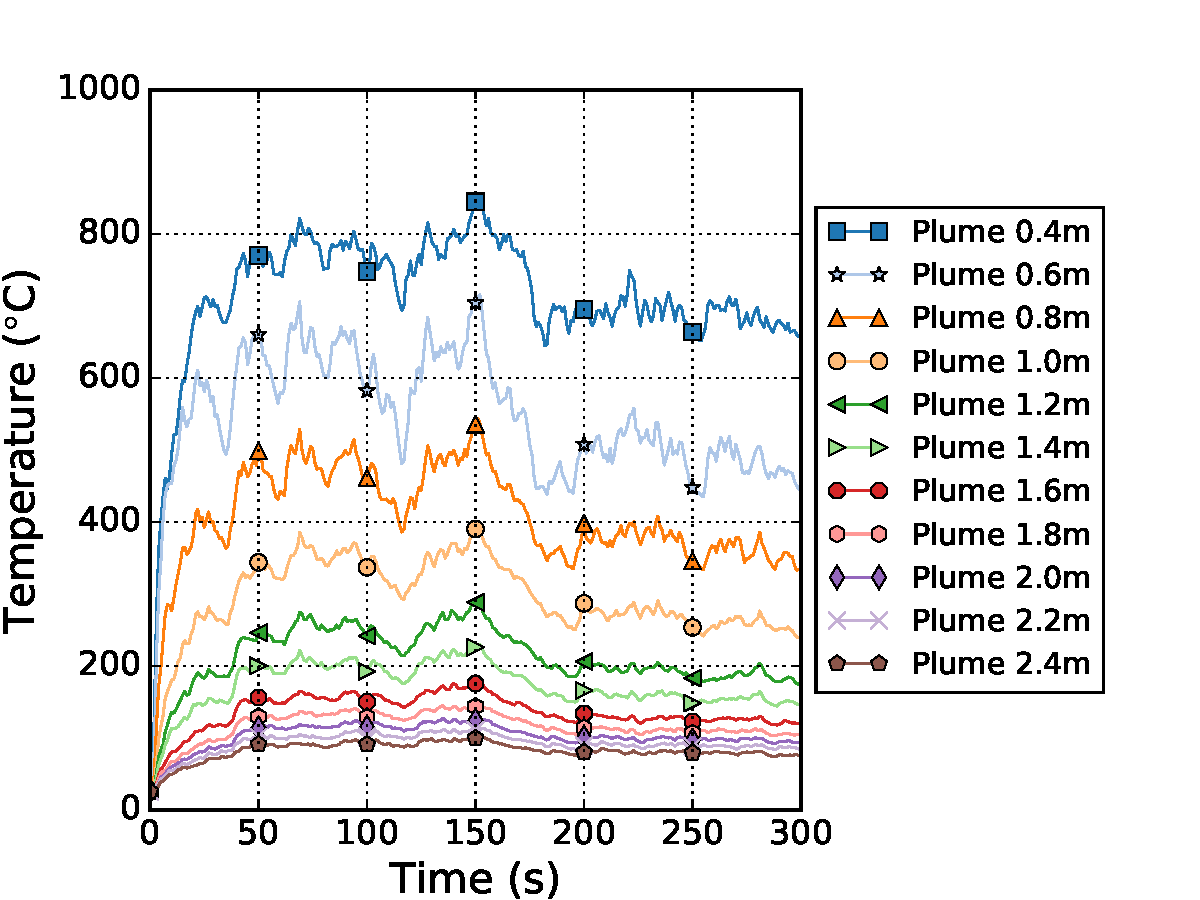
\includegraphics[width=2.5in]{../Figures/TWNG05_TC_Plume_Avg}
	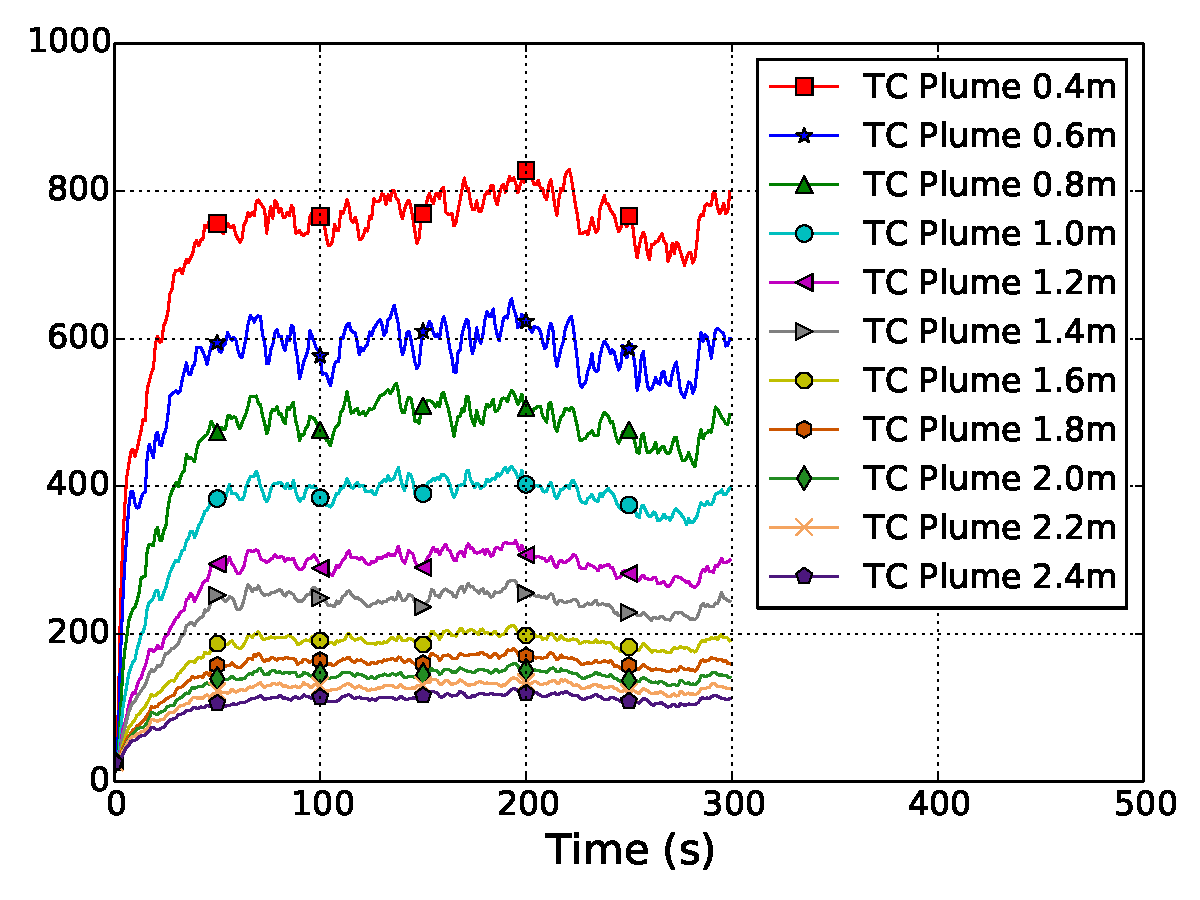
\includegraphics[width=2.5in]{../Figures/TWNG07_TC_Plume_Avg}\\
	\caption[Plume temperatures along the centerline of the natural gas fueled burner]{Plume temperatures along the centerline of the natural gas fueled burner. The temperatures are averages of two replicate experiments. Each graph displays data from a different distance between the edge of the burner and the instrumented wall.  Beginning with the top left graph position and viewing left to right the distances from the wall are 0.61~m, 0.31~m, 0.15~m, and 0~m respectively.}
	\label{TC_Plume_TWNG_comp}
\end{figure}

\begin{figure}[ht!]
	\centering
		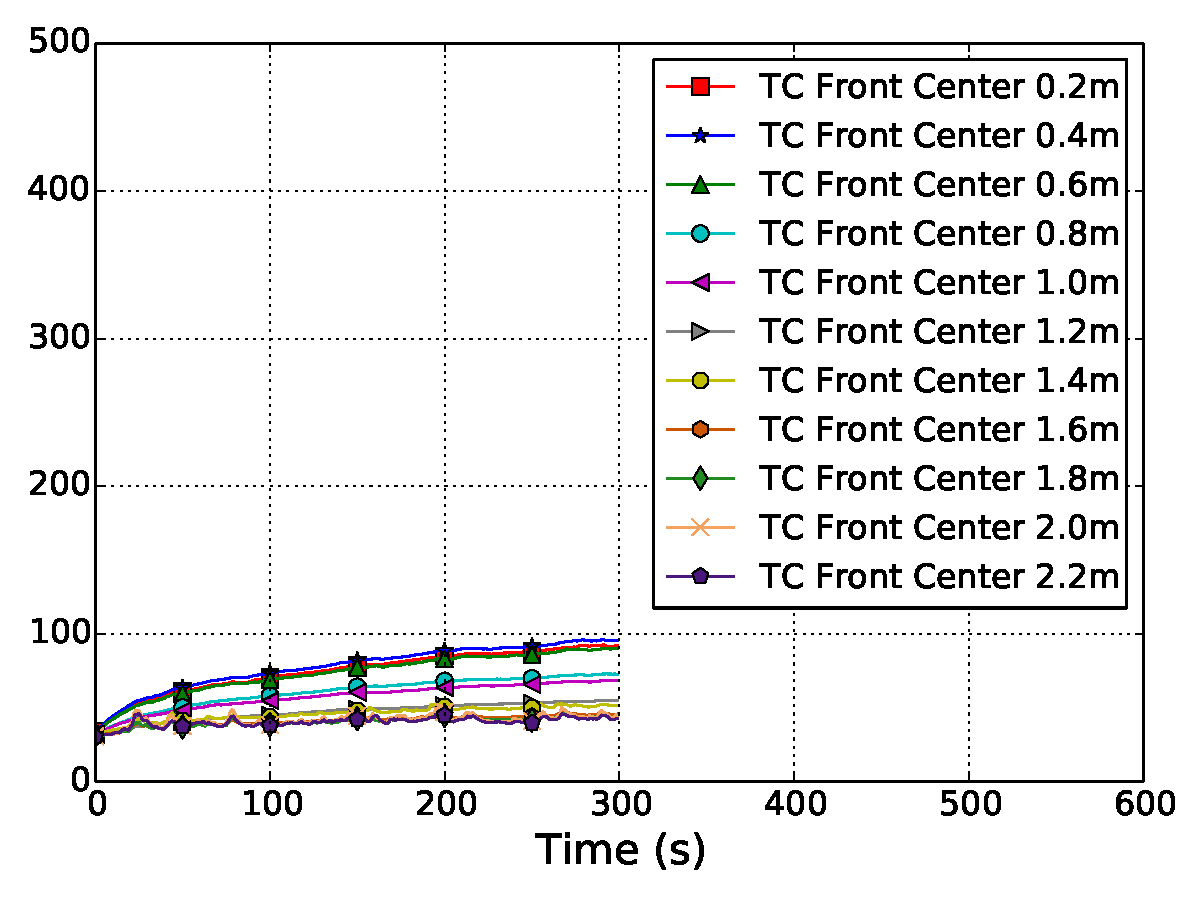
\includegraphics[width=2.5in]{../Figures/TWNG01_TC_Surface_Center_Avg}
		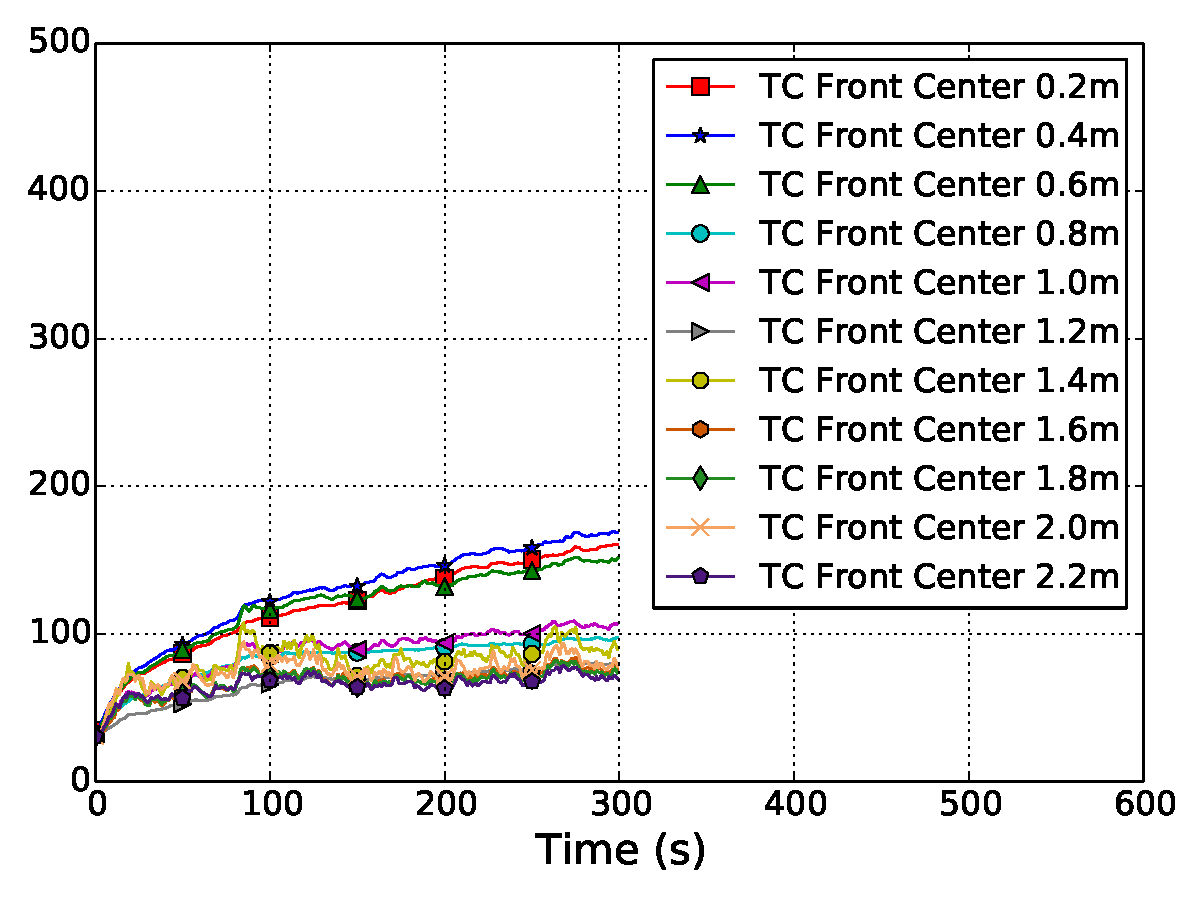
\includegraphics[width=2.5in]{../Figures/TWNG03_TC_Surface_Center_Avg}\\
		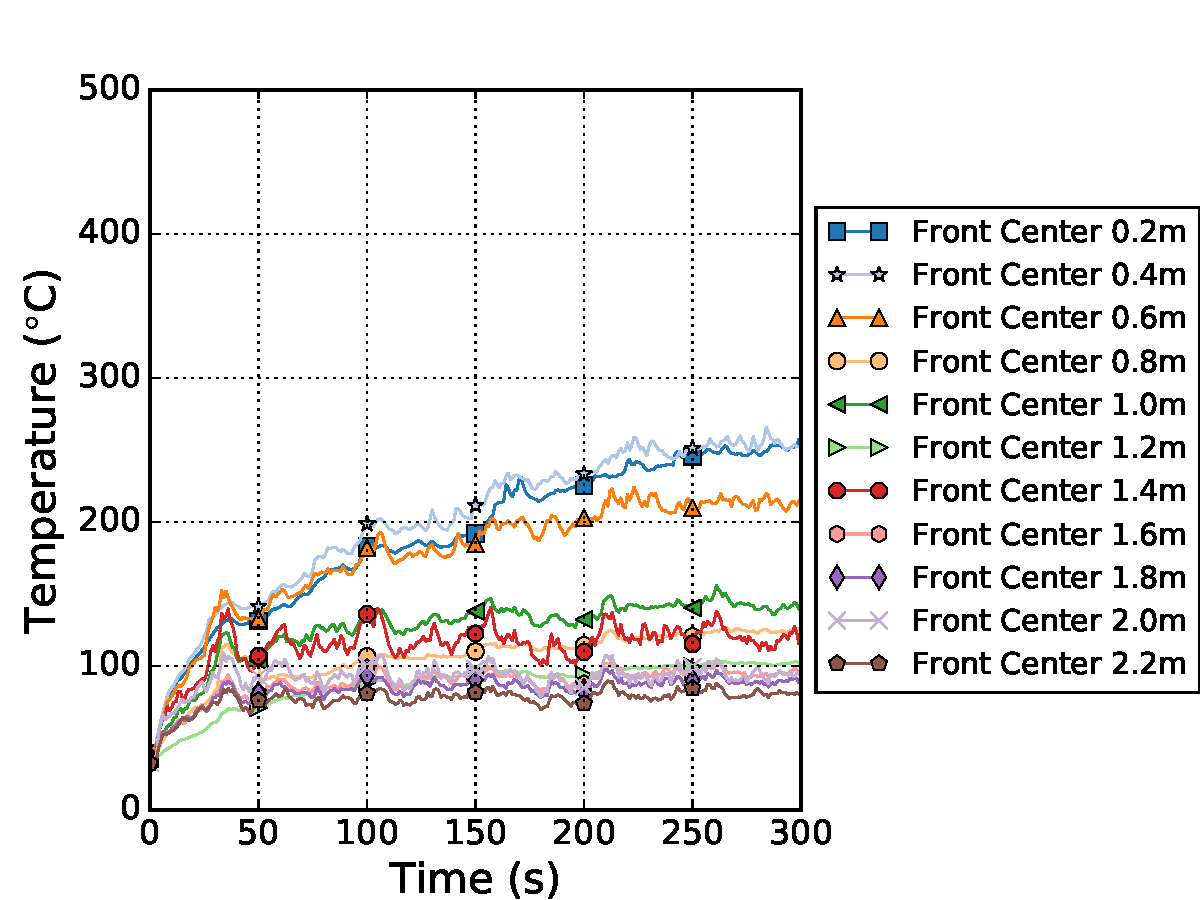
\includegraphics[width=2.5in]{../Figures/TWNG05_TC_Surface_Center_Avg}
		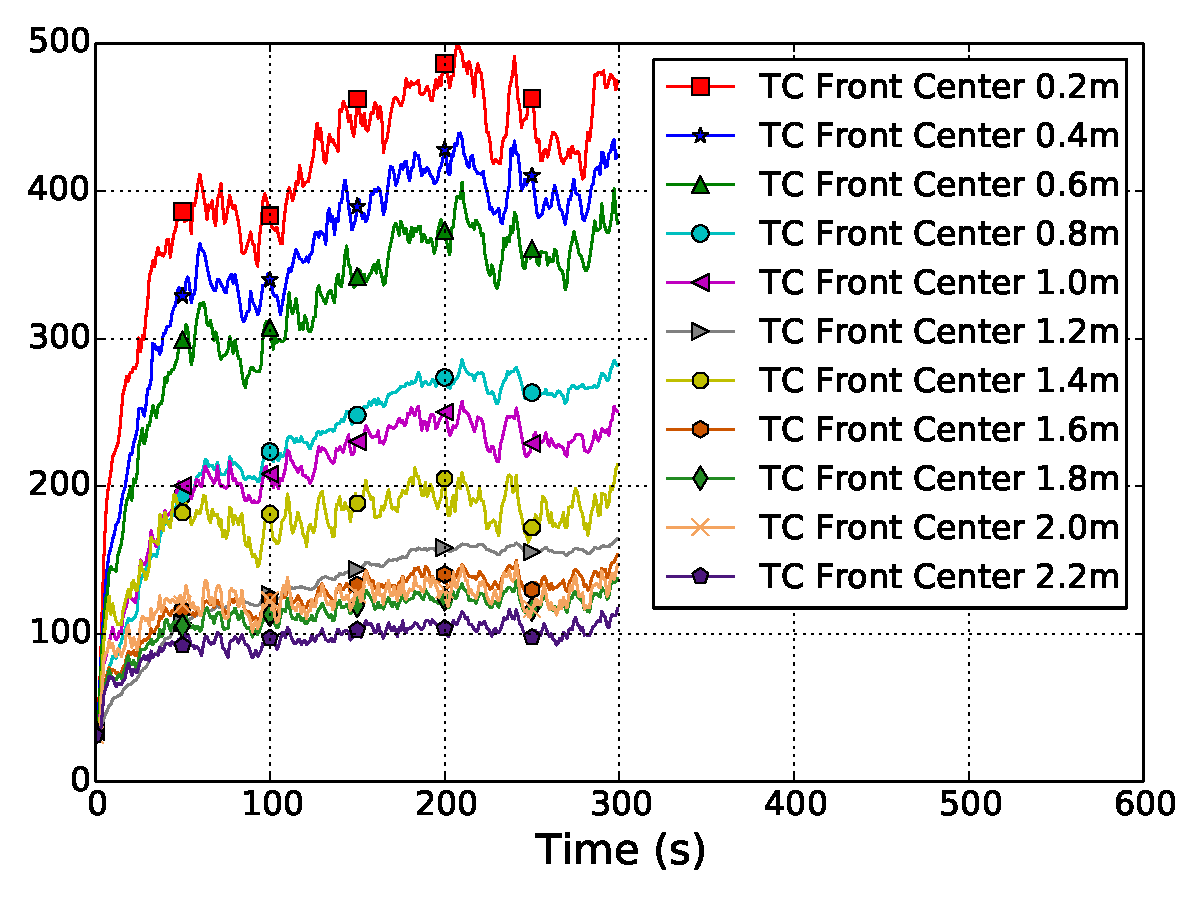
\includegraphics[width=2.5in]{../Figures/TWNG07_TC_Surface_Center_Avg}\\
	\caption[Wall Temperatures along the centerline of the natural gas fueled burner]{Wall Temperatures along the centerline of the natural gas fueled burner. The temperatures are averages of two replicate experiments. Each graph displays data from a different distance between the edge of the burner and the instrumented wall.  Beginning with the top left graph position and viewing left to right the distances from the wall are 0.61~m, 0.31~m, 0.15~m, and 0~m respectively.}
	\label{TC_Surf_Cent_TWNG_comp}
\end{figure}

\begin{figure}[ht!]
	\centering
	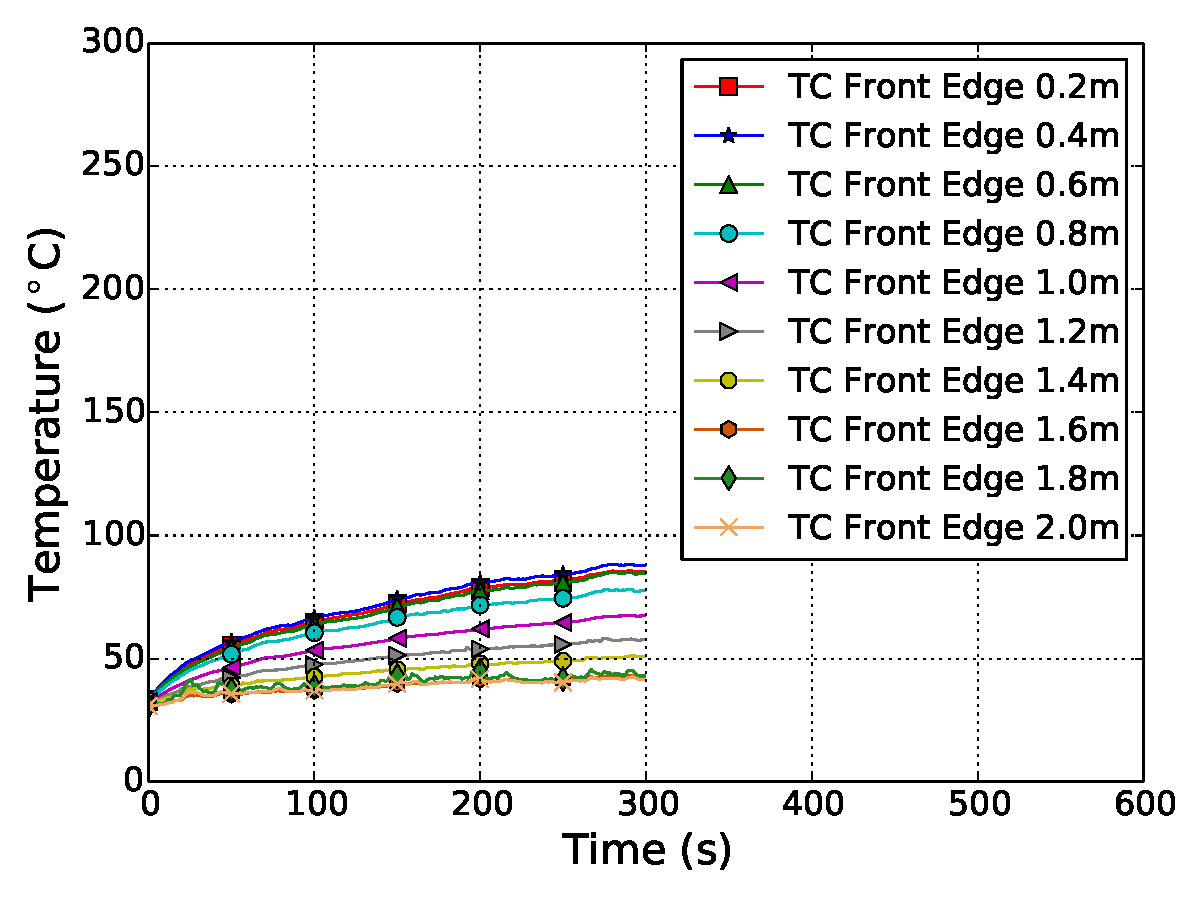
\includegraphics[width=2.5in]{../Figures/TWNG01_TC_Surface_Offset_Avg}
	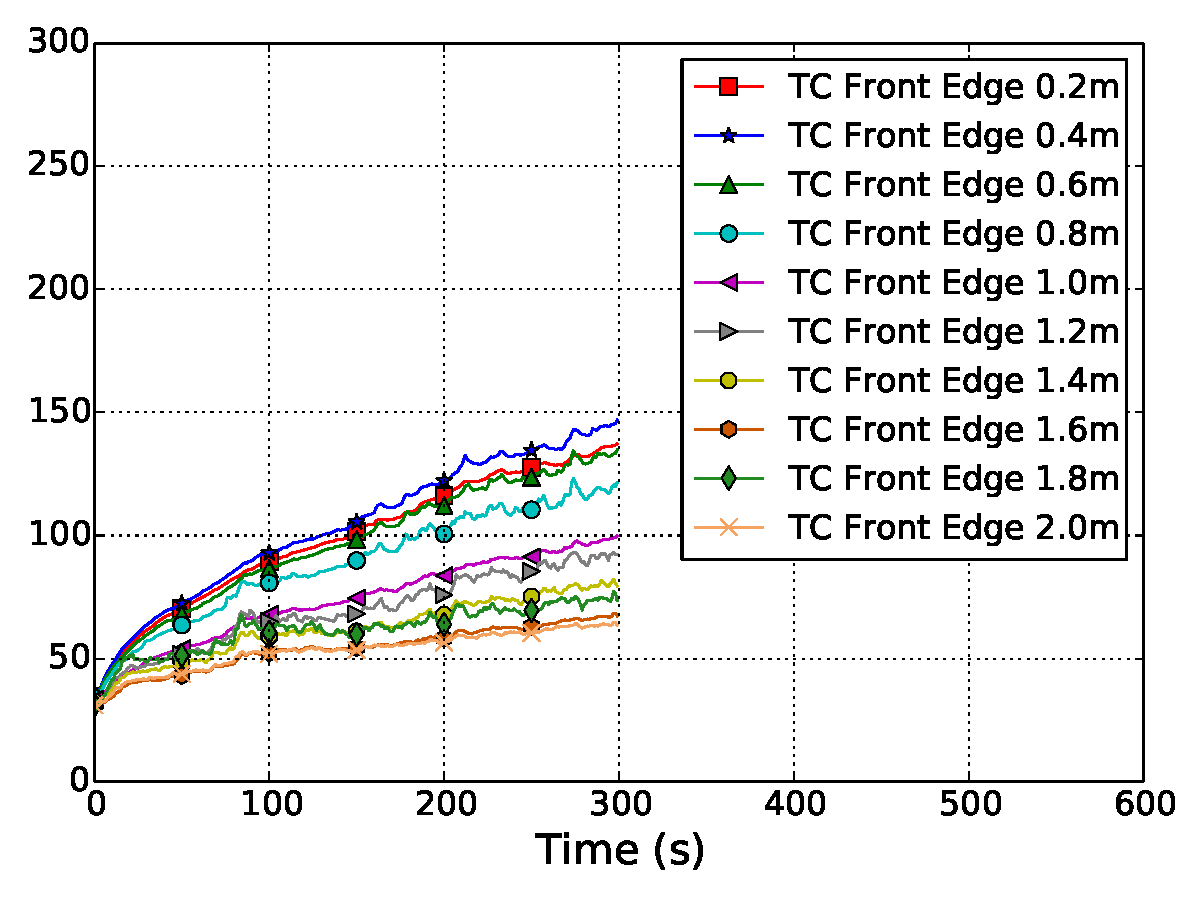
\includegraphics[width=2.5in]{../Figures/TWNG03_TC_Surface_Offset_Avg}\\
	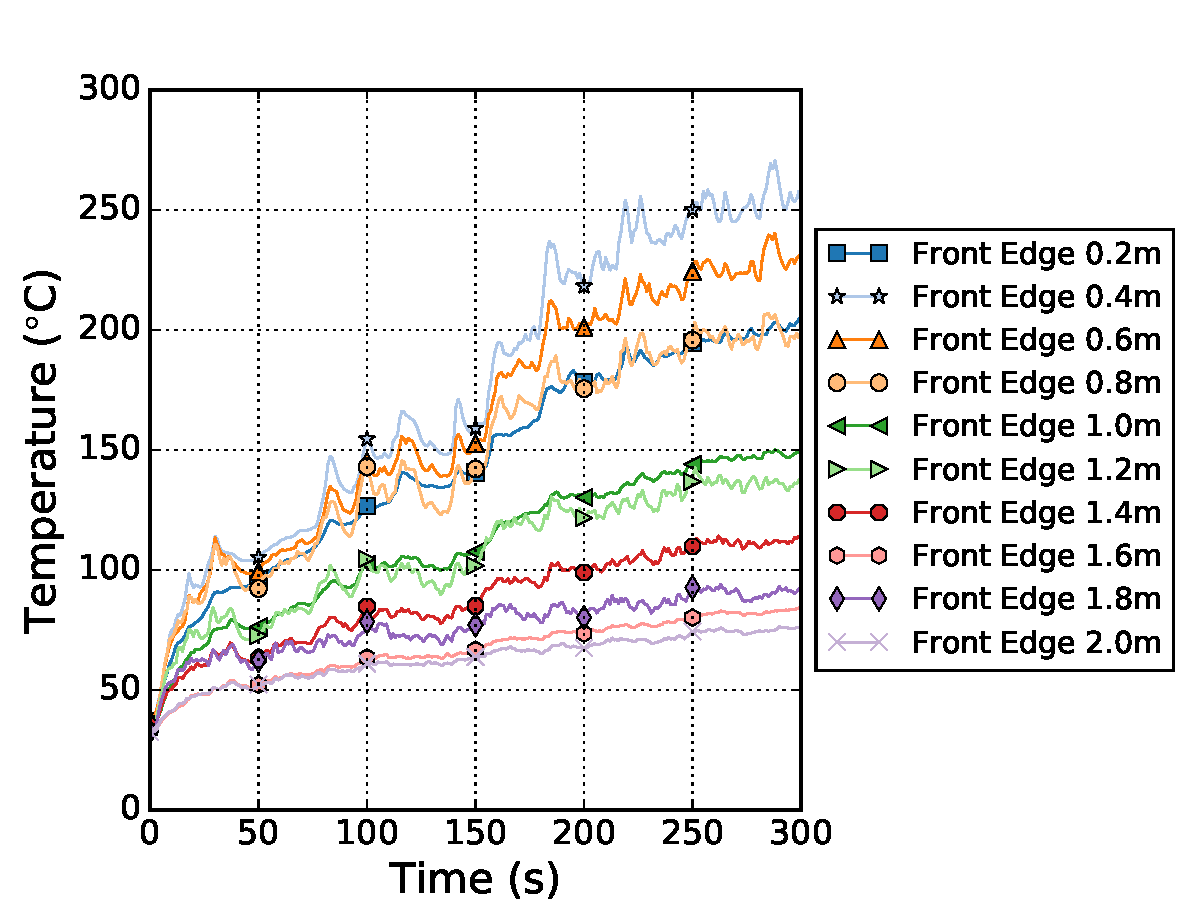
\includegraphics[width=2.5in]{../Figures/TWNG05_TC_Surface_Offset_Avg}
	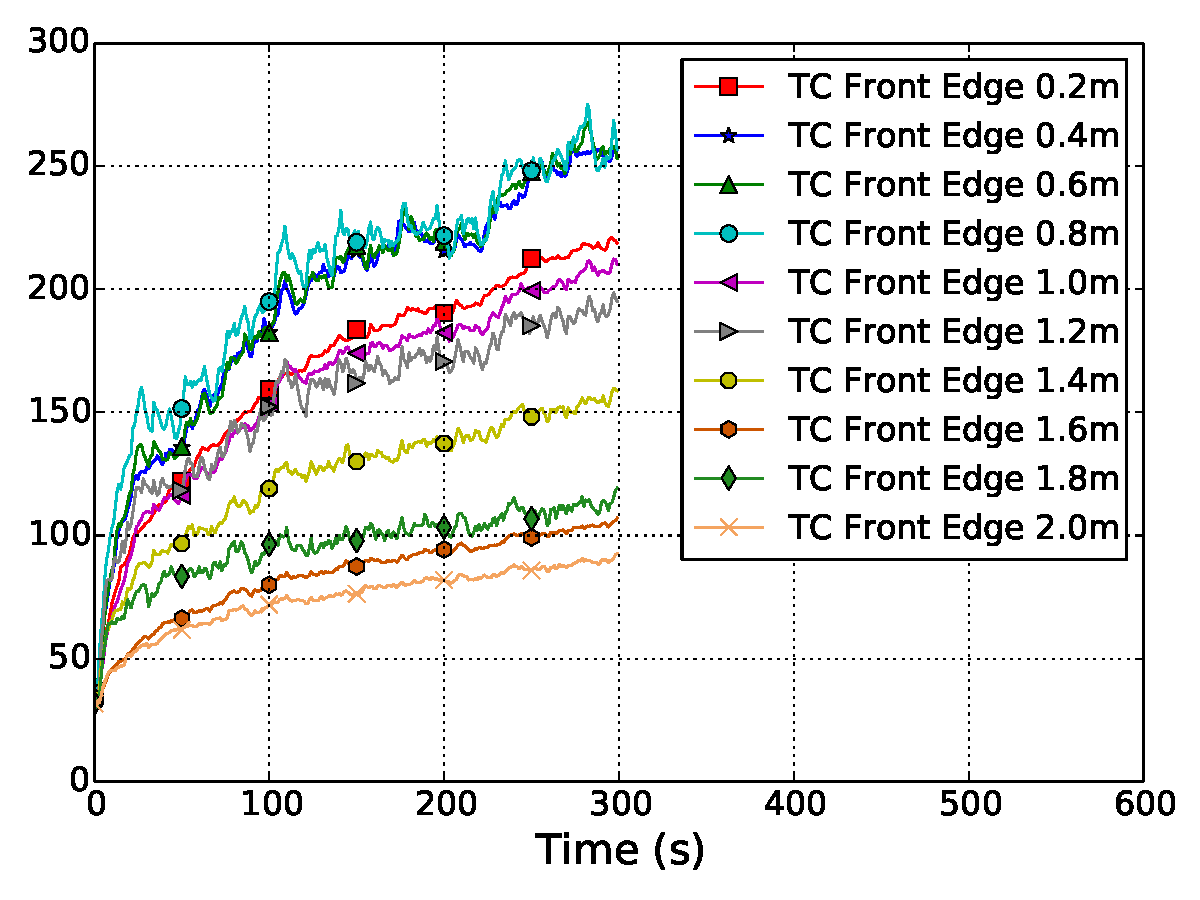
\includegraphics[width=2.5in]{../Figures/TWNG07_TC_Surface_Offset_Avg}\\
	\caption[Wall Temperatures along the edge of the natural gas fueled burner]{Wall Temperatures along the right edge of the natural gas fueled burner, when facing the wall. The temperatures are averages of two replicate experiments. Each graph displays data from a different distance between the edge of the burner and the instrumented wall.  Beginning with the top left graph position and viewing left to right the distances from the wall are 0.61~m, 0.31~m, 0.15~m, and 0~m respectively.}
	\label{TC_Surf_Edge_TWNG_comp}
\end{figure}

\begin{figure}[ht!]
	\centering
	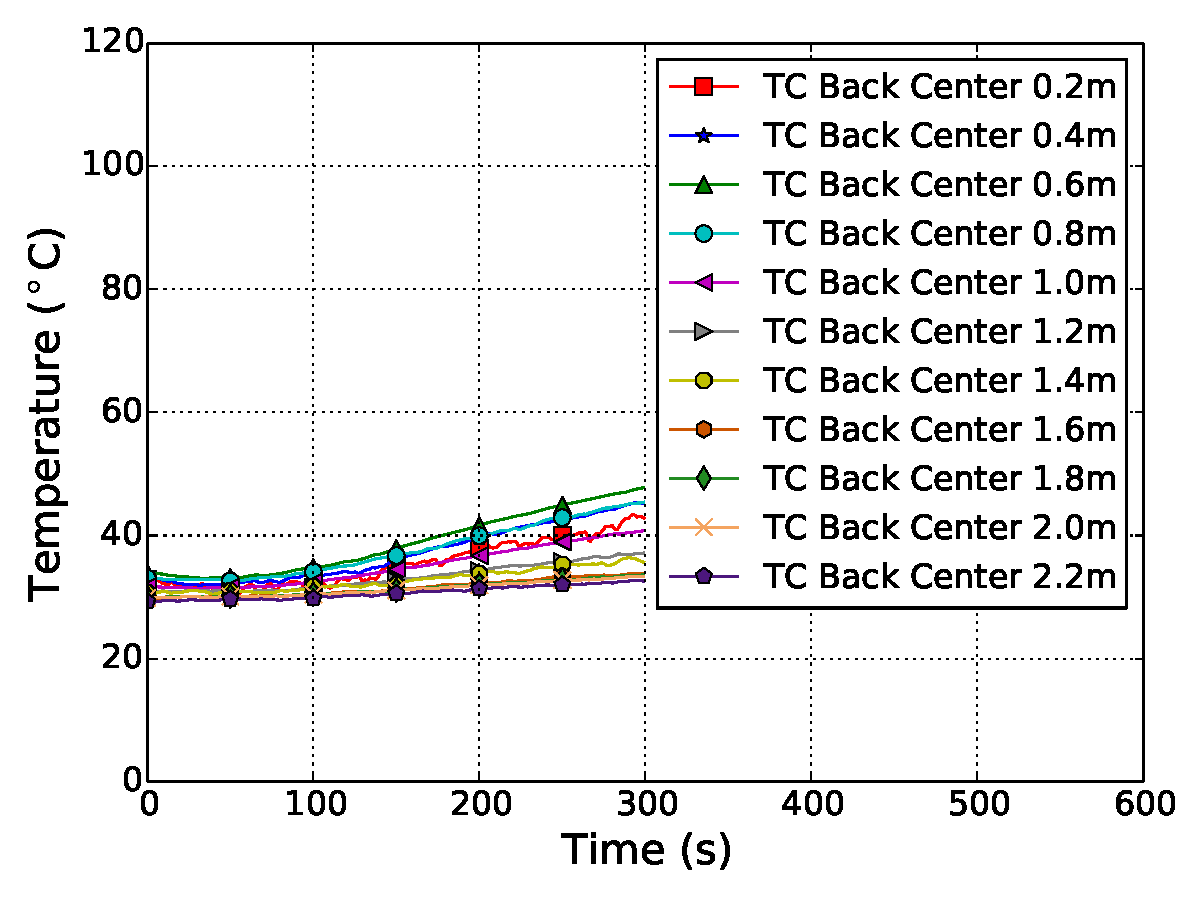
\includegraphics[width=2.5in]{../Figures/TWNG01_TC_Back_Center_Avg}
	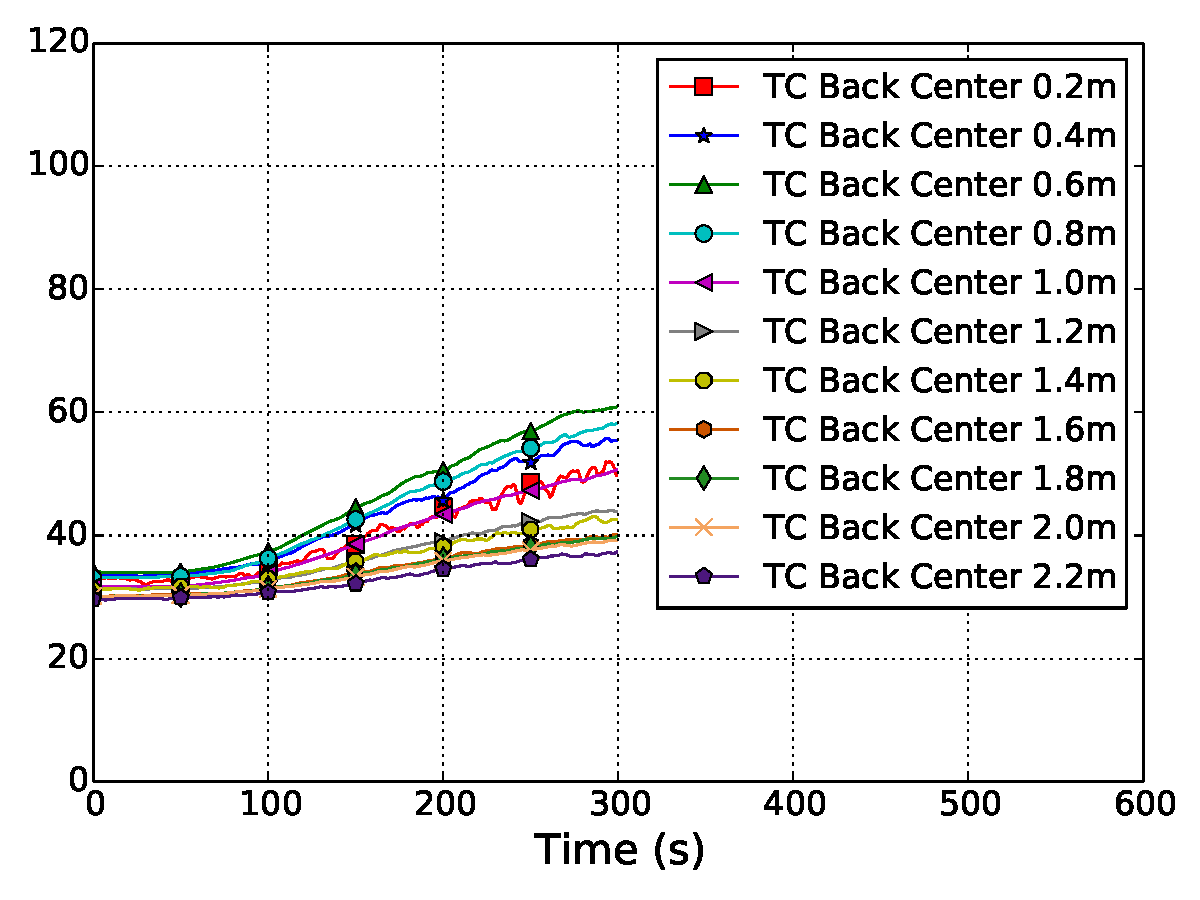
\includegraphics[width=2.5in]{../Figures/TWNG03_TC_Back_Center_Avg}\\
	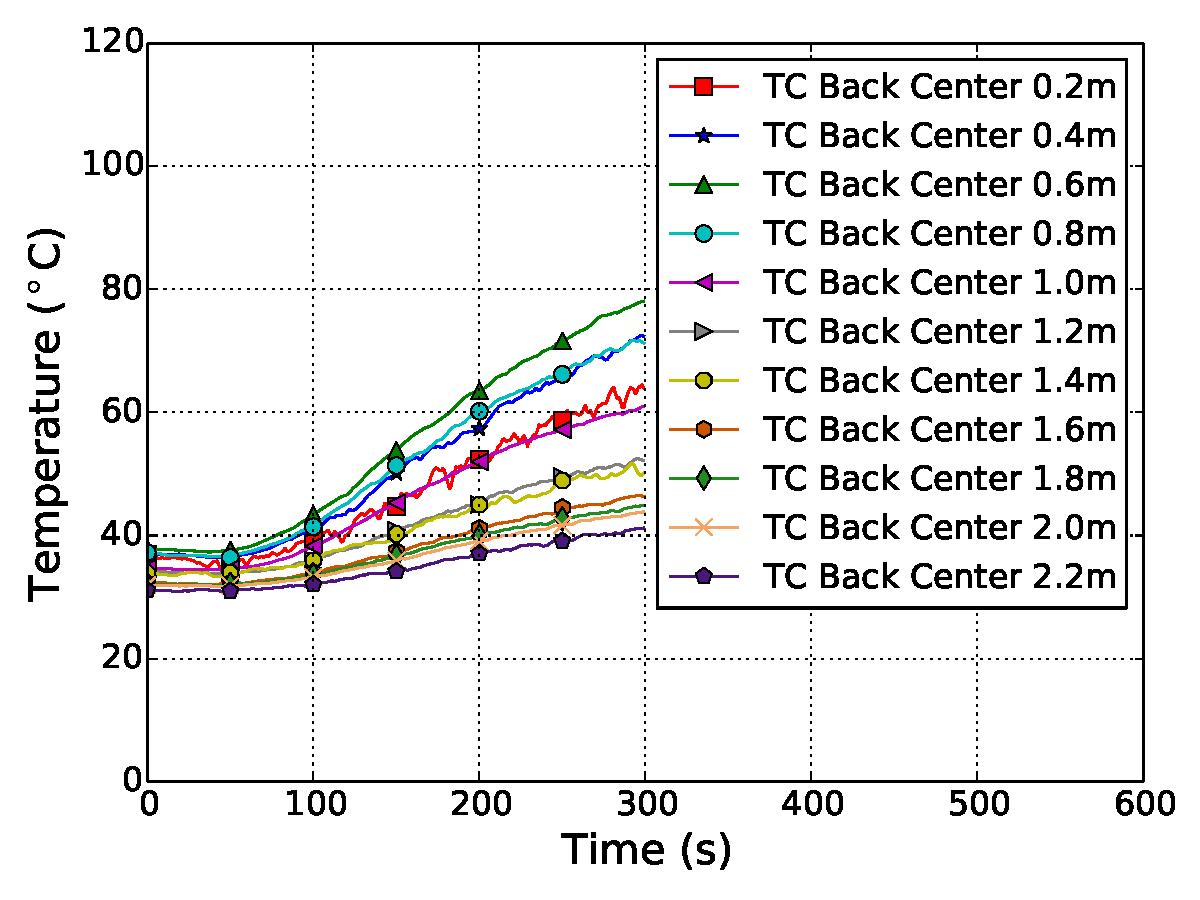
\includegraphics[width=2.5in]{../Figures/TWNG05_TC_Back_Center_Avg}
	\includegraphics[width=2.5in]{../Figures/TWNG07_TC_Back_Center_Avg}\\
	\caption[Backside wall Temperatures along the centerline of the natural gas fueled burner]{Backside wall Temperatures along the centerline of the natural gas fueled burner. The temperatures are averages of two replicate experiments. Each graph displays data from a different distance between the edge of the burner and the instrumented wall. Beginning with the top left graph position and viewing left to right the distances from the wall are 0.61~m, 0.31~m, 0.15~m, and 0~m respectively.}
	\label{TC_Back_Center_TWNG_comp}
\end{figure}

Figures~\ref{HF_Center_TWNG_comp} and \ref{HF_Edge_TWNG_comp} provide the heat flux measurements for the two vertical arrays of gauges positioned along the centerline and the edge of the natural gas burner.  The series of graphs show that the peak heat flux increases as the burner is moved toward the wall. One exception is when the burner was moved from the 0.15~m position to the 0.0~m from the wall. In this comparison the peak heat flux values for the gauges located above the edge of the burner do not uniformly increase.  In fact the peak heat flux actually decreased as the burner was moved from the 0.15~m position to the 0.0~m position. This decrease was due to the change in view angle between the flame closest to the burner and the lower heat flux gauges at the edge of the burner.

\begin{figure}[ht!]
	\centering
	\includegraphics[width=2.5in]{../Figures/TWNG01_HF_Center_Avg}
	\includegraphics[width=2.5in]{../Figures/TWNG03_HF_Center_Avg}\\
	\includegraphics[width=2.5in]{../Figures/TWNG05_HF_Center_Avg}
	\includegraphics[width=2.5in]{../Figures/TWNG07_HF_Center_Avg}\\
	\caption[Heat flux at the wall along the centerline of the natural gas fueled burner]{Heat flux at the wall along the centerline of the natural gas fueled burner. The heat fluxes are averages of two replicate experiments. Each graph displays data from a different distance between the edge of the burner and the instrumented wall. Beginning with the top left graph position and viewing left to right the distances from the wall are 0.61~m, 0.31~m, 0.15~m, and 0~m respectively.}
	\label{HF_Center_TWNG_comp}
\end{figure}


\begin{figure}[ht!]
	\centering
	\includegraphics[width=2.5in]{../Figures/TWNG01_HF_Offset_Avg}
	\includegraphics[width=2.5in]{../Figures/TWNG03_HF_Offset_Avg}\\
	\includegraphics[width=2.5in]{../Figures/TWNG05_HF_Offset_Avg}
	\includegraphics[width=2.5in]{../Figures/TWNG07_HF_Offset_Avg}\\
	\caption[Heat flux at the wall along the edge of the natural gas fueled burner]{Heat flux at the wall along the edge of the natural gas fueled burner. The heat fluxes are averages of two replicate experiments. Each graph displays data from a different distance between the edge of the burner and the instrumented wall. Beginning with the top left graph position and viewing left to right the distances from the wall are 0.61~m, 0.31~m, 0.15~m, and 0~m respectively.}
	\label{HF_Edge_TWNG_comp}
\end{figure}

In the following sections, the data is compiled so that averaged peak values, of a given measure, for each position from the wall will be presented on a single graph for a given fuel type.

\subsection{Wall Temperatures}

Figure~\ref{NCTW_Surf_Center_comp} shows the wall temperatures based on the array of thermocouples installed in the wall and position along the vertical centerline of the burners for each of the three fuels. Reviewing the graph for each fuel demonstrates how the temperature at the wall decreased as the position of the burner increased from the wall. The beads of the thermocouples were installed in the wall and were flush with the wall surface. In each graph, the average peak temperature of the replicate experiments, for each thermocouple position is shown. Moving from 0.2~m above the top surface of the burner up to 2.2~m above the top of the burner surface in increments of 0.2~m. As with the data analysis for the source fires, the peak averages were based on a 30~s period bounding the peak for the natural gas and gasoline fires.  A 15~s interval bounding the peak was used for the polyurethane, in order to be more representative of the peak conditions.

Figure~\ref{NCTW_Surf_Edge_comp} presents the temperature of the vertical array of thermocouples positioned on the wall along the edge of the burner for each of the three fuels.  The data is treated in the same manner as in Figure~\ref{NCTW_Surf_Center_comp}.  For each fuel the average peak temperatures at the burner edge are significantly lower when the centerline temperatures when the burner is positioned against the wall.  As the burners were moved away from the wall the temperatures at the centerline and the edge thermocouple arrays begin to converge.

Temperatures were also measured on the backside of the wall, along the vertical centerline of the burners, Figure~\ref{NCTW_Back_Cent_comp}. The temperature difference between the peak average temperatures on the front (fire side) of the wall at 0.2~m above the burner vs the corresponding temperatures on the backside of the wall have a difference of at least 400~$^\circ$C.  It is consistent with the temperature data shown in Figures~\ref{NCTW_Surf_Center_comp} and \ref{NCTW_Surf_Edge_comp}, that as the burners were moved away from the wall the temperature differences are reduced.

\begin{figure}[p]
	\centering
	\includegraphics[width=3.5in]{../Figures/NCTW_NG_TC_Surface_Center_Avg}\\
	\includegraphics[width=3.5in]{../Figures/NCTW_GAS_TC_Surface_Center_Avg}\\
	\includegraphics[width=3.5in]{../Figures/NCTW_PUF_TC_Surface_Center_Avg}\\
	\caption[Composite graph of the wall temperatures along the centerline of the burners]{Composite graph of the wall temperatures along the centerline of the burners for each fuel. The peak temperatures are averages of replicate experiments for each instrument location at each position from the wall. Beginning with the top graph position and moving down the graph for natural gas, gasoline, and polyurethane foam are presented.}
	\label{NCTW_Surf_Center_comp}
\end{figure}

\begin{figure}[p]
	\centering
	\includegraphics[width=3.5in]{../Figures/NCTW_NG_TC_Surface_Offset_Avg}\\
	\includegraphics[width=3.5in]{../Figures/NCTW_GAS_TC_Surface_Offset_Avg}\\
	\includegraphics[width=3.5in]{../Figures/NCTW_PUF_TC_Surface_Offset_Avg}\\
	\caption[Composite graph of the wall temperatures along the edge of the burners]{Composite graph of the wall temperatures along the edge of the burners for each fuel. The peak temperatures are averages of replicate experiments for each instrument location at each position from the wall. Beginning with the top graph position and moving down, the graphs for natural gas, gasoline, and polyurethane foam are presented.}
	\label{NCTW_Surf_Edge_comp}
\end{figure}


\begin{figure}[p]
	\centering
	\includegraphics[width=3.5in]{../Figures/NCTW_NG_TC_Back_Center_Avg}\\
	\includegraphics[width=3.5in]{../Figures/NCTW_GAS_TC_Back_Center_Avg}\\
	\includegraphics[width=3.5in]{../Figures/NCTW_PUF_TC_Back_Center_Avg}\\
	\caption[Composite graph of the backside wall temperatures along the center of the burners]{Composite graph of the backside wall temperatures along the vertical centerline of the burners for each fuel. The peak temperatures are averages of replicate experiments for each instrument location at each position from the wall. Beginning with the top graph position and moving down, the graphs for natural gas, gasoline, and polyurethane foam are presented.}
	\label{NCTW_Back_Cent_comp}
\end{figure}


\subsection{Heat Flux}

Figures~\ref{NCTW_HF_Center_Comp} and \ref{NCTW_HF_Edge_Comp} show the results from the arrays of total heat flux gauges located along the vertical centerline and the edge of the burners for each fuel.  The sensing surface of the gauges were installed flush with the wall surface and exposed to the fire. In each graph, the averaged peak heat flux for each of the replicate experiments and each position is shown.  Moving from 0.2~m above the top surface of the burner up to 1.2~m above the top of the burner surface in increments of 0.2~m.  Reviewing the graph for each fuel demonstrates how the heat flux at the wall decreased as the position of the burner was moved away from the wall.  (Review video and tie in ST TC graph with edge peak NG at 0.15)

\begin{figure}[p]
	\centering
	\includegraphics[width=3.5in]{../Figures/NCTW_NG_HF_Center_Avg} \\
	\includegraphics[width=3.5in]{../Figures/NCTW_GAS_HF_Center_Avg}\\
	\includegraphics[width=3.5in]{../Figures/NCTW_PUF_HF_Center_Avg} \\
	\caption[Wall heat flux along the centerline of the burners]{Wall heat fluxes along the centerline of the burners.  The heat fluxes are averages of replicate experiments. Each graph displays data from a different distance between the edge of the burner and the instrumented wall.  Beginning with the top graph position and moving down, the graphs for natural gas, gasoline, and polyurethane foam are presented.}
	\label{NCTW_HF_Center_Comp}
\end{figure}

\begin{figure}[p]
	\centering
	\includegraphics[width=3.5in]{../Figures/NCTW_NG_HF_Offset_Avg} \\
	\includegraphics[width=3.5in]{../Figures/NCTW_GAS_HF_Offset_Avg}\\
	\includegraphics[width=3.5in]{../Figures/NCTW_PUF_HF_Offset_Avg} \\
	\caption[Wall heat flux along the edge of the burners]{Wall heat fluxes along the edge of the burners.  The heat fluxes are averages of replicate experiments. Each graph displays data from a different distance between the edge of the burner and the instrumented wall.  Beginning with the top graph position and moving down, the graphs for natural gas, gasoline, and polyurethane foam are presented.}
	\label{NCTW_HF_Edge_Comp}
\end{figure}

\section{Summary}

These instrumented non-combustible wall experiments provide a data set for the fires conducted that can be compared against ignition data for gypsum wallboard from the literature to determine the potential for ignition of the paper surface of gypsum wallboard at a given distance from the wall with a given fuel. The Ignition Handbook by Babrauskas is the most comprehensive set of ignition data and related information ever written~\cite{Babrauskas:2003}.  Table~19 in the Ignition Handbook includes calculated ignition temperatures from experimental data from two separate sources.

Quintiere and Harkleroad conducted a study with the Lateral Ignition and Flame Spread (LIFT) apparatus, which they developed ~\cite{ASTM_E1321,Quintiere:1985}.
The ignition temperature value calculated from the LIFT data for regular gypsum wallboard, 12.7~mm thick was 565~$^{\circ}$C with a critical heat flux for ignition of 35~kW/m$^2$.

The second source, was a series of cone calorimeter experiments conducted by Dillon~\cite{ASTM_E1354,Dillon:1998}. The ignition temperature calculated from the cone calorimeter experiments for regular gypsum wallboard, 12.5~mm thick was 515~$^{\circ}$C with a minimum heat flux required for ignition of 26~kW/m$^2$.

A review of the graphs of the peak average temperatures at the wall, burner centerline array, shows that all of the fuels had at least one thermocouple position with a peak of approximately 500~$^{\circ}$C when the burner was against the wall.  At 0.15~m away from the wall the peak average temperature from this data set was provided by the gasoline fueled fire and it was approximately 350~$^{\circ}$C.  Based on temperature alone, the fires examined would only have the potential to ignite the paper surface of the gypsum wallboard when the burner was in contact with the wall.  The peak average temperatures at the wall, burner edge array, would indicate that the paper may not ignite at the burner edge.  The peak average temperature of approximately 400~$^{\circ}$C was generated by the gasoline fueled fire when the burner was positioned against the wall.

Of course the temperatures of the thermocouples in the wall are a result of the energy transferred to the wall and the thermo-physical properties of the wall material. Assuming that the properties of calcium silicate board and the gypsum board are similar, the heat flux graphs were reviewed to see where the heat flux exceeded 35~kW/m$^2$. All of the fuels generated heat fluxes in excess of 35~kW/m$^2$ at the burner centerline array when the burners were against the wall.  The gasoline and the polyurethane fueled burners also exposed the wall to heat fluxes higher than 35~kW/$^2$ at 0.15~m from the wall.  However only the burner against the wall positions provided a combination of heat flux and temperature that had the potential to ignite the paper on the gypsum wallboard based on the handbook data.


\chapter{Instrumented Gypsum Board Wall Experiments}

\section{Experimental Arrangement}
This series of experiments combined the instrumentation used in the non-combustible wall experiments with gypsum wallboard, which has a combustible paper surface. These experiments were conducted in a similar manner as the non-combustible instrumented wall experiments, the only new variable is the painted, gypsum wallboard. These experiments enabled the examination of the ignition/no ignition predictions from the previous experiments.  A free standing, steel frame with a panel of gypsum wallboard attached to the surface was instrumented to measure the thermal exposure of the wall from the fire in terms of temperature and heat flux.  The fires were initially placed at predetermined, fixed positions away from the wall. The burner was moved toward the wall until the burner was against the wall.  If the results indicated that no burn pattern would result from a given combination of fuel and position, then that fuel and position combination were eliminated from the remainder of the experiments in the study.

The thermocouple arrangement for these experiments had one vertical array of thermocouples installed on the wall.  The thermocouples were centered between the two vertical arrays of heat flux gauges as shown in Figure~\ref{Instrumented_GB_Wall}.  As a means of ensuring contact between the gypsum wallboard and the thermocouple, the thermocouples were installed by pulling the positive and negative wires through holes drilled through the gypsum wallboard and positioning the bead of the thermocouple in a slit in the paper face made with a razor blade.  A thermocouple installed in this manner shown in Figure~\ref{IWGB_TC_Slit}.

Since these experiments were the culmination of the instrumented series of full scale tests, the use of gypsum wallboard was intended to provide some insight into how much fire damage would result. These experiments proved to be challenging in terms of time and effort.  Each panel of gypsum wallboard had to be carefully drilled for thermocouple and heat flux gauge placement. Since there was only one set of heat flux gauges this reduced the number experiments that could be conducted on a given day.  With other project demands, the number of instrumented wallboard experiments that could be conducted under the oxygen consumption calorimeter was reduced due to time constraints. The test matrix is shown in Table~\ref{tab:IWGB_experiments}. There was also a concern that these experiments would have limited value due to potential interference from the water-cooled heat flux gauges and potential physical damage caused by drilling the holes for them.

\begin{figure}
	\centering
	\includegraphics[width=\textwidth]{../Figures/Instrumented_GB_Wall}\\
	\caption[Diagram of the instrumented gypsum wallboard]{Diagram of the instrumented gypsum wallboard. Two vertical arrays of total heat flux gauges were installed along the centerline of the burner and along the right edge of the burner. A single vertical array of thermocouples was installed centered between the heat flux gauges.}
	\label{Instrumented_GB_Wall}
\end{figure}

 \begin{figure}
 	\centering
 	\includegraphics[width=\textwidth]{../Figures/IWGB_TC_Slit}\\
 	\caption[Photograph of a thermocouple embedded in the gypsum wallboard]{Photograph of a nominal 0.5 mm thermocouple bead embedded in the gypsum wallboard.}
 	\label{IWGB_TC_Slit}
 \end{figure}


\section{Characterization of Gypsum WallBoard}

According to the United States Geological Survey, most gypsum in the United States is used to make wallboards for homes and other structures.  A typical home in the United States contains more than 7 metric tons of gypsum ~\cite{USGS:2015}.  As defined by ASTM, gypsum wallboard is gypsum board designed for use on walls, ceilings, or partitions and that affords a surface suitable to receive decoration~\cite{ASTM_C1396}. The ASTM standard further describes gypsum wallboard as having a noncombustible core, surfaced with paper bonded to the core. By weight, wallboard is composed of more than 85~\% gypsum, less than 10~\% cellulose, less than 3~\% starch and approximately 1~\% of both crystalline silica and fibrous glass~\cite{GA:2010}. Chemically gypsum can be described as calcium sulfate dihydrate, (CaSO$_{4}$ $\bullet$ 2H$_{2}$O) .  By weight pure gypsum is approximately 79~\% calcium sulfate and 21~\% chemically bound water~\cite{Lawson:1977}.


The gypsum wallboard used in these experiments is referred to as `regular' as opposed to gypsum wallboard `Type C' or `Type X' which are used in fire rated assemblies. The gypsum wallboard used in these experiments was purchased from same manufacturer in an effort to have the most similar panels for use between the experiments. Each 1.22~m by 2.44~m by 12.7~mm thick panel weighed approximately 30.5~kg.  The thermal properties of the gypsum wallboard panels are given in the Table~\ref{tab:Gypsum wallboard_Thermal_Properties}.  The first two rows of data were measured from samples of the gypsum wallboard used in these experiments.  The bottom four rows of data are from ~cite\{Gross:1985}.

There have been a number of studies that have examined gypsum wallboard under elevated temperature conditions in terms of it's thermal properties or in terms of its physical change as a result to exposure to heat.  Schroeder conducted a study on the post-fire analysis of construction materials including gypsum.  As gypsum is heated to temperatures above 80~$^\circ$C it begins to change phase and degrade.  Continued heating causes some of the chemically bound water to disassociate and the gypsum changes to a hemihydrate.  This transformation occurs in the range of 98~$^\circ$C to 130~$^\circ$C. With additional heating the residue of the gypsum continues to transform and soften turning into anhydrite, commonly this process is known as calcination.  Schroder exposed samples of gyspum to a range of heat fluxes and temperatures to determine the time for 80~$^\circ$C (dihydrate phase), 200~$^\circ$C (hemihydrate phase), and 500~$^\circ$C (anhydrous phase) isotherms to penetrate to different depths in the gypsum.  The crystal phase and the depth of penetration of the phase change was determined with the use of X~\-ray diffraction  add Schroder.  NFPA 921 also discusses calcination and how the investigator can use the visual appearance or probing of the soft dyhydrated gypsum to map fire patterns.

\begin{table}
	\centering
	\begin{tabular}{|c|c|c|c|c|}
		\hline Density & \multicolumn{2}{c|}{Thermal Conductivity}   & \multicolumn{2}{c|}{Specific Heat}  \\
		\hline (kg/m$^3$) & Temperature ($^{\circ}$C) & (W/mK)  & Temperature ($^{\circ}$C)  & (kJ/kg $^{\circ}$C) \\
		\hline 807  & 24 	& 0.14 	&  		& 1.09 \\
		\hline  	& 100 	& 0.15  &  		&  \\
		\hline 790 	& 20 	& 0.18	& 20 	& 0.90 \\
		\hline  	& 100 	& 0.15 	& 100 	& 0.90 \\
		\hline  	& 200 	& 0.13 	& 200 	& 0.80 \\
		\hline  	& 500 	& 0.15 	& 500	& 0.90 \\
		\hline
		\end{tabular}
		\caption[Thermal properties for 12.7~mm gypsum wallboard]{Thermal properties for 12.7~mm gypsum wallboard}
		\label{tab:Gypsum wallboard_Thermal_Properties}
		\end{table}


After receipt of the gypsum wallboard panels, the panels were laid out on the floor of the NIST Large Fire Research Laboratory, finished paper side up and painted with a roller.  The first coat was a latex primer~\cite{Latex_Primer}.  Once the primer dried a top coat of white latex paint was applied ~\cite{Latex_Paint}.  After the panels dried, they were weighed. The average mass of paint on the finished surface of the gypsum wallboard was 0.33~kg. Then the paint thickness was estimated an ultrasonic coating thickness gauge~\cite{defelsko}.  Over the course of the experiments, random painted panels where checked with the ultra sonic device. The thickness of the paint varied from 0.05~mm to 0.13~mm.  Some of the painted panels were then cut-up into samples for the bench-scale experiments.


\section{Results}

The complete set of results from the instrumented gypsum wallboard experiments are provided in Appendix C. Table~\ref{tab:IWGB_experiments} lists the experiments that were conducted for each fuel type.  In this chapter, as in the previous chapter the averaged peak values for temperatures and heat fluxes will presented at varying distances from the wall.  For the gasoline and polyurethane fires, an additional position, 0.08~m from the wall was added.

Figures~\ref{IWGB_NG_TC_Plume_set},\ref{IWGB_NG_TC_Wall_set} and \ref{IWGB_NG_TC_Backside_set} show the values for the natural gas burner experiments with the gypsum wallboard.

\begin{table}
	\centering
	\begin{tabular}{|c|c|c|c|}
		\hline Distance from wall  	& Natural Gas 		& Gasoline			& Polyurethane Foam \\
		\hline (m) 					& Number of Tests 	& Number of Tests  	& Number of Tests 	\\
		\hline 0.61 				& 0 				& 1 				& 2 			 	\\
		\hline 0.31					& 3	 				& 1					& 2 			 	\\
		\hline 0.15					& 1				 	& 1					& 2 			 	\\
		\hline 0.08					& 0 				& 1 				& 2 	 			\\
		\hline 0.00					& 1 				& 1 				& 3 	 			\\
		\hline
	\end{tabular}
	\caption[Matrix of instrumented gypsum wallboard experiments]{Matrix of instrumented gypsum wallboard experiments}
	\label{tab:IWGB_experiments}
\end{table}


\begin{figure}[p]
	\centering
	\includegraphics[width=3.5in]{../Figures/IWGBNG01_TC_Plume_Avg}\\
	\includegraphics[width=3.5in]{../Figures/IWGBNG04_TC_Plume_Avg}\\
	\includegraphics[width=3.5in]{../Figures/IWGBNG05_TC_Plume_Avg}\\
	\caption[Plume temperatures for the natural gas fueled burner]{Plume temperatures along the centerline of the natural gas fueled burner.    Each graph displays data from a different distance between the edge of the burner and the instrumented gypsum wallboard.  Beginning with the top graph and moving down, the distances from the wall are 0.31~m, 0.15~m, and 0~m.}
	\label{IWGB_NG_TC_Plume_set}
\end{figure}

\begin{figure}[p]
	\centering
	\includegraphics[width=3.5in]{../Figures/IWGBNG01_TC_Surface_Center_Avg}\\
	\includegraphics[width=3.5in]{../Figures/IWGBNG04_TC_Surface_Center_Avg}\\
	\includegraphics[width=3.5in]{../Figures/IWGBNG05_TC_Surface_Center_Avg}\\
	\caption[Front surface wall temperatures for the natural gas fueled burner]{Front surface wall temperatures for the natural gas fueled burner. Each graph displays data from a different distance between the edge of the burner and the instrumented gypsum wallboard.  Beginning with the top graph and moving down, the distances from the wall are 0.31~m, 0.15~m, and 0~m.}
	\label{IWGB_NG_TC_Wall_set}
\end{figure}

\begin{figure}[p]
	\centering
	\includegraphics[width=3.5in]{../Figures/IWGBNG01_TC_Back_Center_Avg}\\
	\includegraphics[width=3.5in]{../Figures/IWGBNG04_TC_Back_Center_Avg}\\
	\includegraphics[width=3.5in]{../Figures/IWGBNG05_TC_Back_Center_Avg}\\
	\caption[Backside wall temperatures for the natural gas fueled burner]{Backside wall temperatures along the centerline of the natural gas fueled burner. Each graph displays data from a different distance between the edge of the burner and the instrumented gypsum wallboard.  Beginning with the top graph and moving down, the distances from the wall are 0.31~m, 0.15~m, and 0~m.}
	\label{IWGB_NG_TC_Backside_set}
\end{figure}


 \begin{figure}[p]
 	\centering
 	\includegraphics[width=3.5in]{../Figures/IWGBNG01_HF_Center_Avg}\\
 	\includegraphics[width=3.5in]{../Figures/IWGBNG04_HF_Center_Avg}\\
 	\includegraphics[width=3.5in]{../Figures/IWGBNG05_HF_Center_Avg}\\
 \caption[Wall heat flux along the centerline of the natural gas fueled burner]{Wall heat flux along the vertical centerline of the natural gas fueled burner. Each graph displays data from a different distance between the edge of the burner and the instrumented gypsum wallboard.  Beginning with the top graph and moving down, the distances from the wall are 0.31~m, 0.15~m, and 0~m.}
 	\label{IWGB_NG_HF_CenterSet}
 \end{figure}

 \begin{figure}[p]
 	\centering
 	\includegraphics[width=3.5in]{../Figures/IWGBNG01_HF_Offset_Avg}\\
 	\includegraphics[width=3.5in]{../Figures/IWGBNG04_HF_Offset_Avg}\\
 	\includegraphics[width=3.5in]{../Figures/IWGBNG05_HF_Offset_Avg}\\
 	\caption[Wall heat flux along the edge of the natural gas fueled burner]{Wall heat flux along the edge of the natural gas fueled burner. Each graph displays data from a different distance between the edge of the burner and the instrumented gypsum wallboard.  Beginning with the top graph and moving down, the distances from the wall are 0.31~m, 0.15~m, and 0~m.}
 	\label{IWGB_NG_HF_EdgeSet}
 \end{figure}


\begin{figure}[p]
	\centering
	\includegraphics[width=3.5in]{../Figures/IWGB_NG_TC_Back_Center_Avg}\\
	\caption[Averaged peak temperatures on the backside of the gypsum board wall for the natural gas burner fires.]{Averaged peak temperatures along the vertical centerline of the backside of the gypsum board wall for the natural gas burner fires}
	\label{IWGB_NG_Temp_RearCenter}
\end{figure}

\begin{figure}
	\centering
	\includegraphics[width=3.5in]{../Figures/IWGB_NG_HF_Center_Avg}\\
	\includegraphics[width=3.5in]{../Figures/IWGB_NG_HF_Offset_Avg}\\
	\caption[Averaged peak heat flux on the gypsum board wall for the natural gas burner fires.]{Averaged peak heat flux on the gypsum board wall along the vertical centerline and edge of the natural gas burner fires. }
	\label{IWGB_NG_HF_RearCenter}
\end{figure}

\subsection{Wall Temperatures}

The averaged peak temperatures of the wall mounted thermocouples for the three different fuels are shown in Figure~\ref{IWGB_Temp_Comp_FrontCenter}.

\begin{figure}[p]
	\centering
	\includegraphics[width=3.5in]{../Figures/IWGB_NG_TC_Surface_Center_Avg}\\
	\includegraphics[width=3.5in]{../Figures/IWGB_GAS_TC_Surface_Center_Avg}\\
	\includegraphics[width=3.5in]{../Figures/IWGB_PUF_TC_Surface_Center_Avg}\\
	\caption[Averaged centerline temperature for the natural gas, gasoline, and foam fires]{Averaged centerline temperatures, beginning with the top graph position and moving down, the graphs for natural gas, gasoline, and polyurethane foam fires are presented.}
	\label{IWGB_Temp_Comp_FrontCenter}
\end{figure}


\subsection{Heat Flux}

Figures~\ref{IWGB_HF_Comp_Center} and \ref{IWGB_HF_Comp_Edge} present the averaged peak values from the two heat flux gauge arrays.  For the gasoline fire experiment at the 0.08~m position the wall temperatures and the heat flux values from the burner edge array had values that were higher than when those measured at the 0.0~m position. The peak heat release rates for the positions at 0.0~m, 0.08~m and 0.15~m were 120~kW, 110~kW, and 110~kW respectively.  So it does not seem that a change in HRR was the source of the increase.


\begin{figure}[p]
	\centering
	\includegraphics[width=3.5in]{../Figures/IWGB_NG_HF_Center_Avg}\\
	\includegraphics[width=3.5in]{../Figures/IWGB_GAS_HF_Center_Avg}\\
	\includegraphics[width=3.5in]{../Figures/IWGB_PUF_HF_Center_Avg}\\
	\caption[Averaged burner centerline heat flux for the natural gas, gasoline, and foam fires]{Averaged burner centerline heat flux, beginning with the top graph position and moving down, the graphs for natural gas, gasoline, and polyurethane foam fires are presented.}
	\label{IWGB_HF_Comp_Center}
\end{figure}

\begin{figure}[p]
	\centering
	\includegraphics[width=3.5in]{../Figures/IWGB_NG_HF_Offset_Avg}\\
	\includegraphics[width=3.5in]{../Figures/IWGB_GAS_HF_Offset_Avg}\\
	\includegraphics[width=3.5in]{../Figures/IWGB_PUF_HF_Offset_Avg}\\
	\caption[Averaged burner edge heat flux for the natural gas, gasoline, and foam fires]{Averaged burner edge heat flux for the natural gas, gasoline, and foam fires, from the top down.}
	\label{IWGB_HF_Comp_Edge}
\end{figure}


\subsection{Fire Pattern}

As defined in NFPA 921, a fire pattern is the visible or measurable physical changes, or identifiable shapes, formed by a fire effect or group of fire effects~\cite{NFPA_921}.  In order to measure the dimensions of the fire pattern, such as height and width, a determination had to be made as to where the fire pattern stops.  The boundary between the undamaged area and the area that has been damaged by the fire is known as the line of demarcation~\cite{NFPA_921}.  As presented in the introduction, DeHaan~\cite{DeHaan:2012} categorizes the fire effects that form patterns as follows:
\begin{enumerate}
	\item Surface deposits -– no irreversible effect on surface
	\item Surface thermal effects –- physical change such a discoloration or melting
	\item Charring -– evidence of surface burning
	\item Penetration -– charring below the surface
	\item Consumption –- loss of surface material, charring throughout
\end{enumerate}

Figure~\ref{demarcation} is a photograph of the edge of a fire pattern generated by the natural gas burner.  It will serve as visual definition of the line of demarcation to be used in this study to determine the limits of a fire pattern.  Referring to DeHaan's classifications, there are no surface deposits such as light soot that could be brushed or blown off the gypsum wallboard.  There is a thin band of surface thermal effects in the form of discoloration of the paint, this could be considered an outer bound of the pattern. To the left of the discoloration is clearly an larger area where charring (blackening of the paint/paper), penetration (lifting of the painted/paper residue), and consumption (areas where the paint/paper reside is gone altogether).  The last three classifications or criteria will be used in this study to define the edge of the fire pattern.  Any area where the painted paper surface has been charred, penetrated such that it has lifted away from the gypsum core, or burned away will be considered part of the fire pattern and define the lines of demarcation for this study.

\begin{figure}[p]
	\centering
	\includegraphics[width=\textwidth]{../Figures/demarcation}  \\
	\caption[Photograph showing clear lines of demarcation]{Photograph showing clear lines of demarcation from a fire pattern generated on painted gypsum wallboard by a natural gas fueled burner.}
	\label{demarcation}
\end{figure}

Soot and discoloration alone was not used in this study, since the gasoline and the polyurethane foam generate significant quantities of soot as shown in Figure~\ref{Soot_pattern}.  From the photograph the areas of penetration and consumption can be clearly delineated while the discolored and sooted areas tend to meld together.  Further the focus of the measurements in this study are thermal, therefore the focus is on the burned, not burned line of demarcation.

\begin{figure}[p]
	\centering
	\includegraphics[width=2.5in]{../Figures/Soot_pattern}
	\includegraphics[width=2.5in]{../Figures/Soot_close}	\\
	\caption[Photographs showing clear lines of demarcation with gasoline]{Photographs showing clear lines of demarcation from a fire pattern generated on painted gypsum wallboard by a gasoline fueled burner.  Burned vs unburned area is clearly defined, where as the difference between sooted and thermally discolored areas is not as clear.}
	\label{Soot_pattern}
\end{figure}


Figure~\ref{IWGB_NG_patterns} provides a comparison between the area of discoloration of the paint with the natural gas burner positioned at 0.15~m away from the wall versus the area of consumed and penetrtaed paint/paper layer which exposed the gypsum underneath.



\begin{figure}[p]
	\centering
	\includegraphics[trim=19.0in 5.0in 19.0in 15.0in, clip=true, width=0.4\columnwidth]{../Figures/IWGB_NG_0_15m}
	\includegraphics[trim=19.0in 5.0in 19.0in 15.0in, clip=true, width=0.4\columnwidth]{../Figures/IWGB_NG_0m} \\
	\caption[Photographs of the fire effects on the instrumented gypsum wallboard exposed to the natural gas burner fires]{Photographs of the fire effects on the instrumented gypsum wallboard exposed to the natural gas burner fires. For the image on the left, the burner was positioned 0.15~m from the wall.  For the image on the right, the burner was positioned 0.0~m from the wall.}
	\label{IWGB_NG_patterns}
\end{figure}

\begin{figure}[p]
	\centering
	\includegraphics[trim=18.0in 4.0in 21.0in 14.0in, clip=true, width=0.4\columnwidth]{../Figures/IWGB_Gas_0_15_pattern}
	\includegraphics[trim=18.0in 2.6in 18.0in 11.7in, clip=true, width=0.4\columnwidth]{../Figures/IWGB_Gas7_0_8m} \\
	\caption[Photographs of the fire effects on the instrumented gypsum wallboard exposed to the gasoline burner fires]{Photographs of the fire effects on the instrumented gypsum wallboard exposed to the gasoline burner fires. For the image on the left, the burner was positioned 0.15~m from the wall.  For the image on the right, the burner was positioned 0.8~m from the wall.}
	\label{IWGB_Gas_patterns}
\end{figure}

\begin{figure}[p]
	\centering
	\includegraphics[trim=10.3in 9.0in 10.3in 20.0in, clip=true, width=0.4\columnwidth]{../Figures/IWGB_Gas5_0m_prebrush}
	\includegraphics[trim=7.0in 3.5in 8.0in 18.5in, clip=true, width=0.4\columnwidth]{../Figures/IWGB_Gas5_0m_postbrush} \\
	\caption[Photographs of the effect of soot removal on the instrumented gypsum wallboard exposed to the gasoline burner fires]{Photographs of the fire effects on the instrumented gypsum wallboard exposed to the gasoline burner fires. For the image on the left, the burner was positioned 0.0~m from the wall.  For the image on the right, the same panel after the soot was blown off, clean burn area is evident.}
	\label{IWGB_Gas_0m_patterns}
\end{figure}


\begin{figure}[p]
	\centering
	\includegraphics[trim=0.0in 0.0in 0.0in 0.0in, clip=true, width=0.4\columnwidth]{../Figures/IWGB_PUF5_0_15m}
	\includegraphics[trim=20.0in 1.0in 20.0in 16.4in, clip=true, width=0.4\columnwidth]{../Figures/IWGB_PUF12_0_8m} \\
	\caption[Photographs of the fire effects on the instrumented gypsum wallboard exposed to the polyurethane foam fires]{Photographs of the fire effects on the instrumented gypsum wallboard exposed to the polyurethane foam fires. For the image on the left, the burner was positioned 0.15~m from the wall.  For the image on the right, the burner was positioned 0.08~m from the wall.}
	\label{IWGB_PUF_patterns}
\end{figure}

\begin{figure}[p]
	\centering
	\includegraphics[trim=5.0in 1.7in 5.0in 15.0in, clip=true, width=0.4\columnwidth]{../Figures/IWGB_PUF8_0m_pattern2}
	\includegraphics[trim=5.0in 3.5in 5.0in 13.0in, clip=true, width=0.4\columnwidth]{../Figures/IWGB_PUF9_0m_pattern} \\
	\caption[Photographs of the fire effects on the instrumented gypsum wallboard exposed to replicate polyurethane foam fires]{Photographs of the fire effects on the instrumented gypsum wallboard exposed to replicate polyurethane foam fires with the burner positioned 0.0~m from the wall.}
	\label{IWGB_PUF_0m_patterns}
\end{figure}

\chapter{Bench Scale Assessment of Thermal Damage to Gypsum Wallboard}

The purpose of this chapter is to develop and compare data from bench scale apparatus that could be used to analyze fire damage to gypsum wallboard.
This type of testing might be practical for a fire investigator to use based on the low cost, relative to a full-scale fire test, and the small size of the samples needed for the tests.  In the previous sections of this study, burners were used to examine the repeatibility of each fire's characteristics, the amount of heat transfered to a wall as a function of distance and the damage to a section of painted gypsum wallboard.  While the data generated from those experiments provide valuable insight, it would be of valauble to be able to develop assessments of fire patterns based on data from one or a series of bench scale tests.        


\section{Cone Calorimeter Experiments}

The cone calorimeter is one of the most commonly used bench-scale rate of heat release apparatus that uses the oxygen consumption calorimetry method. It was developed at NIST in the 1980s~\cite{babrauskas:1984}. The cone calorimeter has been adopted as ASTM~E1354, Test Method for Heat and Visible Smoke Release Rates for Materials and Products Using an Oxygen Consumption Calorimeter~\cite{ASTM_E1354}. The cone calorimeter consists of a conical shaped heater, spark ignitor, sample holder, and load cell located underneath an exhaust hood. Typically, the sample is located in the open with free access of air to the combustion zone. The heater consists of a 5~kW electrical heating element inside an insulated stainless-steel conical shell. Samples can be tested in either a horizontal or vertical orientation. When tests are performed in the horizontal configuration, the specimen is positioned approximately 25~mm beneath the bottom plate of the cone heater. Flames and products of combustion pass through a circular opening at the top of the heater. The heater can expose samples to a maximum irradiance of approximately 100~kW/m$^2$. Figure~\ref{Cone_Cal} is a schematic of the cone calorimeter.

\begin{figure}
	\centering
	\includegraphics[width=\textwidth]{../Figures/Cone_Cal} \\
	\caption[Sketch of the cone calorimeter]{Sketch of the cone calorimeter}
	\label{Cone_Cal}
\end{figure}


For the ignition tests, an electric spark ignitor was positioned over the center of the horizontal samples to serve as a pilot.  Combustion products and dilution air were extracted through the hood and exhaust duct by a high temperature fan. The flow rate can be adjusted between 0.01 and 0.03~m$^3$/s. The volumetric flow rate was kept constant during testing. The sample was mounted on a load cell to determine mass loss rate during a test, and smoke obscuration was measured using a laser light source. The gas flow rate in the exhaust duct was calculated from the pressure drop across and temperature at an orifice plate in the duct. Finally, the concentrations of oxygen, carbon dioxide, carbon monoxide, were measured using appropriate instruments. Heat release rate was calculated from the gas concentration and mass flow measurements.

For this study samples were cut from painted gypsum wallboard panels. The samples were 100~mm square and 12.7~mm thick. The experiments were conducted with the samples in the horizontal position.  The key measurements and observations made with the cone calorimeter were heat release rate per unit area of the samples and time to ignition. These experiments were conducted with heat fluxes of 25, 35, 50, 70 and 75 kW/m$^2$. Several other cone calorimeter experiments were conducted with a single type K thermocouple, installed in a slit in the painted paper on the gypsum wallboard samples.  This was the same manner of thermocouple installation used in the instrumented gypsum board wall experiments.  These experiments were conducted at heat fluxes of 30, 35, and 50 kW/m$^2$ to determine ignition time and surface temperature pairs.

\section{Radiant Flooring Panel Experiments}

The radiant flooring panel test method is known as ASTM~E648, Standard Method of Test for Critical Radiant Flux of Floor-Covering Systems Using a Radiant Heat Energy Source~\cite{ASTM_E648}.  The radiant flooring panel is used to measure the flame spread of a material while exposed to an incident radiant heat flux. The source of the heat flux is a pre-mixed air-gas-fueled radiant panel.  The radiating surface measures 305~mm by 457~mm. The radiating surface is inclined at 30~$^{\circ}$ above the horizontal. The test specimen is mounted horizontally beneath the radiant panel.  The surface of the test sample exposed to the radiant panel is 1~m long and 0.2~m wide. Under standard operating conditions the radiant panel provides a heat flux distribution on the test specimen varying from 10~kW/m$^2$ at the measurement point, centered 100~mm from the edge of the sample closest to the panel to 1~kW/m$^2$ at the farthest measurement point 900~mm from the edge of the sample closest to the panel. A schematic of the radiant flooring panel apparatus is shown in Figure~\ref{FLR_Radpan}.  

\begin{figure}
	\centering
	\includegraphics[width=\textwidth]{../Figures/FLR_Radpan} \\
	\caption[Schematic of the radiant flooring panel apparatus]{Schematic of the radiant flooring panel apparatus}
	\label{FLR_Radpan}
\end{figure}

 For these experiments a higher heat flux profile was required to propagate flame spread on the painted gypsum wallboard samples, so the air-gas flow supplying the radiant panel was increased to provide an incident flux ranging from approximately 21~kW/m$^2$ at the 100~mm position to 2~kW/m$^2$ at the 900~mm position.  The incident heat flux curve used in these experiments is shown in Figure~\ref{FRP_HF_Calibration}.   

\begin{figure}
	\centering
	\includegraphics[width=\textwidth]{../Figures/FRP_HF_Calibration} \\
	\caption[Incident heat flux profile in the radiant flooring panel test apparatus]{Incident heat flux profile along the centerline of the sample in the radiant flooring panel test apparatus}
	\label{FRP_HF_Calibration}
\end{figure}


A diffusion, propane-fueled, pilot flame from a 254~mm long wide stainless steel burner tube, as specified in ASTM~648, was used to ignite the test sample near the edge of the sample closet to the panel~\cite{ASTM_E648}. The objective of these experiments was to determine the critical radiant flux for the painted gypsum wallboard samples.  The critical radiant flux corresponds to the flux at the point of maximum flame propagation, or the point on the sample where the flame spread stopped. For this study the samples examined were cut from painted gypsum wallboard panels that were prepared from the supply of panels that were used in the compartment experiments.  



\section{Radiant Panel Experiments}

The vertical radiant panel used is documented in ASTM~E162 and normally provides a measure of downward, opposed-flow flame spread~\cite{ASTM_E162}.  The apparatus measures the surface flammability of materials using a pre-mixed air-gas-fired radiant panel that has a radiating surface 305~mm wide by 457~mm high.

For the purposes of this study a modified version of the test apparatus was used.  The radiant panel and the controls for the radiant panel  remained in place as documented in ASTM~E162. However the sample mounting system was changed. A rail and trolley system was developed by Lawson and Twilley to expose fire fighter protective equipment to various heat fluxes by being able to move the test specimen to a predetermined position that correlated with a given heat flux~\cite{Lawson:1999}.  This trolley was used to hold a sample of painted gypsum wallboard that was 362~mm square.  The samples were vertical and parallel to the radiant panel. Figure~\ref{Rad_Panel} has photographs which show the radiant panel test arrangement.

\begin{figure}
	\centering
	\includegraphics[width=2.92in]{../Figures/RAD_pan}
	\includegraphics[width=2.08in]{../Figures/RAD_pan_iso} \\
	\caption[Photographs of the radiant panel experimental arrangement]{Photographs of the radiant panel experimental arrangement, on the left is a photograph which shows the radiant panel on the right, the aluminum heat shield in the center and the moveable sample mounting frame trolley for the gypsum wallboard sample on the left.  The photograph on the right shows an isometric view of the test arrangement.}
	\label{Rad_Panel}
\end{figure}

Prior to conducting experiments with the gypsum wallboard samples, heat flux gauge measurements taken at the center position of the sample were used to determine the positions on the trolley track for a specific radiant exposure. The positions were marked for 10, 12.5, 15, 17.5, 20, 22.5, and 25~kW/m$^2$. The area surrounding the center of the maintained the desired heat flux within at least 70~mm on either side of the center point and 100~mm above and below the center point.  In other words, the area around the center point of the sample had heat flux measures similar, within the uncertainty of the device, to the center point measurement. Outside of the central area of the samples, the heat flux would decrease as the position approached the edge of the sample.  The center point heat flux measures vs the distance from the radiating surface is provided in Figure~\ref{Rad_Panel_Cal}   

To conduct the experiments, the radiant panel was ignited and allowed to pre-heat for at least 60 minutes.  The water cooled, Schmidt-Boelter total heat flux gauge was mounted in the center the sample holder, and the heat flux positions were confirmed. The heat flux gauge was then removed from the sample holder trolley. Just before the sample was mounted on the movable trolley, an aluminum heat shield was placed between the radiant panel and the sample holder trolley.  Once the sample was mounted and the sample was moved to the appropriate distance from the radiant panel based on the heat flux desired for the experiment, the heat shield was removed.  The removal of the heat shield was recorded as the beginning of the exposure and therefore the beginning of the experiment.   Each sample was exposed for 600 seconds. Each sample had a single bare-bead, Chromel-Alumel (type K) thermocouple, with a 0.5~mm nominal diameter bead in contact with the center point of each sample. During the experiments the samples were monitored for temperature and ignition. After the exposure time was completed the heat shield was once again placed between the sample and the radiant panel.  The samples were cooled, removed and examined.  The area of thermal damage to the painted paper surface of the gypsum board was compared with exposure heat flux.  This was another means of potentially obtaining a measure of the critical heat flux.  


\begin{figure}
	\centering
	\includegraphics[width=\textwidth]{../Figures/Rad_Panel_Cal} \\
	\caption[Incident heat flux profile based on the distance between the sample face and the radiant panel]{Incident heat flux profile based on the distance between the sample face and the radiant panel}
	\label{Rad_Panel_Cal}
\end{figure}



\section{Results}

The results from the three different bench scale experiments are presented and discussed in this section.  All three test methods provided some insight into the ignition and the critical heat flux required for ignition or flame spread of the painted paper surface on the gypsum wallboard.  The cone calorimeter also provided values for heat release rate.   

\subsection{Ignition and Ignition Temperature}

Three replicate time to ignition experiments were conducted with the cone calorimeter apparatus at each heat flux.  The results of these experiments are shown in Table~\ref{tab:Gypsum_wallboard_timetoign}.  The time to ignition values in the table are the average of the three times.  Note that no ignition occurred at 25~kW/m$^2$.  The exposure at 25~kW/m$^2$ resulted in charring and cracking of the painted paper surface of the gypsum wallboard sample.  This began to occur, on average, at 270 s of exposure time. The samples were exposed to 25~kW/m$^2$ for 1800~s each and no ignition occurred.  In the experiments with heat fluxes of 35~kW/m$^2$ or higher, ignition did occur and the painted paper surface of the gypsum board was consumed, leaving the gypsum board exposed.  There were no surprises in the data with regard to the heat flux exposures.  The time to ignition was reduced as the incident heat flux was increased.   


\begin{table}
	\centering
	\begin{tabular}{|c|c|c|c|}
		\hline Incident Heat Flux & Ignition & Time to Ignition &  Fire Effect  \\
		\hline (kW/m$^2$) &  & (s)  &   \\
		\hline 25	& No 	& NA 		& Paint \& paper charred \& cracked \\
		\hline 35 	& Yes 	& 73	 	& Paint \& paper consumed \\
		\hline 50	& Yes 	& 35 	 	& Paint \& paper consumed   \\
		\hline 70	& Yes 	& 21 	 	& Paint \& paper consumed \\
		\hline 75	& Yes 	& 17 		& Paint \& paper consumed \\
		\hline
	\end{tabular}
	\caption[Painted gypsum wallboard time to ignition results]{Painted gypsum wallboard time to ignition results from the cone calorimeter}
	\label{tab:Gypsum_wallboard_timetoign}
\end{table}

Additional cone calorimeter experiments were conducted in the University of Canterbury Fire Laboratory.  In these experiments the purpose was to obtain an estimate of the temperature of the painted paper surface at the time of ignition.   Samples of painted gypsum wallboard were shipped from the NIST Fire Research Laboratory in Gaithersburg, MD., USA.  In these experiments an additional incident heat flux level of 30~kW/m$^2$ was added to provide another test between the 25 and 35~kW/m$^2$ levels.  The averaged ignition time and temperature pairs are shown in Table~\ref{tab:Gypsum_wallboard_igntemp}.  The average time to ignition values between the two different calorimeters are within $\pm~50~\%$ and $\pm~10~\%$ at incident heat flux values of 35 and 50~kW/m$^2$, respectively.  The average ignition temperatures from the nine experiments ranged from 335 to 375~$^{\circ}$C.  
          

\begin{table}
	\centering
	\begin{tabular}{|c|c|c|c|}
		\hline Incident Heat Flux & Ignition & Time to Ignition & Ignition Temperature \\
		\hline (kW/m$^2$) & (Yes or No) & (s)  & Temperature ($^{\circ}$C)   \\
		\hline 30 	& Yes 	& 112	& 375 	 \\
		\hline 35	& Yes 	& 50 	& 335 	 \\
		\hline 50	& Yes 	& 38 	& 371 	 \\
		\hline
	\end{tabular}
	\caption[Painted gypsum wallboard ignition temperature results]{Painted gypsum wallboard ignition temperature results from exposure in the cone calorimeter}
	\label{tab:Gypsum_wallboard_igntemp}
\end{table}

In the radiant flooring panel experiments the gypsum wallboard was exposed to an incident heat flux that ranged from approximately 21~kW/m$^2$ to 2~kW/m$^2$ over the length of the sample. In addition to the heat flux from the radiant panel, there is a small flame front approximately 10 to 30~mm in height that serves as the pilot along the length of the sample and provides additional energy to the fuel immediately ahead of the flame.  The impact is limited to a small distance ahead of the flame, estimated to be less than 5~mm, since the flame is drawn back to the leading edge of the sample (burned portion) by the draft of the radiant panel.  This effect is shown in Figure~\ref{FRP_flamefront}. In Figure~\ref{FRP_flamefront} several thermocouples can be seen. The exposed-bead, Chromel-Alumel (type K) thermocouples, with a 1.0~mm nominal diameter, were installed by pulling the positive and negative wires through holes drilled through the gypsum wallboard sample and positioning the bead of the thermocouple in a slit in the painted paper face made with a razor blade.  This was the same installation method that was used in the instrumented gypsum board wall experiments and in the cone calorimeter samples to measure ignition temperature.  The thermocouples were installed in the center of the sample at 100~mm intervals beginning at 100~mm from the edge of the sample closest to the radiant panel.  Three replicate experiments were conducted.  The average time that the flame front reached the thermocouples and the temperature of the thermocouple just prior to the painted paper surface of the gypsum wallboard sample igniting is presented in Table~\ref{tab:FRP_timetemp}.  

\begin{figure}
	\centering
	\includegraphics[width=\textwidth]{../Figures/FRP_flamefront} \\
	\caption[Photograph of the flame front burning on the gypsum wallboard sample in the flooring radiant panel] {Photograph of the flame front burning on the gypsum wallboard sample in the flooring radiant panel. Thermocouples imbedded at 100~mm intervals in the surface of the painted paper can be seen in front of and behind the flame front. The flame is leaning back in the direction the radiant panel.}
	\label{FRP_flamefront}
\end{figure}

 With the flooring radiant panel test, the incident heat flux from the panel and the pre-heated gypsum wallboard sample enables flame spread for approximately 500~s.  The temperatures prior to ignition ranged from an average of 315 $^{\circ}$C for the 100~mm position to 242 $^{\circ}$C for the 400~mm position.  The average     
 
      
\begin{table}
	\centering
	\begin{tabular}{|c|c|c|c|c|}
		\hline Postion & Incident Heat Flux & Ignition & Time to Ignition & Ignition Temperature \\
		\hline (mm) & (kW/m$^2$) & (Yes or No) & (s)  & Temperature ($^{\circ}$C)   \\
		\hline 100 	& 21	& Yes 	& 133	& 315 	 \\
		\hline 200	& 18 	& Yes 	& 198 	& 296 	 \\
		\hline 300	& 14	& Yes 	& 302 	& 279 	 \\
		\hline 400	& 10	& Yes 	& 502 	& 242 	 \\
		\hline 500	&  7	& No 	& NA 	& NA   	 \\
		\hline
	\end{tabular}
	\caption[Flooring radiant panel experiment flame spread results]{Flooring radiant panel experiment flame spread results including time to ignition at 100~mm intervals and surface temperature just prior to ignition.  The values are averages from three replicate experiments.}
	\label{tab:FRP_timetemp}
\end{table}


Exposing the painted gypsum wallboard samples to the vertical radiant panel provided a wide range physical damage to samples as shown in Figure~\ref{RPGB_SET}.  However based on visual observations there were no flaming ignitions.  For one of the samples at 15~kW/m$^2$, small sections of the painted paper surface on the gypsum wall board would lift or partially separate from the gypsum core and would begin to glow.  This process became more prevalent as the heat fluxes increased.  The radiant exposure of 25~kW/m$^2$ caused the samples to collapse as they were being removed from the holder.  Hence there were no photos of those samples.   Figure~\ref{RP_GB_Front} is a graph of the averaged time vs temperature curves for the three replicates at the 7 different heat flux levels.  Notice that the samples exposed to 17.5~kW/m$^2$ and higher have a temperature increase to a peak temperature followed by a decrease.  This trend may be indicative of the combustion of the paint and paper adding to the energy at the face of the sample. The temperatures at which the change in rate of temperature rise occur are between 300 and 400~ $^{\circ}$C.       
  

\begin{figure}[p]
	\centering
	\includegraphics[width=\textwidth]{../Figures/RPGB_SET} \\
	\caption[Photographs of the fire effects on the instrumented gypsum wallboard exposed to radiant heat from a natural gas fired panel.  ]{Photographs of the fire effects on the instrumented gypsum wallboard exposed to radiant heat from a natural gas fired panel.  Each row of samples represents three replicate experiments at a given heat flux. Beginning with the top row and moving down the exposure heat fluxes were 10, 12.5, 15, 17.5, 20, and 22.5~kW/m$^2$.}
	\label{RPGB_SET}
\end{figure}


\begin{figure}[p]
	\centering
	\includegraphics[width=\textwidth]{../Figures/RP_GB_Front} \\
	\caption[Time vs. temperature curves for the gypsum wallboard samples exposed to radiant heat from a natural gas fired panel]{Time vs. temperature curves for the gypsum wallboard samples exposed to radiant heat from a natural gas fired panel at heat fluxes of 10, 12.5, 15, 17.5, 20, 22.5 and 25~kW/m$^2$.}
	\label{RP_GB_Front}
\end{figure}



\subsection{Heat Release Rate per Unit Area}

The cone calorimeter experiments generated heat release are per unit area values ranging from a low of approximately 160 kW/m$^2$ at an incident heat flux of 35 kW/m$^2$ to approximately 230 kW/m$^2$ at an incident heat flux of 75 kW/m$^2$.  The average total heat released during each burn was 2.8 MJ/m$^2$.    

\begin{table}
	\centering
	\begin{tabular}{|c|c|}
		\hline Incident Heat Flux & Heat Release Rate per Unit Area    \\
		\hline (kW/m$^2$) & (kW/m$^2$)  \\
		\hline 35 	& 163 	\\
		\hline 50	& 179   \\
		\hline 70	& 255  	\\
		\hline 75	& 231 	\\
		\hline
	\end{tabular}
	\caption[Painted gypsum wallboard time heat release rate per unit area results]{Painted gypsum wallboard heat release rate per unit area results from the cone calorimeter. Each value is based on an average of three tests.}
	\label{tab:Gypsum wallboard_HRRA}
\end{table}



\subsection{Critical Heat Flux}

Seven replicate experiments were conducted in the radiant flooring panel apparatus.  The mean burn length was 432~mm with a 95$\%$ confidence limit of $\pm$18~mm. Comparing this burn length range, 414~mm to 450~mm, to the incident heat flux curve provided a critical heat flux of approximately 8.9~kW/m$^2$ with a 95$\%$ confidence limit of $\pm$~0.6~kW/m$^2$.  Photographs showing a radiant flooring panel test underway and sample nearing the flameout position are provided in Figure~\ref{FRP_Test_Photos}. 

\begin{figure}
	\centering
	\includegraphics[width=1.8in]{../Figures/FRP_Test_Photo1}
	\includegraphics[width=3.2in]{../Figures/FRP_Test_Photo2} \\
	\caption[Photographs of the radiant flooring panel experiments]{Photographs of the radiant flooring panel experiments, on the left is a photograph aimed at the radiant panel showing the pilot flame on the sample as well as the flame front on the sample.  The photograph on the right show the flame front on the sample just prior to flame out.}
	\label{FRP_Test_Photos}
\end{figure}

While the vertical radiant panel did not provide ignition data or heat release rate values it did provide information on the fire effect development on the painted gypsum wallboard samples with respect to heat flux.  Referring again to the five fire effect categories listed by DeHann~\cite{DeHaan:2012} and examining the Figure~\ref{RPGB_SET} we see surface thermal effects of discoloration on the painted paper surface of the gypsum wallboard samples at both the 10 and 12.5~kW/m$^2$ incident heat flux exposures.  The samples exposed to 15~kW/m$^2$ exhibit charring and given the thin nature of the painted paper surface penetration was evidenced on two of the three sample.  The sample of the right also shows signs of the painted paper being consumed.  The samples exposed to 17.5~kW/m$^2$ and above all show signs of significant levels of painted paper consumption.  As the heat flux was increased, the area of damage also increased. Even though the incident heat flux values were lower than the characteristic value measured at the center of the sample, as the heat flux in the center increased heat flux at the edges also increased above 15~kW/m$^2$. Hence the damaged area increased outward toward the edges. It would appear in this test series, that 15~kW/m$^2$ is right on the threshold of painted paper penetration and consumption.             


DeHaan~\cite{DeHaan:2012} categorizes the fire effects that form patterns as follows:
\begin{enumerate}
	\item Surface deposits -– no irreversible effect on surface
	\item Surface thermal effects –- physical change such a discoloration or melting
	\item Charring -– evidence of surface burning
	\item Penetration -– charring below the surface
	\item Consumption –- loss of surface material, charring throughout
\end{enumerate}

Each apparatus provided similar but different thermal exposure conditions and each test method has a specific parameter or parameters that they were designed to measure for. Currently there is no specific protocol for a fire model user to follow to develop input data.  Nor is there a "standard" catalog of fire model inputs for a given material.  As a result the literature is sourced for information and users may to conduct experiments, such as those above, in order to develop values or ranges of values which could be used in the calculations in Chapters 8 and 9 or to evaluate the validity of the calculations in those chapters.     

\chapter{Fire Pattern Compartment Experiments}

The fire pattern experiments were conducted in residential scale compartments built for the purpose of these experiments.  The compartments were constructed on top of a portable wood floor platform.  Each of the test compartments consisted of three 3.6~m long by 2.4~m high wood framed walls. The wood elements of the frame were composed of kiln-dried fir with a nominal cross section of 90~mm by 38~mm.  A partial ceiling with a width of at least 1.2~m, measured from the back wall of the compartment was installed across the width of the compartment, this allowed for the plume to impact the ceiling and form a ceiling jet along the back wall, before the fire gases flowed up and out of the compartment and into the 6~m by 6~m hood in the NIST Large Fire Research Laboratory. The interior surface of the walls and ceiling was composed of 12.7~mm thick, regular core gypsum wallboard. As defined by ASTM, gypsum wallboard is designed for use on walls, ceilings, or partitions.  It is composed of a non-combustible core, essentially gypsum, with paper bonded to the surface of the core. The back wall of the compartment consisted of three full gypsum board panels, each 1.2~m wide and 2.4~m high.  The front wall of the compartment was open along the full width of the compartment to minimize the impact of entrained air being channeled through a doorway. These experiments were conducted without instrumentation in the walls for several reasons:
\begin{enumerate}
\item to compare the non-instrumented gypsum wallboard fire pattern with the instrumented gypsum wallboard fire pattern results to determine if the instrumentation affected the pattern generation
\item to provide more realistic conditions
\item to conduct additional replicate experiments
\end{enumerate}


A photograph of the compartment fire experimental arrangement is shown in Figure~\ref{Compartment_Test}. In the instrumented gypsum wallboard experiments, as the burners were moved away from the position against the wall, the fire effects on the wall diminished significantly.  Therefore most of the fire pattern compartment experiments were conducted with the burners against the wall or corner of the compartment or less than one burner length from the wall.

Prior to each burn, grid lines approximately 51~mm on center were drawn on the painted gypsum wallboard panel that would be exposed to the fire.  After each burn, the fire patterns were photographed and analyzed for repeatability by looking at the portion of the grid that was burned. The fire damaged wallboard was subsequently removed, photographed again, and replaced with new sections of painted gypsum wallboard. Several types of fire pattern experiments were conducted in the compartments; to examine the impact of the wall construction on the resulting fire pattern; and to compare the fire patterns based on the burner centered on,or the rear wall, or in, or near a corner on the rear wall of the compartment.

\begin{figure}[ht!]
\includegraphics[width=\columnwidth]{../Figures/Compartment_Test} \\
	\caption[Photograph of the wall fire pattern experiments compartment arrangement]{Photograph of the wall fire pattern experiments compartment arrangement.  Experiment shown is being conducted with a polyurethane burner against the back wall.}
	\label{Compartment_Test}
\end{figure}


\section{Wall Position Experiments}

 The initial set of compartment experiments were conducted to examine if the type of wall construction would impact the development of the fire patterns. These experiments would determine how the walls for the remaining compartment fire pattern experiments would be constructed.  Three cases were examined: 1) Open back, 12.7~mm thick, regular core, painted gypsum board on the front of a wood frame only, 2) Closed back, 12.7~mm thick, regular core, painted gypsum board on the front and back of a wood frame representative of an interior wall, and 3) Insulated, 12.7~mm thick, regular core, painted gypsum board on the front and back of a wood frame, with insulation in the voids of the wood frame representative of an exterior wall. The insulation was 90~mm thick fiber glass batting,a kraft paper facing, and an ``R value'' of 13.  From the instrumented gypsum wallboard experiments, the peak temperatures on the backside of the wallboard occurred when the burners were positioned against the wall.  The peak temperatures were similar for all of the fuels, approximately 80~$^\circ$C, although the duration of the higher temperatures on the rear of the wallboard was longer for the natural gas and the gasoline fueled burners. Therefore the wall construction experiments were only conducted with the natural gas and gasoline fueled burners as the impact of insulating the back of the walls exposed to the fuels with the highest energy would produce the most significant differences, if any, to the fire patterns.


\subsection{Experimental Arrangement}

The burner was centered on the middle panel of the rear wall and was in contact with the wall. The wall behind the center panel of the rear wall was constructed either as open, closed, or insulated to meet the needs of the experiment. The burner was positioned against the face of the painted gypsum wallboard. As in the fire source characterization experiments the top of the fuel in each case was positioned 7.5~cm above the floor of the compartment. The source fires remained the same in terms of fuels, amounts of fuels used, burner size and burn duration.  The natural gas had a 300~s burn time which was approximately the upper bound for the total burn time for the 500~mL of gasoline.  By using the same burners, these compartment fire pattern experiments can be correlated with the instrumented wall experimental results.

\subsection{Results}

Ten replicate experiments were conducted with each of the three wall construction types.  The walls were exposed to both the natural gas and the gasoline burners.  For these experiments the burner was in contact with the gypsum wallboard.  A total of 60 experiments were conducted.  The results will be presented by wall construction type.  The order of presentation will be open, closed, and insulated wall construction.  

For this analysis, the outline of the fire pattern, or the line of demarcation~\cite{NFPA_921}, was defined as the points where charring, penetration and consumption of the paper covering the gypsum wallboard stopped. The grids were used to assist with the determination of the fire pattern area and the sizing of the images. This defining edge was used to measure the dimensions of the fire pattern, such as height and width. Given the irregular shape of the patterns, the area of each pattern could not be calculated based solely on the maximum height and maximum width measurements. Therefore the areas of the grid cells within the fire pattern were added up to determine the area of the fire patterns.  The analysis was carried out with a resolution of a quarter grid cell or approximately 0.003~m$^2$. 

There were four measures that were taken to characterize each pattern: maximum height, maximum width, height at maximum width, and the area.  Each dimensional value is presented with the 95~\% confidence level (2~$\sigma$) based on Type A statistical analysis of the fire pattern measurements. 

There are also a number of qualitative terms from NFPA~921 that were used to describe features of the patterns.  For example, "clean burn" to describe a lack of soot within a fire pattern area or "inverted cone" to describe the shape of the pattern~\cite{NFPA_921}.      

\subsubsection{Natural Gas}

Figure~\ref{NG_Open_Wall} shows a comparison of the ten fire patterns generated by the natural gas burner on the wall with open back construction.  The images within the figure are slightly different sized in an effect to make the images comparable.
The average maximum height of the fire pattern generated by the natural gas burner on the open walls was 0.74~m~$\pm~0.12~\%$.  The average maximum width of the fire pattern from the same experiments was 0.24~m~$\pm~0.06~\%$.  The position from the top edge of the burner to the vertical position of the maximum width was 0.41~m~$\pm~0.07~\%$. The area of the burn estimated by examining the damaged grid cells was 0.15~$m^2~\pm~0.05~\%$.  

These fire patterns, as well as all of the other patterns in this study, are fire plume generated patterns. The bottom width of each patterns is similar to the width of the burner. Moving up from the burner, about 25~mm, the pattern width is reduced as a result of air entrainment into the plume.  As the oxygen in the air mixes with the gaseous fuel and combusts, the plume and the pattern expands.  As the flames move up the wall the width tends to increase until about half of the peak height of the pattern, then the pattern starts to reduce in width as the fuel is consumed and the volume of the flame is reduced.  Based on observation alone, the visible flames extend well above the height of the resulting patterns.  Even though the experiments were conducted under quiescent conditions, a noticable bias to one side or the other can be seen in four of the ten experiments.           

The fire pattern photographs from the ten closed wall construction experiments are shown in Figure~\ref{NG_Closed_Wall}. 
The patterns appear very similar in nature and size to the patterns that were generated on the open construction walls.  The average maximum height of the fire patterns generated by the natural gas burner on the closed construction wall was the same as the patterns generated on the open construction wall, 0.74~m~$\pm~0.06~\%$.  The 95~$\%$ confidence limit is about half of the value from the open wall experiments. The average maximum width of the fire patterns was 0.24~m~$\pm~0.02~\%$.  Again similar to the previous experiments. The vertical position of the maximum width was 0.43~m~$\pm~0.03~\%$. The area of the burn estimated by examining the damaged grid cells was 0.14~$m^2~\pm~0.01~\%$.  

The basic shape of these patterns on the closed wall are very similar to the patterns on the open wall.  Six of the ten patterns have a bump out or an unsymmetrical curve within 200~mm of the top of the burner.  The cause of these bumps in the patterns could not be determined. Three of the patterns have a noticeable lean.     
  
The last set of wall experiments with the natural gas burner was conducted with the insulated wall.  The patterns from the ten replicate experiments are shown in Figure~\ref{NG_Insulated_Wall}.  The average maximum height of the fire patterns generated by the natural gas burner on the insulated walls was 0.71~m~$\pm~0.10~\%$.  The average maximum width of the fire patterns on the insulated walls were 0.23~m~$\pm~0.04~\%$.  The vertical position of the maximum width was 0.42~m~$\pm~0.07~\%$. The area of the burn estimated by examining the damaged grid cells was 0.15~$m^2~\pm~0.02~\%$.  


For all intents and purposes, the patterns generated on the three different types of wall construction were the same.  The comparison of the numerical values can be seen in Table~\ref{tab:Fire_Pattern_Dimensions_Wall_Construction}.  Each of the sets of 
patterns have a few patterns with the bump on one side of the pattern within 200~mm of the burner, as discussed in the section on the closed wall construction.     

\begin{figure}[p]
	\includegraphics[width=1.0in]{../Figures/GBNG1_P5120006}
	\includegraphics[width=1.0in]{../Figures/GBNG2_P5120024}
	\includegraphics[width=1.0in]{../Figures/GBNG3_P5120048}
	\includegraphics[width=1.0in]{../Figures/GBNG4_P5120086}
	\includegraphics[width=1.0in]{../Figures/GBNG5_P5120137} \\

	\includegraphics[width=1.0in]{../Figures/GBNG6_P5120160}
	\includegraphics[width=1.0in]{../Figures/GBNG7_P5120172}
	\includegraphics[width=1.0in]{../Figures/GBNG8_P5120196}
	\includegraphics[width=1.0in]{../Figures/GBNG10_P5120251}
	\includegraphics[width=1.0in]{../Figures/GBNG13_P5120356} \\

	\caption[Photographs of the fire patterns from ten replicate natural gas burner against open wall construction]{Photographs of the fire patterns from ten replicate natural gas burner against open wall construction.}
	\label{NG_Open_Wall}
\end{figure}


\begin{figure}[p]
	\includegraphics[width=1.0in]{../Figures/GBNG14_P5130378}
	\includegraphics[width=1.0in]{../Figures/GBNG15}
	\includegraphics[width=1.0in]{../Figures/GBNG16}
	\includegraphics[width=1.0in]{../Figures/GBNG17_P5130382}
	\includegraphics[width=1.0in]{../Figures/GBNG18_P5130386} \\

	\includegraphics[width=1.0in]{../Figures/GBNG19_P5130390}
	\includegraphics[width=1.0in]{../Figures/GBNG20_P5130392}
	\includegraphics[width=1.0in]{../Figures/GBNG21_P5130398}
	\includegraphics[width=1.0in]{../Figures/GBNG22_P5130403}
	\includegraphics[width=1.0in]{../Figures/GBNG23_P5130412} \\

	\caption[Photographs of the fire patterns from ten replicate natural gas burner against closed wall construction]{Photographs of the fire patterns from ten replicate natural gas burner against closed wall construction.}
	\label{NG_Closed_Wall}
\end{figure}

\begin{figure}[p]
	\includegraphics[width=1.0in]{../Figures/GBNG24_IMG_9020}
	\includegraphics[width=1.0in]{../Figures/GBNG25_P5130419}
	\includegraphics[width=1.0in]{../Figures/GBNG26_P5130427}
	\includegraphics[width=1.0in]{../Figures/GBNG27}
	\includegraphics[width=1.0in]{../Figures/GBNG28_P5130434} \\

	\includegraphics[width=1.0in]{../Figures/GBNG29_P5130436}
	\includegraphics[width=1.0in]{../Figures/GBNG30_P5130445}
	\includegraphics[width=1.0in]{../Figures/GBNG31_P5130449}
	\includegraphics[width=1.0in]{../Figures/GBNG32}
	\includegraphics[width=1.0in]{../Figures/GBNG33} \\

	\caption[Photographs of the fire patterns from ten replicate natural gas burner against insulated wall construction]{Photographs of the fire patterns from ten replicate natural gas burner against insulated wall construction.}
	\label{NG_Insulated_Wall}
\end{figure}



\subsubsection{Gasoline}

Figure~\ref{Gas_Open_Wall} shows a comparison of the ten fire patterns generated by the natural gas burner on the wall with open back construction.  The images within the figure are slightly different sized in an effect to make the images comparable.
The average maximum height of the fire pattern generated by the natural gas burner on the open walls was 0.74~m~$\pm~0.12~\%$.  The average maximum width of the fire pattern from the same experiments was 0.24~m~$\pm~0.06~\%$.  The position from the top edge of the burner to the vertical position of the maximum width was 0.41~m~$\pm~0.07~\%$. The area of the burn estimated by examining the damaged grid cells was 0.15~$m^2~\pm~0.05~\%$.  

These fire patterns, as well as all of the other patterns in this study, are fire plume generated patterns. The bottom width of each patterns is similar to the width of the burner. Moving up from the burner, about 25~mm, the pattern width is reduced as a result of air entrainment into the plume.  As the oxygen in the air mixes with the gaseous fuel and combusts, the plume and the pattern expands.  As the flames move up the wall the width tends to increase until about half of the peak height of the pattern, then the pattern starts to reduce in width as the fuel is consumed and the volume of the flame is reduced.  Based on observation alone, the visible flames extend well above the height of the resulting patterns.  Even though the experiments were conducted under quiescent conditions, a noticable bias to one side or the other can be seen in four of the ten experiments.           

The fire pattern photographs from the ten closed wall construction experiments are shown in Figure~\ref{Gas_Closed_Wall}. 
The patterns appear very similar in nature and size to the patterns that were generated on the open construction walls.  The average maximum height of the fire patterns generated by the natural gas burner on the closed construction wall was the same as the patterns generated on the open construction wall, 0.74~m~$\pm~0.06~\%$.  The 95~$\%$ confidence limit is about half of the value from the open wall experiments. The average maximum width of the fire patterns was 0.24~m~$\pm~0.02~\%$.  Again similar to the previous experiments. The vertical position of the maximum width was 0.43~m~$\pm~0.03~\%$. The area of the burn estimated by examining the damaged grid cells was 0.14~$m^2~\pm~0.01~\%$.  

The basic shape of these patterns on the closed wall are very similar to the patterns on the open wall.  Six of the ten patterns have a bump out or an unsymmetrical curve within 200~mm of the top of the burner.  The cause of these bumps in the patterns could not be determined. Three of the patterns have a noticeable lean.     

The last set of wall experiments with the natural gas burner was conducted with the insulated wall.  The patterns from the ten replicate experiments are shown in Figure~\ref{Gas_Insulated_Wall}.  The average maximum height of the fire patterns generated by the natural gas burner on the insulated walls was 0.71~m~$\pm~0.10~\%$.  The average maximum width of the fire patterns on the insulated walls were 0.23~m~$\pm~0.04~\%$.  The vertical position of the maximum width was 0.42~m~$\pm~0.07~\%$. The area of the burn estimated by examining the damaged grid cells was 0.15~$m^2~\pm~0.02~\%$.  


For all intents and purposes, the patterns generated on the three different types of wall construction were the same.  The comparison of the numerical values can be seen in Table~\ref{tab:Fire_Pattern_Dimensions_Wall_Construction}.  Each of the sets of 
patterns have a few patterns with the bump on one side of the pattern within 200~mm of the burner, as discussed in the section on the closed wall construction. 






\begin{figure}[p]
	\includegraphics[width=1.0in]{../Figures/GBGAS_23_IMG_6048}
	\includegraphics[width=1.0in]{../Figures/GBGAS_26_IMG_6192}
	\includegraphics[width=1.0in]{../Figures/GBGAS_27_IMG_6210}
	\includegraphics[width=1.0in]{../Figures/GBGAS_28_IMG_6230}
	\includegraphics[width=1.0in]{../Figures/GBGAS_29_IMG_6250} \\

	\includegraphics[width=1.0in]{../Figures/GBGAS_30_IMG_6269}
	\includegraphics[width=1.0in]{../Figures/GBGAS_31_IMG_6288}
	\includegraphics[width=1.0in]{../Figures/GBGAS_32_IMG_6307}
	\includegraphics[width=1.0in]{../Figures/GBGAS_33_IMG_6326}
	\includegraphics[width=1.0in]{../Figures/GBGAS_34_IMG_6345} \\

	\caption[Photographs of the fire patterns from ten replicate gasoline burner against open wall construction]{Photographs of the fire patterns from ten replicate gasoline burner against open wall construction.}
	\label{Gas_Open_Wall}
\end{figure}


\begin{figure}[p]
	\includegraphics[width=1.0in]{../Figures/GBGAS_02_IMG_5554}
	\includegraphics[width=1.0in]{../Figures/GBGAS_05_IMG_5635}
	\includegraphics[width=1.0in]{../Figures/GBGAS_06_IMG_5661}
	\includegraphics[width=1.0in]{../Figures/GBGAS_07_IMG_5679}
	\includegraphics[width=1.0in]{../Figures/GBGAS_08_IMG_5698} \\

	\includegraphics[width=1.0in]{../Figures/GBGAS_09_IMG_5717}
	\includegraphics[width=1.0in]{../Figures/GBGAS_10_IMG_5737}
	\includegraphics[width=1.0in]{../Figures/GBGAS_11_IMG_5756}
	\includegraphics[width=1.0in]{../Figures/GBGAS_12_IMG_5775}
	\includegraphics[width=1.0in]{../Figures/GBGAS_13_IMG_5794} \\

	\caption[Photographs of the fire patterns from ten replicate gasoline burner against closed wall construction]{Photographs of the fire patterns from ten replicate gasoline burner against closed wall construction.}
	\label{Gas_Closed_Wall}
\end{figure}

\begin{figure}[p]
	\includegraphics[width=1.0in]{../Figures/GBGAS_03_IMG_5575}
	\includegraphics[width=1.0in]{../Figures/GBGAS_14_IMG_5814}
	\includegraphics[width=1.0in]{../Figures/GBGAS_15_IMG_5835}
	\includegraphics[width=1.0in]{../Figures/GBGAS_16_IMG_5855}
	\includegraphics[width=1.0in]{../Figures/GBGAS_17_IMG_5875}	\\

	\includegraphics[width=1.0in]{../Figures/GBGAS_18_IMG_5895}
	\includegraphics[width=1.0in]{../Figures/GBGAS_19_IMG_5967}
	\includegraphics[width=1.0in]{../Figures/GBGAS_20_IMG_5986}
	\includegraphics[width=1.0in]{../Figures/GBGAS_21_IMG_6006}
	\includegraphics[width=1.0in]{../Figures/GBGAS_22_IMG_6026}	\\

	\caption[Photographs of the fire patterns from ten replicate gasoline burner against insulated wall construction]{Photographs of the fire patterns from ten replicate gasoline burner against insulated wall construction.}
	\label{Gas_Insulated_Wall}
\end{figure}

\subsubsection{Polyurethane Foam}


\begin{figure}[p]
	\includegraphics[width=1.0in]{../Figures/GBPUF1_IMG_9332}
	\includegraphics[width=1.0in]{../Figures/GBPUF2_IMG_9347}
	\includegraphics[width=1.0in]{../Figures/GBPUF3_IMG_9362}
	\includegraphics[width=1.0in]{../Figures/GBPUF4_IMG_9376}
	\includegraphics[width=1.0in]{../Figures/GBPUF5_IMG_9390} \\

	\includegraphics[width=1.0in]{../Figures/GBPUF6_IMG_9403}
	\includegraphics[width=1.0in]{../Figures/GBPUF7_IMG_9416}
	\includegraphics[width=1.0in]{../Figures/GBPUF8_IMG_9429}
	\includegraphics[width=1.0in]{../Figures/GBPUF9_IMG_9446}
	\includegraphics[width=1.0in]{../Figures/GBPUF10_IMG_9461} \\

	\caption[Photographs of the fire patterns from ten replicate polyurethane foam burner against open wall construction]{Photographs of the fire patterns from ten replicate polyurethane foam burner against open wall construction.}
	\label{PUF_Open_Wall}
\end{figure}



\begin{sidewaystable}
	\centering
	\begin{tabular}{|c|c|c|c|c|c|}
	\hline
	Fuel (\# of tests)      &   Wall Type   &   Max. Height (m)	         & Max. Width (m)               &  Height at Max. Width (m) &  Area (m$^2$)  \\ \hline
		Natural Gas (10)    &   Open 		& 0.74 	$\pm$ 0.12 (16~\%)   &	0.24 $\pm$ 0.06 (25~\%) 	& 0.41 $\pm$ 0.07 (17~\%)	& 0.15 $\pm$ 0.05 (33~\%) 	\\
		Natural Gas (10)    &   Closed 		& 0.74	$\pm$ 0.06 (8~\%)    &	0.24 $\pm$ 0.02 (7~\%) 		& 0.43 $\pm$ 0.03 (7~\%)  	& 0.14 $\pm$ 0.01 (6~\%) 	\\
		Natural Gas (10)    &   Insulated 	& 0.71	$\pm$ 0.10 (14~\%)   &	0.23 $\pm$ 0.04 (17~\%) 	& 0.42 $\pm$ 0.07 (17~\%) 	& 0.15 $\pm$ 0.02 (14~\%)  	\\
		Gasoline (10)       &   Open    	& 0.83	$\pm$ 0.15 (18~\%)   &	0.28 $\pm$ 0.09 (32~\%) 	& 0.44 $\pm$ 0.14 (32~\%) 	& 0.17 $\pm$ 0.04 (24~\%)  	\\
		Gasoline (10)       &   Closed  	& 0.80	$\pm$ 0.10 (13~\%)   &	0.29 $\pm$ 0.04 (14~\%) 	& 0.44 $\pm$ 0.06 (14~\%) 	& 0.17 $\pm$ 0.04 (24~\%)  	\\
		Gasoline (10)       &   Insulated	& 0.82 	$\pm$ 0.09 (11~\%)   &	0.25 $\pm$ 0.08 (32~\%) 	& 0.40 $\pm$ 0.13 (32~\%) 	& 0.13 $\pm$ 0.04 (30~\%)  	\\
		\hline
	\end{tabular}
	\caption[Comparison of fire pattern dimensions as a function of wall construction type]{Comparison of fire pattern dimensions as a function of wall construction type. Values presented with 95~\% confidence limits.}
	\label{tab:Fire_Pattern_Dimensions_Wall_Construction}
\end{sidewaystable}


\section{Corner Position Experiments}

\subsection{Experimental Arrangement}

\subsection{Results}

\subsubsection{Natural Gas}
\subsubsection{Gasoline}
\subsubsection{Polyurethane Foam}

\chapter{Summary of Experimental Results}

Needed?

\chapter{Comparison of Algebraic Fire Characterizations with Fire Pattern Results}

In this chapter the application of emprical algebraic fire characterizations will be examined. Two different types of applications will be used.  In the first case relationships between the energy generated by a given fire source and the potential to transfer enough heat to generate thermal damage on a target, in this case gypsum board, will be examined.  In the second case, the height of the thermal damage on the gypsum board will be examined.  
Applications of algorithms such as these are presented in current fire investigaton textbooks~\cite{Icove:2013}. 

Values generated in the bench scale experiments will be utilized as input to predict or simulate real scale results using the algorithms.  Then the predicted results will be compared with the full-scale experimental results.  




\section{Evidence of a Fire Pattern}

The first algorithm assumes that the heat release rate is emitted from a point source in a uniform manner.  Therefore for any given radii a sphere of uniform heat flux will be assumed. A schematic of this arrangement is shown... and the equation is presented below. Babrauskas applied this concept in his paper, "Will the Second Item Ignite"~\cite{Babrauskas:1981}.  The idea being that if you knew the threshold heat flux that a material needed to be exposed to for the item to ignite, then you could potentially determine the maximum distance that the material could be located from a fire of a given HRR, with a given radiant fraction and it would still ignite.   


\begin{equation} \label{eq:second_item}
\dot{q}'' = (\dot{Q} \chi_r)/(4 \pi\ R^2)
\end{equation}

\begin{tabbing}
where: \=  \\

\> $\dot{q}''$ is the heat flux per unit area kW/m$^2$\\
\> $\dot{Q}$ is the heat release rate (kW) \\ 
\> $\chi_r$ is the radiative fraction \\
\> $R$ = distance from the point source to the target (m) \\
\end{tabbing}

Source fire plume temp and shape factor from vertical cylinder
\begin{equation}\label{eq:source_fire}
\dot{q}'' = \epsilon \sigma F_{12} T^4  \\
\end{equation}

\begin{tabbing}
where: \=  \\
\> $\epsilon$ is the emissivity  \\
\> $\sigma$ is the Stefan-Boltzmann Constant (5.67 $\times 10^{−8}$~W/m$^2$~K$^4$)  \\
\> $F_{12}$ is the radiative shape factor \\
\end{tabbing}

\section{Flame Height Correlation}

discuss the premise    ~\cite{McCaffrey:1979}
McCaffery

\begin{equation}\label{eq:z_c}
Z_c = 0.08 \dot{Q}^{\frac{2}{5}}
\end{equation}
where $Z_c$ is the continuous flame height~(m)
\begin{equation}\label{eq:z_i}
Z_i = 0.20 \dot{Q}^{\frac{2}{5}}
\end{equation}
where $Z_i$ is the intermittent flame height~(m)

Heskestad widely used  NRC CFITrainer  texts



\subsection{Correlation Descriptions}
Heskestad, developed an empirical method for calculating the mean visible flame height for fuels which do not have substantial in-depth combustion.  Appropriate fuels would ``include liquid pool fires and other horizontal surface fires'' add cites.  Given that the fuel configurations are square, a conversion of the fuel surface area to the effective diameter is required in order to use Heskestad's flame height equation directly.  Setting the area of the fuel surface, 0.093~m$^2$, equal to $\pi D^2/4$ and then solving for $D$ yields an effective diameter of 0.344~m.
Calculating the flame heights with the average peak heat release rates measured from the three fuels yields 1.0~m and 0.73~m for natural gas, gasoline, and polyurethane foam respectively. Taking the uncertainty of the measurements used to determine the heat release rate ($\pm$ 11~\%) into account generates a range of values.   The range of calculated values are compared with the  mean flame height and range for flame heights  based on photographic analysis for each of the fuels in Table z.

\begin{equation}\label{eq:flame_height}
H_f = 0.235\: \dot{Q}^{\frac{2}{5}} - 1.02 D
\end{equation}
where $H_{f}$ is the flame height (m), $\dot{Q}$ is the heat release rate (kW), and $D$ is the burner diameter (m).


\section{Comparison of Results}

\chapter{Comparison of Field Model Simulations with Experimental Results}

\section{Fire Dynamics Simulator and Smokeview}

Fire Dynamics Simulator~\cite{FDS_Users_Guide} is a computational fluid dynamics (CFD) model developed and maintained by NIST that solves a form of the Navier-Stokes equations appropriate for low-speed, thermally driven flow with an emphasis on smoke and heat transport from fires. Within a CFD model, the computational domain is divided into small three-dimensional rectangular control volumes or computational cells. The CFD model computes the density, velocity, temperature, pressure, and gas concentrations in each cell. Based on the laws of conservation of mass, momentum, and energy, the model tracks the generation and movement of fire gases. One of the most important aspects of FDS is that it is mathematically verified~\cite{FDS_Verification_Guide}and validated against fire test data~\cite{FDS_Validation_Guide}to ensure that it is accurate and provides the expected results, given appropriate input data. A complete description of the FDS model is provided in the FDS Technical Reference Guide~\cite{FDS_Tech_Guide}.

Smokeview is a software tool designed to visualize simulation results from FDS~\cite{Smokeview_Users_Guide}. Smoke-view visualizes smoke and other attributes of the fire simulation by showing tracer particle flow and two dimensional (2D) or three dimensional (3D) shaded contours of gas flow data, including temperature and flow vectors showing flow direction and magnitude. Smokeview has the ability to visualize fire and smoke by displaying a series of partially transparent planes where the transparencies in each plane (at each grid node) are determined from soot densities computed by FDS. Smokeview can also visualize data at particular snapshots in time using 2D or 3D contours of data that show temperature, flow direction, and flow magnitude.  Smokeview also has a feature that can represent a fire pattern on a surface based on user supplied threshold criteria.


\subsection{Simulation of Fires}

An FDS model was developed to simulate the instrumented wall experiments with the natural gas burner.  Three different computational cell resolutions were examined to determine which resolution provided the best match to both the data from the instruments as well as the data from the fire patterns generated in the wall experiments.  The three computational grid sizes used were : 80~mm, 40~mm, and 20~mm. 

\subsection{Input Data}

Input data was collected from the experimental results presented in Chapters II and V, and from literature sources in order to simulate the instrumented wall experiments using FDS. 

Geometry – the domain of the model was cubic with 2.4~ m on a side.  The resulting number computational cells for each case ranged from 27,000 for the 80~mm case to 1,728,000 for the 20~mm cases.   An isometric view of the model outlined by the domain is shown in Figure     .  The face of the wall is located 1.35~m from the front of the domain.  
The wall was modelled with material properties for gypsum board.
Thermal conductivity = 0.28
Specific Heat = 1.00
Density = 582

Instruments – FDS has devices, which are used to simulate thermocouples and total heat flux gauges.  This devices were positioned  in locations similar to the locations used in the physical experiments, in the plume region and on the wall.   A radiative heat flux gauge was also modelled to provide data at the 0.95 m from the centerline of the burner and 1.0 m above the top of the burner.  
In addition, FDS features devices that can not be implemented such as a device, which can be used to examine the heat release rate per unit length.  In this case, this device was used to determine flame height based on that measure.     
Fire 
The burner was modeled as an obstruction, with the same physical size as the burner.  It was modelled with a steady state heat release rate of 888.89 kW/sq m.   The chosen fuel reaction was `methane’ since the majority <<<check percentage>> of the natural gas used in the laboratory experiments was methane.  


\section{Comparison of FDS with Source Fire Results}

Compare Natural Gas at 0.61~m from instrumented wall and at 0.0~m from instrumented wall - problem bounds.




\subsection{Grid Size Analysis}





\subsection{Plume Temperatures}

\subsection{Heat Flux}

\subsection{Flame Height}

\section{Comparison of FDS with Fire Pattern Results}

\chapter{Discussion}


Impact of Instrumentation on Walls?

Impact of Wall Construction


\chapter{Future Research Needs}



\chapter{Conclusions}





\bibliography{../References/Madrzykowski_Thesis}
\end{document}
